\documentclass[aspectratio=169]{beamer}
\usepackage[latin1]{inputenc}
\usepackage{beamerthemesplit}
\usepackage{graphics,epsfig, subfigure}
\usepackage{tikz}
\usepackage{amsmath}
\usepackage{url}

\setlength\fboxsep{0pt}
\setlength\fboxrule{1pt}

%pdflatex -synctex=1 -interaction=nonstopmode --shell-escape richardson_def.tex

\definecolor{usfgreen}{RGB}{50, 103, 71}
\definecolor{usfgold}{RGB}{207, 196, 147}
\setbeamercovered{transparent}
\mode<presentation>
{  \usetheme{PaloAlto}
  \usecolortheme[named=usfgold]{structure}
  \useinnertheme{circles}
  \usefonttheme[onlymath]{serif}
  \setbeamercovered{transparent}
  \setbeamertemplate{blocks}[rounded][shadow=true]
  \setbeamercolor{itemize item}{fg=usfgreen}
  \setbeamercolor{title}{bg=usfgreen}
  \setbeamercolor{block title}{fg=white,bg=usfgreen}
%  \setbeamersize{headline width top=3cm}
%  \setbeamertemplate{headline}{\vspace{2cm}}
}
  
\logo{
\includegraphics[width=1.25cm]{figures/defense/USF_SoGeo-vertical.eps}}

\title[Volcanic Fields on Earth \& Mars]{Modeling the Construction and Evolution of\\Distributed Volcanic Fields on Earth and Mars}
\author[Jacob Richardson]{Jacob A. Richardson}
\institute{School of Geosciences \\ University of South Florida}
\date{19 February 2016}

\begin{document}
\frame{\titlepage \vspace{-0.6cm}}


\frame{\frametitle{Acknowledgements}
\begin{block}{Some Collaborators}
\begin{columns}
	\column{.2\textwidth}
	\column{.33\textwidth}
		Chuck Connor\\
		Laura Connor\\
		Sylvain Charbonnier\\
		Judy McIlrath\\
		Paul Wetmore\\
	\column{.4\textwidth}
		James Wilson\\
		Lis Gallant\\
		Julia Kubanek\\
		Jake Bleacher\\
		Lori Glaze\\
\end{columns}
\end{block}
\begin{block}{Funding Agencies}
NASA Mars Data Analysis Program\\
NSF SSI
\end{block}
}

\section{Introduction}
\frame{\frametitle{Introduction}
\begin{block}{Distributed-style Volcanism}
\begin{columns}
	\column{.4\textwidth}
		\begin{center}\textbf{Characteristics}\end{center}\\[-1em]
	\begin{itemize}
		\item Clusters of volcanoes are formed, sometimes associated with large volcanoes
		\item New eruptions form new vents
		\item Eruptions are fed by small volume batches of magma
		\item Long periods of quiescence
	\end{itemize}
	\column{.6\textwidth}
		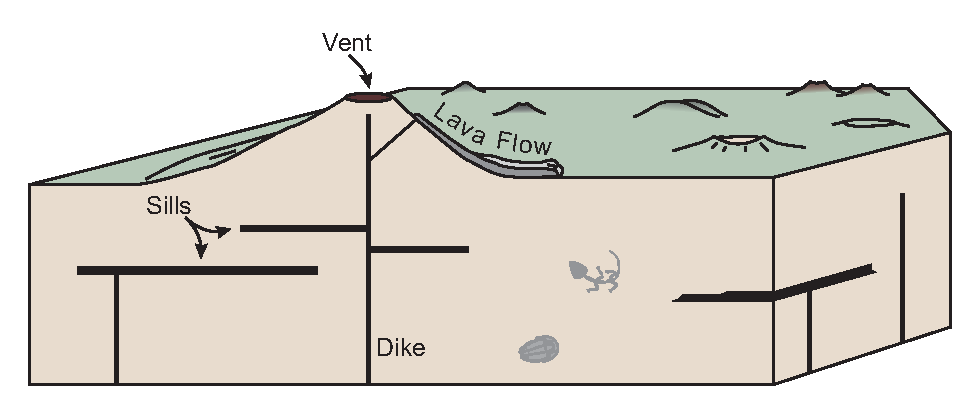
\includegraphics[width=1\textwidth]{figures/defense/distributed_cartoon.eps}
\end{columns}
\end{block}
}

\frame{\frametitle{Outline of Talk}
\begin{block}{}
\begin{columns}
	\column{.55\textwidth}
	\begin{itemize}
		\item Volcanic fields, from the inside out
			\begin{itemize}
				\item The role of sills in the formation of volcanic fields {\tiny(Richardson et al., \textit{Geology}, 2015)}
				\item The spatial organization of vents in volcanic fields {\tiny(Richardson et al., \textit{LPSC}, 2012)}
				\item Simulating lava flow emplacement {\tiny(Kubanek et al., \textit{Bull. Volc.}, 2015)}
				%\item The history of a volcanic field on Mars, Syria Planum
			\end{itemize}
		\item Evolution of volcanism at Arsia Mons
			\begin{itemize}
				\item Can its recent rate of volcanism be determined by studying a volcanic field with only satellite data?
			\end{itemize}
		\item Conclusions
	\end{itemize}
	\column{.45\textwidth}
		\centering
		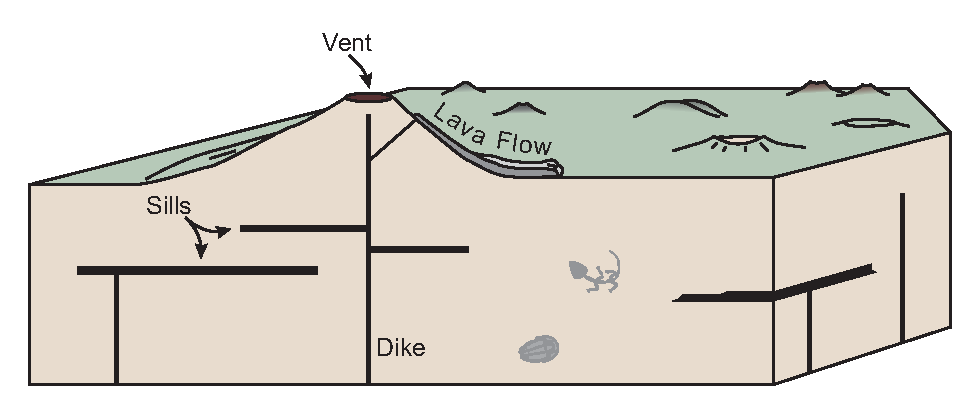
\includegraphics[width=0.8\textwidth]{figures/defense/distributed_cartoon.eps}
		
		\fbox{\includegraphics[width=0.7\textwidth,clip,trim=4.5cm 4.2cm 5cm 3cm]{figures/defense/arsia_overview.jpg}}
\end{columns}
\end{block}
}

\section{Overview}
\subsection{Sills}
	\frame{\frametitle{The Igneous Plumbing System}
	\begin{columns}
	\column{.4\textwidth}
		\begin{block}{San Rafael Volcanic Field, Utah}
		\begin{itemize}
			\item Pliocene volcanic activity
			\item Now eroded to depth of $\sim$1~km
			\item Sills and Dikes exposed
		\end{itemize}
		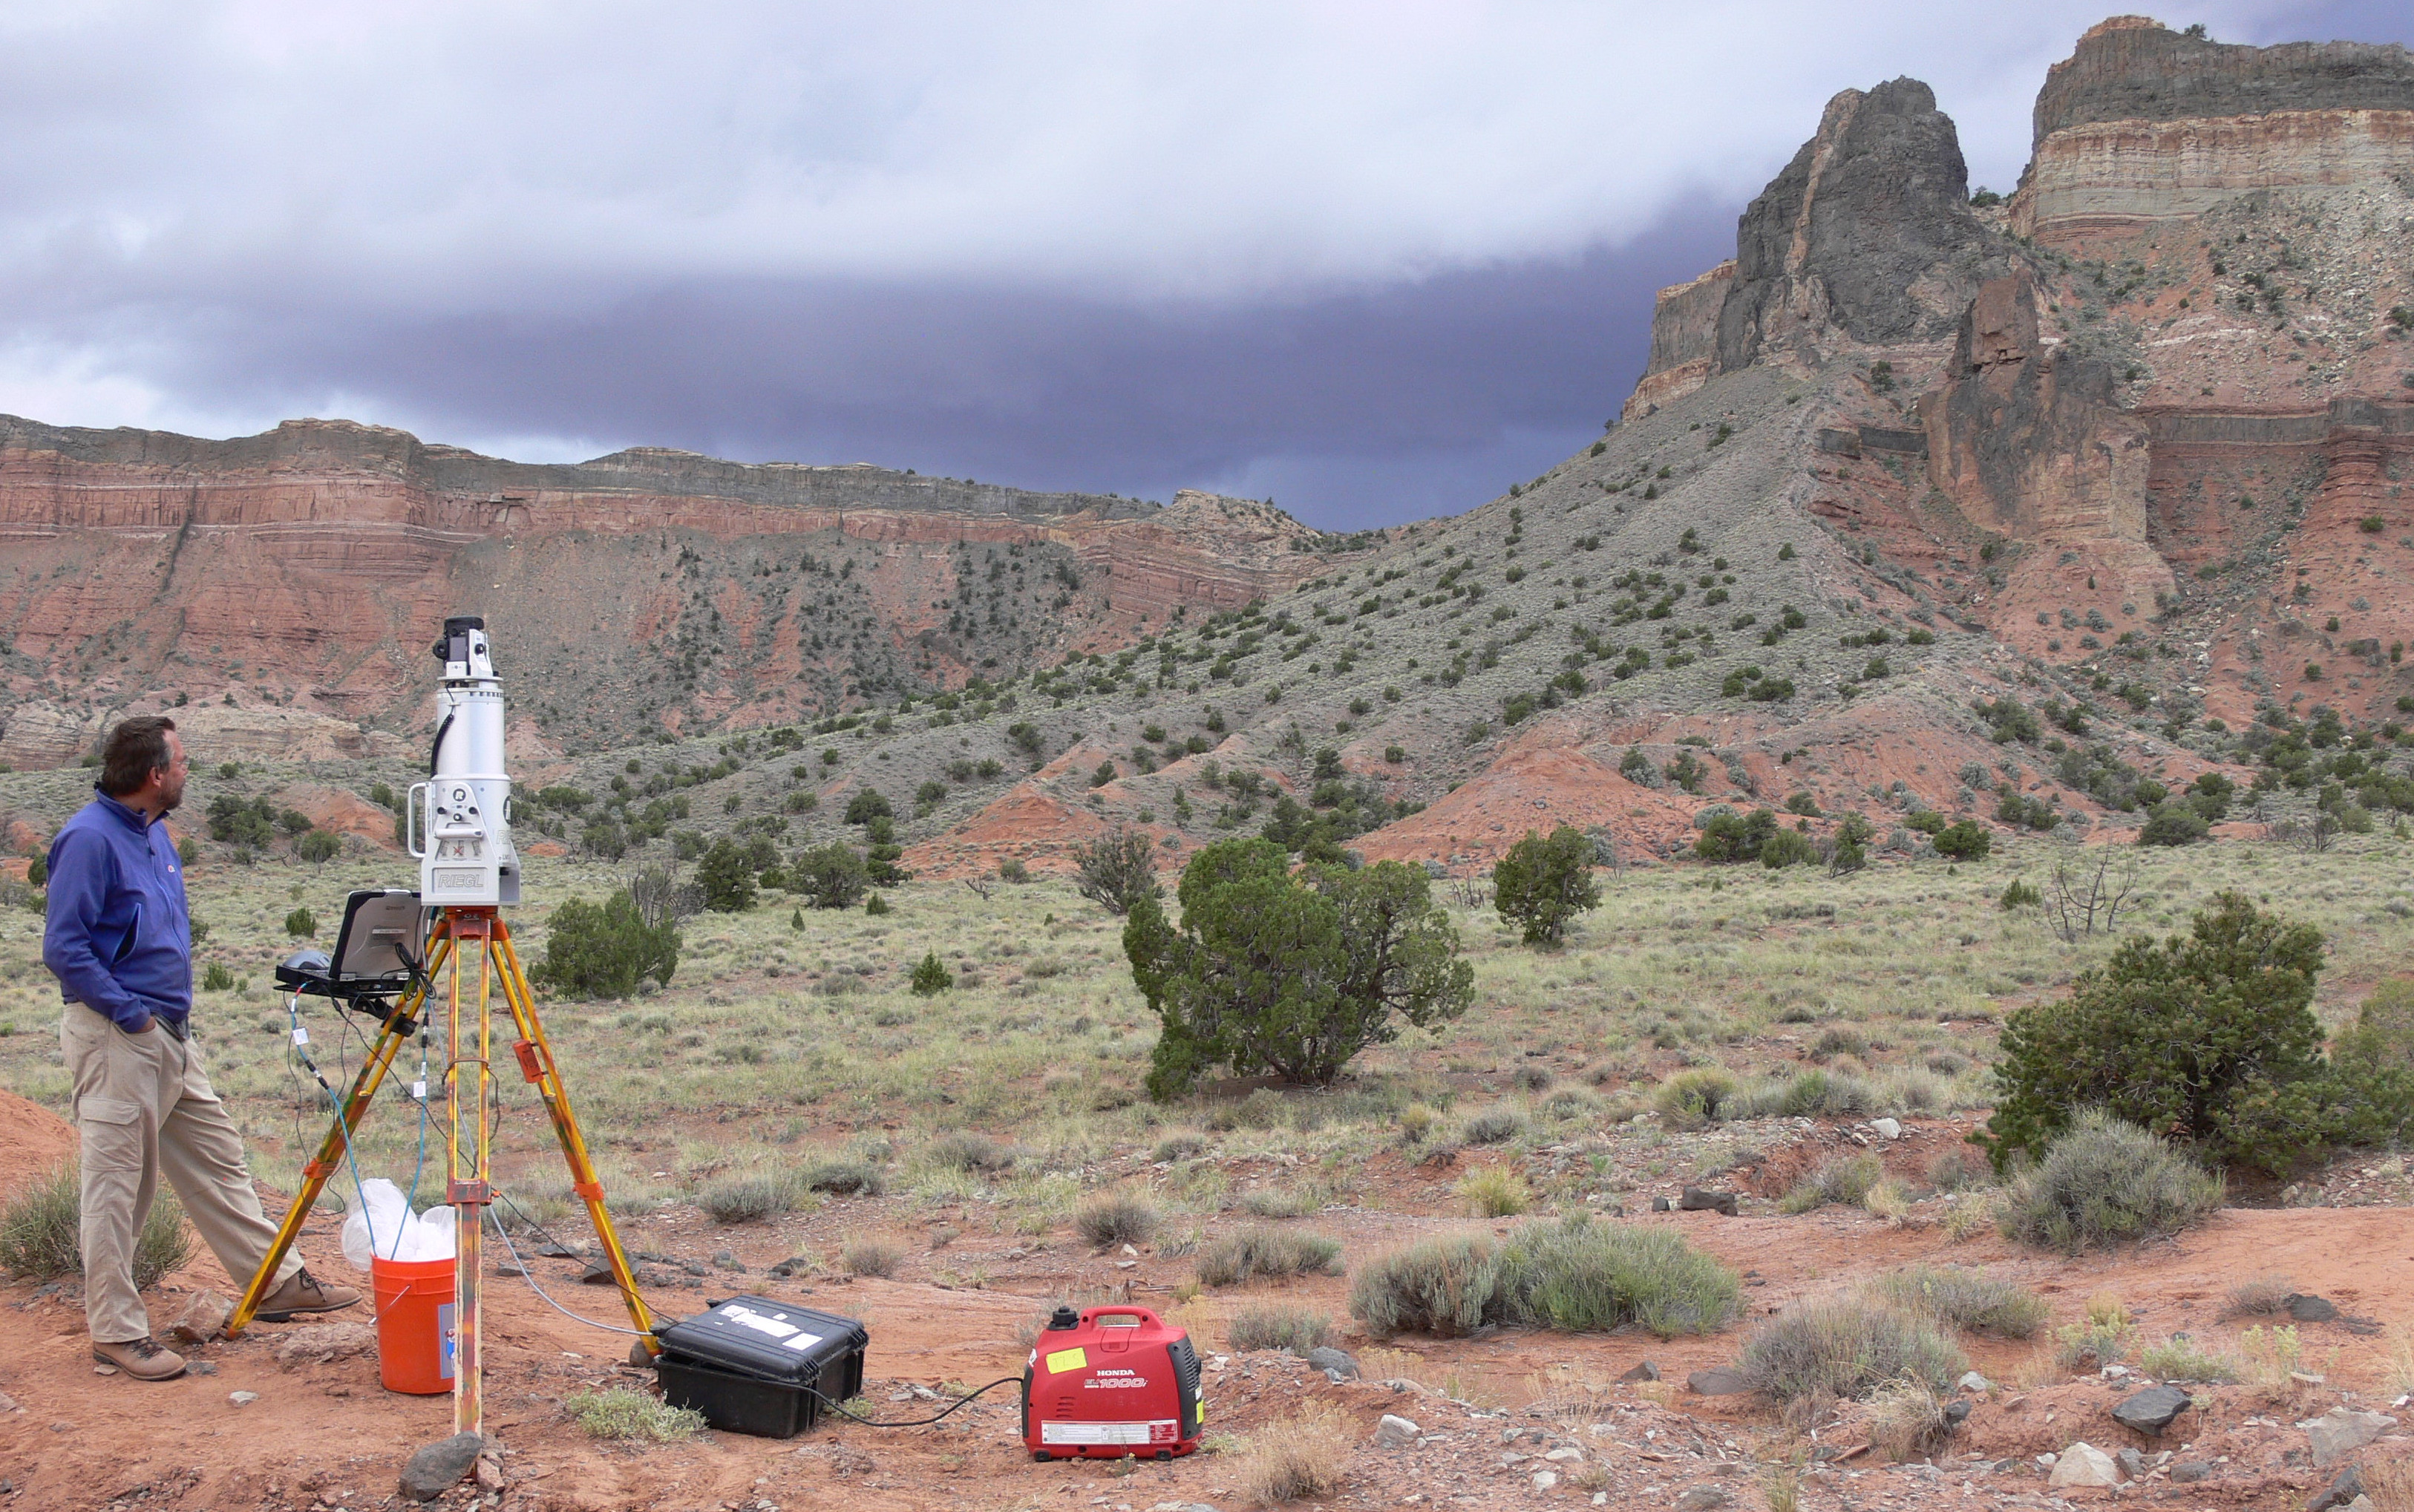
\includegraphics[width=0.9\textwidth]{figures/defense/ChuckConnor_Zlidar.jpg}\\[-0.5em]
		{\tiny Chuck Connor with a Terrestrial Lidar (L. Connor)}
		\end{block}
	\column{.6\textwidth}
		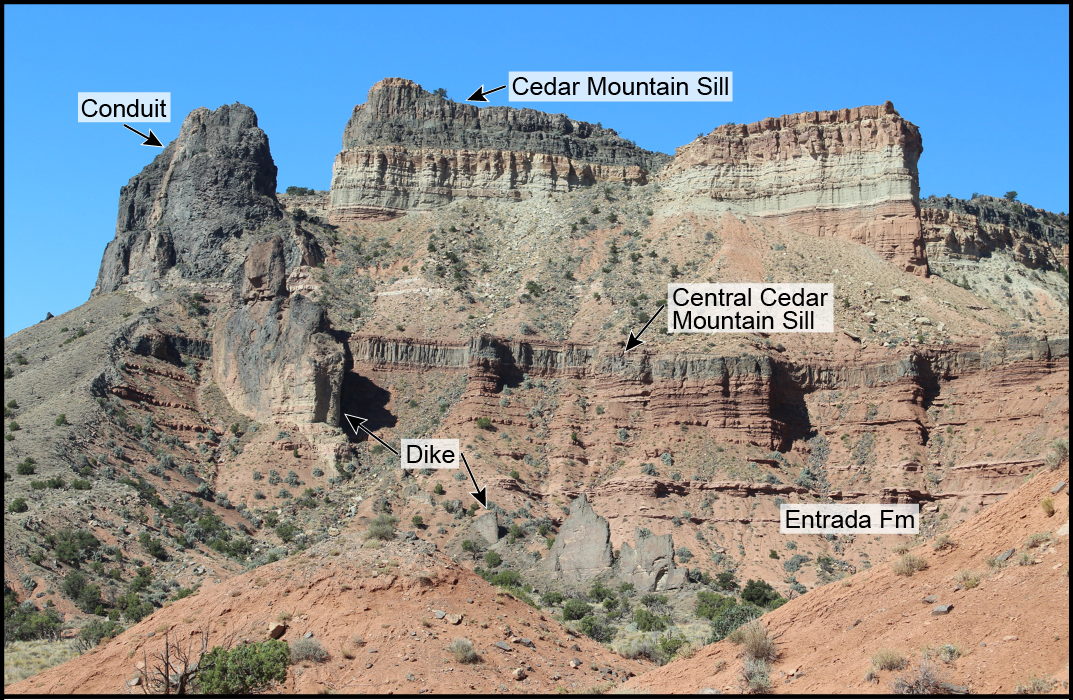
\includegraphics[width=1\textwidth]{figures/defense/CedarMtn-photo.png}\\[-0.5em]
		\mbox{\tiny \textit{Photo Credit: Judy McIlrath}}
	\end{columns}
	}

%	\frame{\frametitle{Sills in the San Rafael Swell}
%		Richardson et al., \textit{Geology}, 2015\\
%		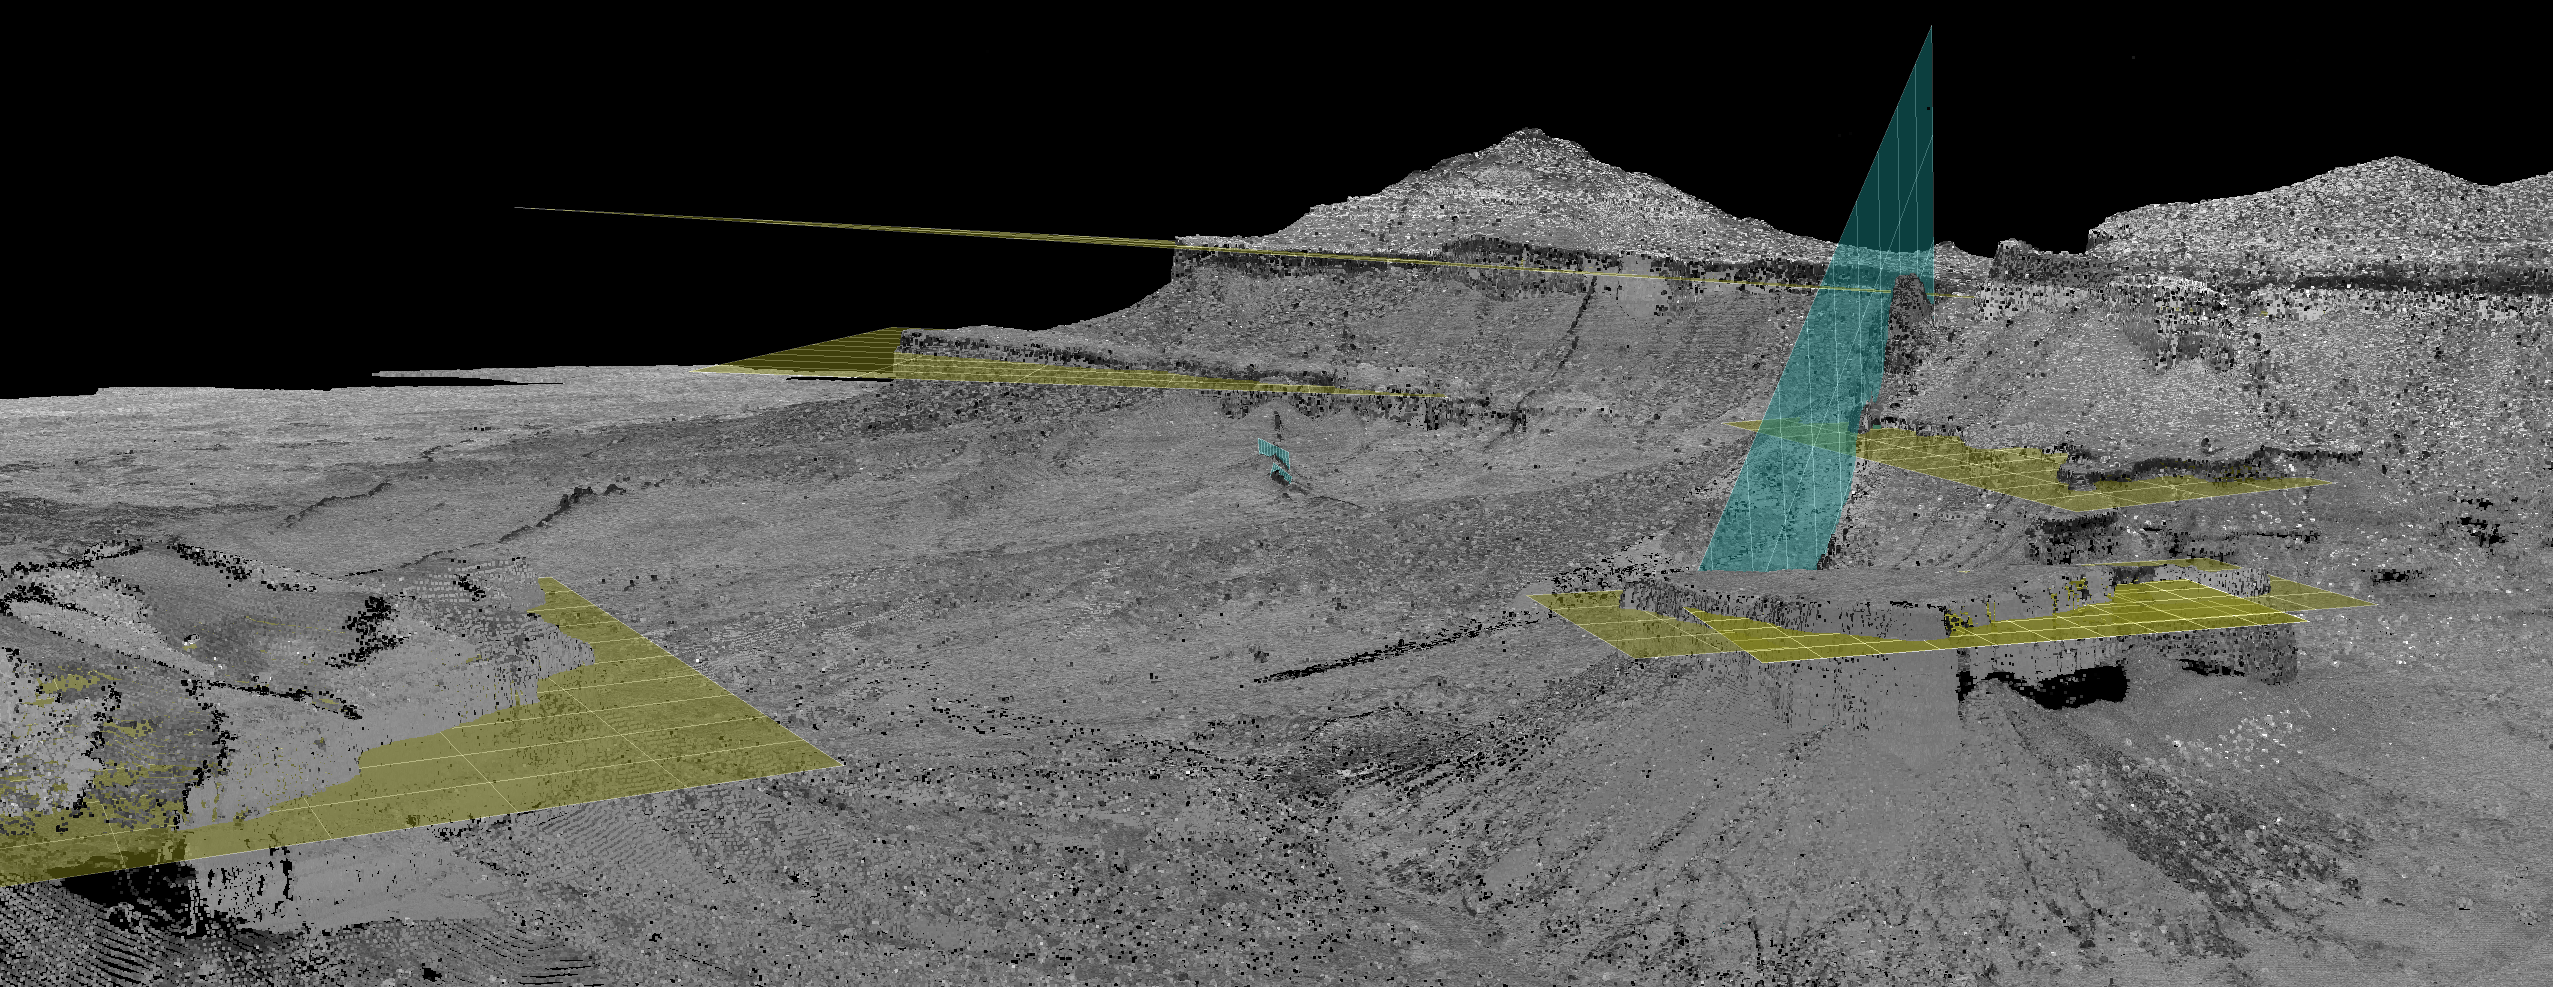
\includegraphics[width=1\textwidth]{figures/defense/lidar_screenshot.png}
%	}

	\frame{\frametitle{The Igneous Plumbing System}
	\begin{columns}
	\column{.4\textwidth}
		\begin{block}{Results of lidar survey}
		\begin{itemize}
			%\item $>$90\% of igneous rock is stored in sills
			\item Sill volume comparable to volume thought to have erupted at surface
			\item Sills had ability to modulate eruption style by interacting with volcanic conduits
			\item Conduits deliver magma from depth to distributed volcanoes
		\end{itemize}
		\end{block}
	\column{.6\textwidth}
		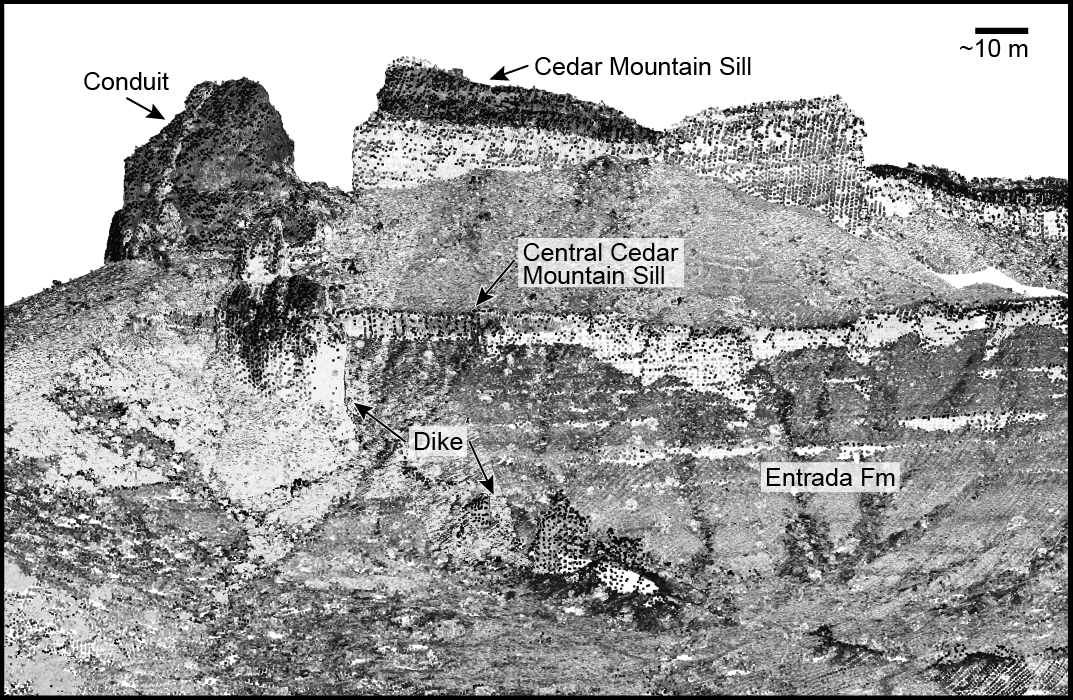
\includegraphics[width=1\textwidth]{figures/defense/CedarMtn-pcloud.png}\\[-0.5em]
		\mbox{\tiny \textit{Richardson et al., Geology, 2015}}
	\end{columns}
	}

\iffalse
	\frame{\frametitle{Sills in the San Rafael Swell}
	\begin{columns}
	\column{.6\textwidth}
		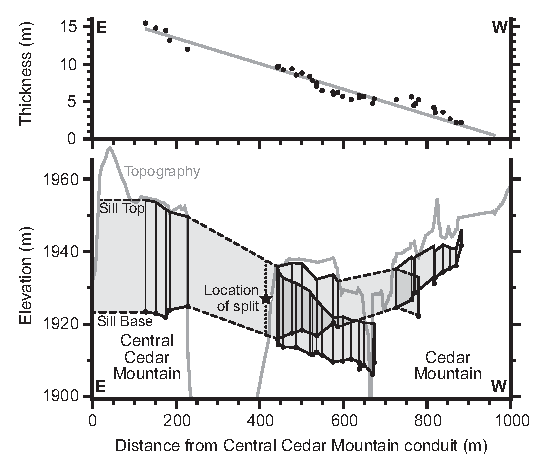
\includegraphics[width=0.5\textwidth]{figures/chapter-sills/Fig4-chart.eps}
		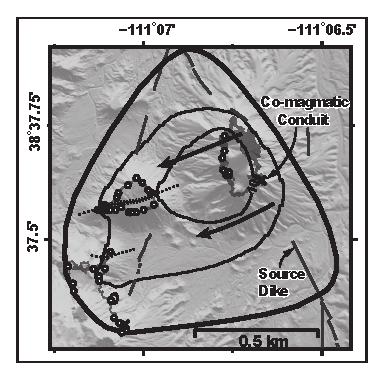
\includegraphics[width=0.5\textwidth]{figures/defense/ccm_model.eps}
	\column{.4\textwidth}
		\begin{block}{}
		\begin{itemize}
			\item Lidar
			\item Sills
			\item Total volume, geometry
			\item Modulation of eruption style
		\end{itemize}
		\end{block}
	\end{columns}
	}
\fi

%%%%%%%%%%%%%%%%%%%%%%%%%%%%%
%Vent Density
\subsection{Vent Intensity}
	\frame{\frametitle{Volcano organization in fields}
		\begin{center}
			The spatial organization of volcanoes is modeled as a density function\\
			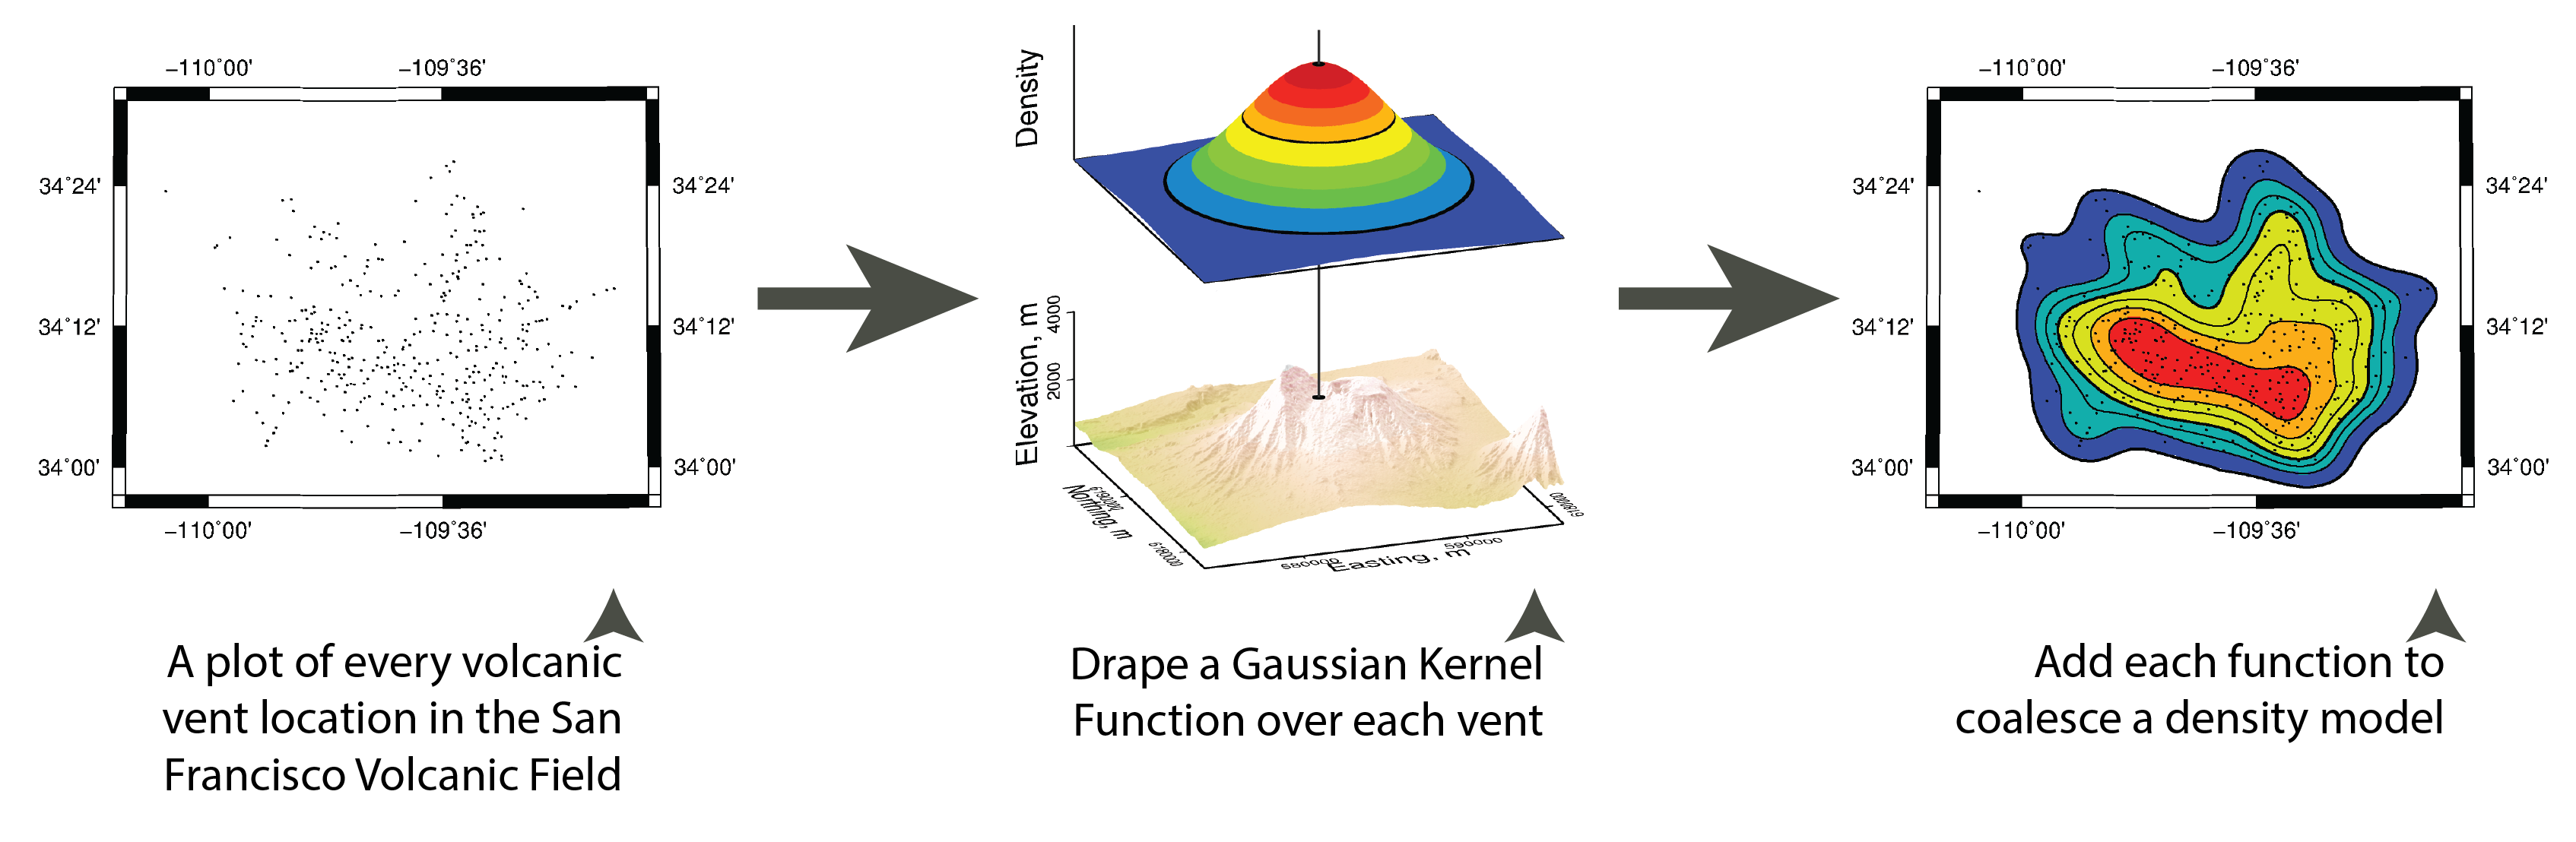
\includegraphics[width=0.8\textwidth]{figures/defense/kde_build_300dpi.png}
		\end{center}\\[-0.5em]
		\begin{block}{}
		\begin{itemize}
			\item Area of volcanic field defined as 95$^{\text th}$ percentile of density function\\[-0.5em]
			\begin{equation*}
			\text{Average vent intensity} = \frac{\text{\# volcanic vents}}{\text{field area}} \end{equation*}
			\item This model is applied to fields on Earth, Mars, and Venus
		\end{itemize}
		\end{block}
		
	}

	\frame{\frametitle{Vent Spatial Intensity across the Solar System}
		\begin{columns}
		\column{.7\textwidth}
			\begin{block}{Average Vent Intensity, Colored by Planet}
			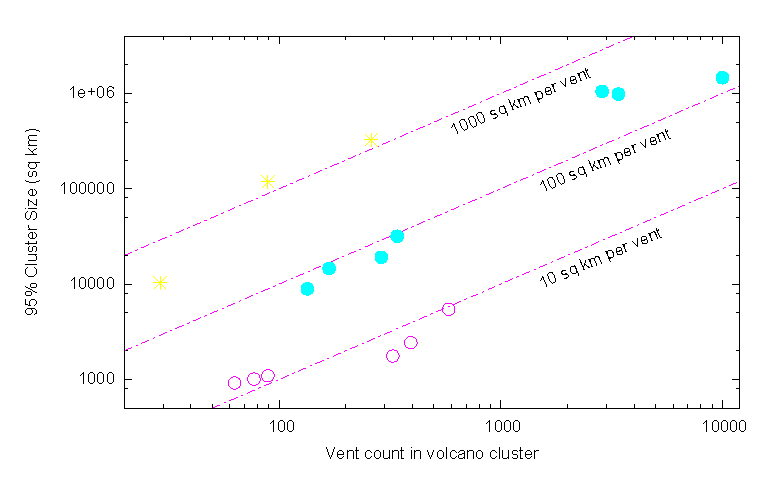
\includegraphics[width=0.9\textwidth]{figures/defense/cluster_dens.eps}
			\end{block}
			%% GNUPLOT: LaTeX picture
\setlength{\unitlength}{0.240900pt}
\ifx\plotpoint\undefined\newsavebox{\plotpoint}\fi
\sbox{\plotpoint}{\rule[-0.200pt]{0.400pt}{0.400pt}}%
\begin{picture}(1500,900)(0,0)
\sbox{\plotpoint}{\rule[-0.200pt]{0.400pt}{0.400pt}}%
\put(231.0,131.0){\rule[-0.200pt]{2.409pt}{0.400pt}}
\put(1429.0,131.0){\rule[-0.200pt]{2.409pt}{0.400pt}}
\put(231.0,169.0){\rule[-0.200pt]{2.409pt}{0.400pt}}
\put(1429.0,169.0){\rule[-0.200pt]{2.409pt}{0.400pt}}
\put(231.0,187.0){\rule[-0.200pt]{4.818pt}{0.400pt}}
\put(211,187){\makebox(0,0)[r]{ 1000}}
\put(1419.0,187.0){\rule[-0.200pt]{4.818pt}{0.400pt}}
\put(231.0,243.0){\rule[-0.200pt]{2.409pt}{0.400pt}}
\put(1429.0,243.0){\rule[-0.200pt]{2.409pt}{0.400pt}}
\put(231.0,318.0){\rule[-0.200pt]{2.409pt}{0.400pt}}
\put(1429.0,318.0){\rule[-0.200pt]{2.409pt}{0.400pt}}
\put(231.0,356.0){\rule[-0.200pt]{2.409pt}{0.400pt}}
\put(1429.0,356.0){\rule[-0.200pt]{2.409pt}{0.400pt}}
\put(231.0,374.0){\rule[-0.200pt]{4.818pt}{0.400pt}}
\put(211,374){\makebox(0,0)[r]{ 10000}}
\put(1419.0,374.0){\rule[-0.200pt]{4.818pt}{0.400pt}}
\put(231.0,430.0){\rule[-0.200pt]{2.409pt}{0.400pt}}
\put(1429.0,430.0){\rule[-0.200pt]{2.409pt}{0.400pt}}
\put(231.0,504.0){\rule[-0.200pt]{2.409pt}{0.400pt}}
\put(1429.0,504.0){\rule[-0.200pt]{2.409pt}{0.400pt}}
\put(231.0,542.0){\rule[-0.200pt]{2.409pt}{0.400pt}}
\put(1429.0,542.0){\rule[-0.200pt]{2.409pt}{0.400pt}}
\put(231.0,560.0){\rule[-0.200pt]{4.818pt}{0.400pt}}
\put(211,560){\makebox(0,0)[r]{ 100000}}
\put(1419.0,560.0){\rule[-0.200pt]{4.818pt}{0.400pt}}
\put(231.0,616.0){\rule[-0.200pt]{2.409pt}{0.400pt}}
\put(1429.0,616.0){\rule[-0.200pt]{2.409pt}{0.400pt}}
\put(231.0,691.0){\rule[-0.200pt]{2.409pt}{0.400pt}}
\put(1429.0,691.0){\rule[-0.200pt]{2.409pt}{0.400pt}}
\put(231.0,729.0){\rule[-0.200pt]{2.409pt}{0.400pt}}
\put(1429.0,729.0){\rule[-0.200pt]{2.409pt}{0.400pt}}
\put(231.0,747.0){\rule[-0.200pt]{4.818pt}{0.400pt}}
\put(211,747){\makebox(0,0)[r]{ 1e+06}}
\put(1419.0,747.0){\rule[-0.200pt]{4.818pt}{0.400pt}}
\put(231.0,803.0){\rule[-0.200pt]{2.409pt}{0.400pt}}
\put(1429.0,803.0){\rule[-0.200pt]{2.409pt}{0.400pt}}
\put(231.0,131.0){\rule[-0.200pt]{0.400pt}{2.409pt}}
\put(231.0,849.0){\rule[-0.200pt]{0.400pt}{2.409pt}}
\put(308.0,131.0){\rule[-0.200pt]{0.400pt}{2.409pt}}
\put(308.0,849.0){\rule[-0.200pt]{0.400pt}{2.409pt}}
\put(362.0,131.0){\rule[-0.200pt]{0.400pt}{2.409pt}}
\put(362.0,849.0){\rule[-0.200pt]{0.400pt}{2.409pt}}
\put(404.0,131.0){\rule[-0.200pt]{0.400pt}{2.409pt}}
\put(404.0,849.0){\rule[-0.200pt]{0.400pt}{2.409pt}}
\put(438.0,131.0){\rule[-0.200pt]{0.400pt}{2.409pt}}
\put(438.0,849.0){\rule[-0.200pt]{0.400pt}{2.409pt}}
\put(468.0,131.0){\rule[-0.200pt]{0.400pt}{2.409pt}}
\put(468.0,849.0){\rule[-0.200pt]{0.400pt}{2.409pt}}
\put(493.0,131.0){\rule[-0.200pt]{0.400pt}{2.409pt}}
\put(493.0,849.0){\rule[-0.200pt]{0.400pt}{2.409pt}}
\put(515.0,131.0){\rule[-0.200pt]{0.400pt}{2.409pt}}
\put(515.0,849.0){\rule[-0.200pt]{0.400pt}{2.409pt}}
\put(535.0,131.0){\rule[-0.200pt]{0.400pt}{4.818pt}}
\put(535,90){\makebox(0,0){ 100}}
\put(535.0,839.0){\rule[-0.200pt]{0.400pt}{4.818pt}}
\put(666.0,131.0){\rule[-0.200pt]{0.400pt}{2.409pt}}
\put(666.0,849.0){\rule[-0.200pt]{0.400pt}{2.409pt}}
\put(742.0,131.0){\rule[-0.200pt]{0.400pt}{2.409pt}}
\put(742.0,849.0){\rule[-0.200pt]{0.400pt}{2.409pt}}
\put(797.0,131.0){\rule[-0.200pt]{0.400pt}{2.409pt}}
\put(797.0,849.0){\rule[-0.200pt]{0.400pt}{2.409pt}}
\put(839.0,131.0){\rule[-0.200pt]{0.400pt}{2.409pt}}
\put(839.0,849.0){\rule[-0.200pt]{0.400pt}{2.409pt}}
\put(873.0,131.0){\rule[-0.200pt]{0.400pt}{2.409pt}}
\put(873.0,849.0){\rule[-0.200pt]{0.400pt}{2.409pt}}
\put(902.0,131.0){\rule[-0.200pt]{0.400pt}{2.409pt}}
\put(902.0,849.0){\rule[-0.200pt]{0.400pt}{2.409pt}}
\put(928.0,131.0){\rule[-0.200pt]{0.400pt}{2.409pt}}
\put(928.0,849.0){\rule[-0.200pt]{0.400pt}{2.409pt}}
\put(950.0,131.0){\rule[-0.200pt]{0.400pt}{2.409pt}}
\put(950.0,849.0){\rule[-0.200pt]{0.400pt}{2.409pt}}
\put(970.0,131.0){\rule[-0.200pt]{0.400pt}{4.818pt}}
\put(970,90){\makebox(0,0){ 1000}}
\put(970.0,839.0){\rule[-0.200pt]{0.400pt}{4.818pt}}
\put(1101.0,131.0){\rule[-0.200pt]{0.400pt}{2.409pt}}
\put(1101.0,849.0){\rule[-0.200pt]{0.400pt}{2.409pt}}
\put(1177.0,131.0){\rule[-0.200pt]{0.400pt}{2.409pt}}
\put(1177.0,849.0){\rule[-0.200pt]{0.400pt}{2.409pt}}
\put(1232.0,131.0){\rule[-0.200pt]{0.400pt}{2.409pt}}
\put(1232.0,849.0){\rule[-0.200pt]{0.400pt}{2.409pt}}
\put(1274.0,131.0){\rule[-0.200pt]{0.400pt}{2.409pt}}
\put(1274.0,849.0){\rule[-0.200pt]{0.400pt}{2.409pt}}
\put(1308.0,131.0){\rule[-0.200pt]{0.400pt}{2.409pt}}
\put(1308.0,849.0){\rule[-0.200pt]{0.400pt}{2.409pt}}
\put(1337.0,131.0){\rule[-0.200pt]{0.400pt}{2.409pt}}
\put(1337.0,849.0){\rule[-0.200pt]{0.400pt}{2.409pt}}
\put(1362.0,131.0){\rule[-0.200pt]{0.400pt}{2.409pt}}
\put(1362.0,849.0){\rule[-0.200pt]{0.400pt}{2.409pt}}
\put(1385.0,131.0){\rule[-0.200pt]{0.400pt}{2.409pt}}
\put(1385.0,849.0){\rule[-0.200pt]{0.400pt}{2.409pt}}
\put(1405.0,131.0){\rule[-0.200pt]{0.400pt}{4.818pt}}
\put(1405,90){\makebox(0,0){ 10000}}
\put(1405.0,839.0){\rule[-0.200pt]{0.400pt}{4.818pt}}
\put(231.0,131.0){\rule[-0.200pt]{0.400pt}{175.375pt}}
\put(231.0,131.0){\rule[-0.200pt]{291.007pt}{0.400pt}}
\put(1439.0,131.0){\rule[-0.200pt]{0.400pt}{175.375pt}}
\put(231.0,859.0){\rule[-0.200pt]{291.007pt}{0.400pt}}
\put(30,495){\rotatebox{-270}{\makebox(0,0){2-$sigma$ Cluster Size (km$^2$)}}
}\put(835,29){\makebox(0,0){Vent count in volcano cluster}}
\put(1046,374){\rotatebox{23}{\makebox(0,0)[l]{10 km$^2$ per vent}}
}\put(1046,560){\rotatebox{23}{\makebox(0,0)[l]{100 km$^2$ per vent}}
}\put(873,672){\rotatebox{23}{\makebox(0,0)[l]{1000 km$^2$ per vent}}
}\sbox{\plotpoint}{\rule[-0.500pt]{1.000pt}{1.000pt}}%
\multiput(404,131)(19.085,8.158){7}{\usebox{\plotpoint}}
\multiput(535,187)(19.068,8.197){23}{\usebox{\plotpoint}}
\multiput(970,374)(19.084,8.160){23}{\usebox{\plotpoint}}
\multiput(1405,560)(18.990,8.378){2}{\usebox{\plotpoint}}
\put(1439,575){\usebox{\plotpoint}}
\multiput(231,243)(19.061,8.214){16}{\usebox{\plotpoint}}
\multiput(535,374)(19.084,8.160){23}{\usebox{\plotpoint}}
\multiput(970,560)(19.068,8.197){23}{\usebox{\plotpoint}}
\multiput(1405,747)(19.192,7.903){2}{\usebox{\plotpoint}}
\put(1439,761){\usebox{\plotpoint}}
\multiput(231,430)(19.084,8.161){16}{\usebox{\plotpoint}}
\multiput(535,560)(19.068,8.197){23}{\usebox{\plotpoint}}
\multiput(970,747)(19.085,8.158){14}{\usebox{\plotpoint}}
\put(1232,859){\usebox{\plotpoint}}
\sbox{\plotpoint}{\rule[-0.200pt]{0.400pt}{0.400pt}}%
\put(571,819){\makebox(0,0)[r]{  Earth Clusters}}
\sbox{\plotpoint}{\rule[-0.500pt]{1.000pt}{1.000pt}}%
\put(486,188){\makebox(0,0){$\circ$}}
\put(868,324){\makebox(0,0){$\circ$}}
\put(448,180){\makebox(0,0){$\circ$}}
\put(793,259){\makebox(0,0){$\circ$}}
\put(513,194){\makebox(0,0){$\circ$}}
\put(758,233){\makebox(0,0){$\circ$}}
\put(641,819){\makebox(0,0){$\circ$}}
\sbox{\plotpoint}{\rule[-0.600pt]{1.200pt}{1.200pt}}%
\sbox{\plotpoint}{\rule[-0.200pt]{0.400pt}{0.400pt}}%
\put(571,778){\makebox(0,0)[r]{  Venus Clusters}}
\sbox{\plotpoint}{\rule[-0.600pt]{1.200pt}{1.200pt}}%
\put(767,467){\makebox(0,0){$\bullet$}}
\put(590,364){\makebox(0,0){$\bullet$}}
\put(633,404){\makebox(0,0){$\bullet$}}
\put(735,426){\makebox(0,0){$\bullet$}}
\put(1169,751){\makebox(0,0){$\bullet$}}
\put(1405,777){\makebox(0,0){$\bullet$}}
\put(1201,746){\makebox(0,0){$\bullet$}}
\put(641,778){\makebox(0,0){$\bullet$}}
\sbox{\plotpoint}{\rule[-0.500pt]{1.000pt}{1.000pt}}%
\sbox{\plotpoint}{\rule[-0.200pt]{0.400pt}{0.400pt}}%
\put(571,737){\makebox(0,0)[r]{  Mars Clusters}}
\sbox{\plotpoint}{\rule[-0.500pt]{1.000pt}{1.000pt}}%
\put(301,376){\makebox(0,0){$\ast$}}
\put(513,574){\makebox(0,0){$\ast$}}
\put(715,656){\makebox(0,0){$\ast$}}
\put(641,737){\makebox(0,0){$\ast$}}
\sbox{\plotpoint}{\rule[-0.200pt]{0.400pt}{0.400pt}}%
\put(231.0,131.0){\rule[-0.200pt]{0.400pt}{175.375pt}}
\put(231.0,131.0){\rule[-0.200pt]{291.007pt}{0.400pt}}
\put(1439.0,131.0){\rule[-0.200pt]{0.400pt}{175.375pt}}
\put(231.0,859.0){\rule[-0.200pt]{291.007pt}{0.400pt}}
\end{picture}

		\column{.2\textwidth}
			\begin{center}
			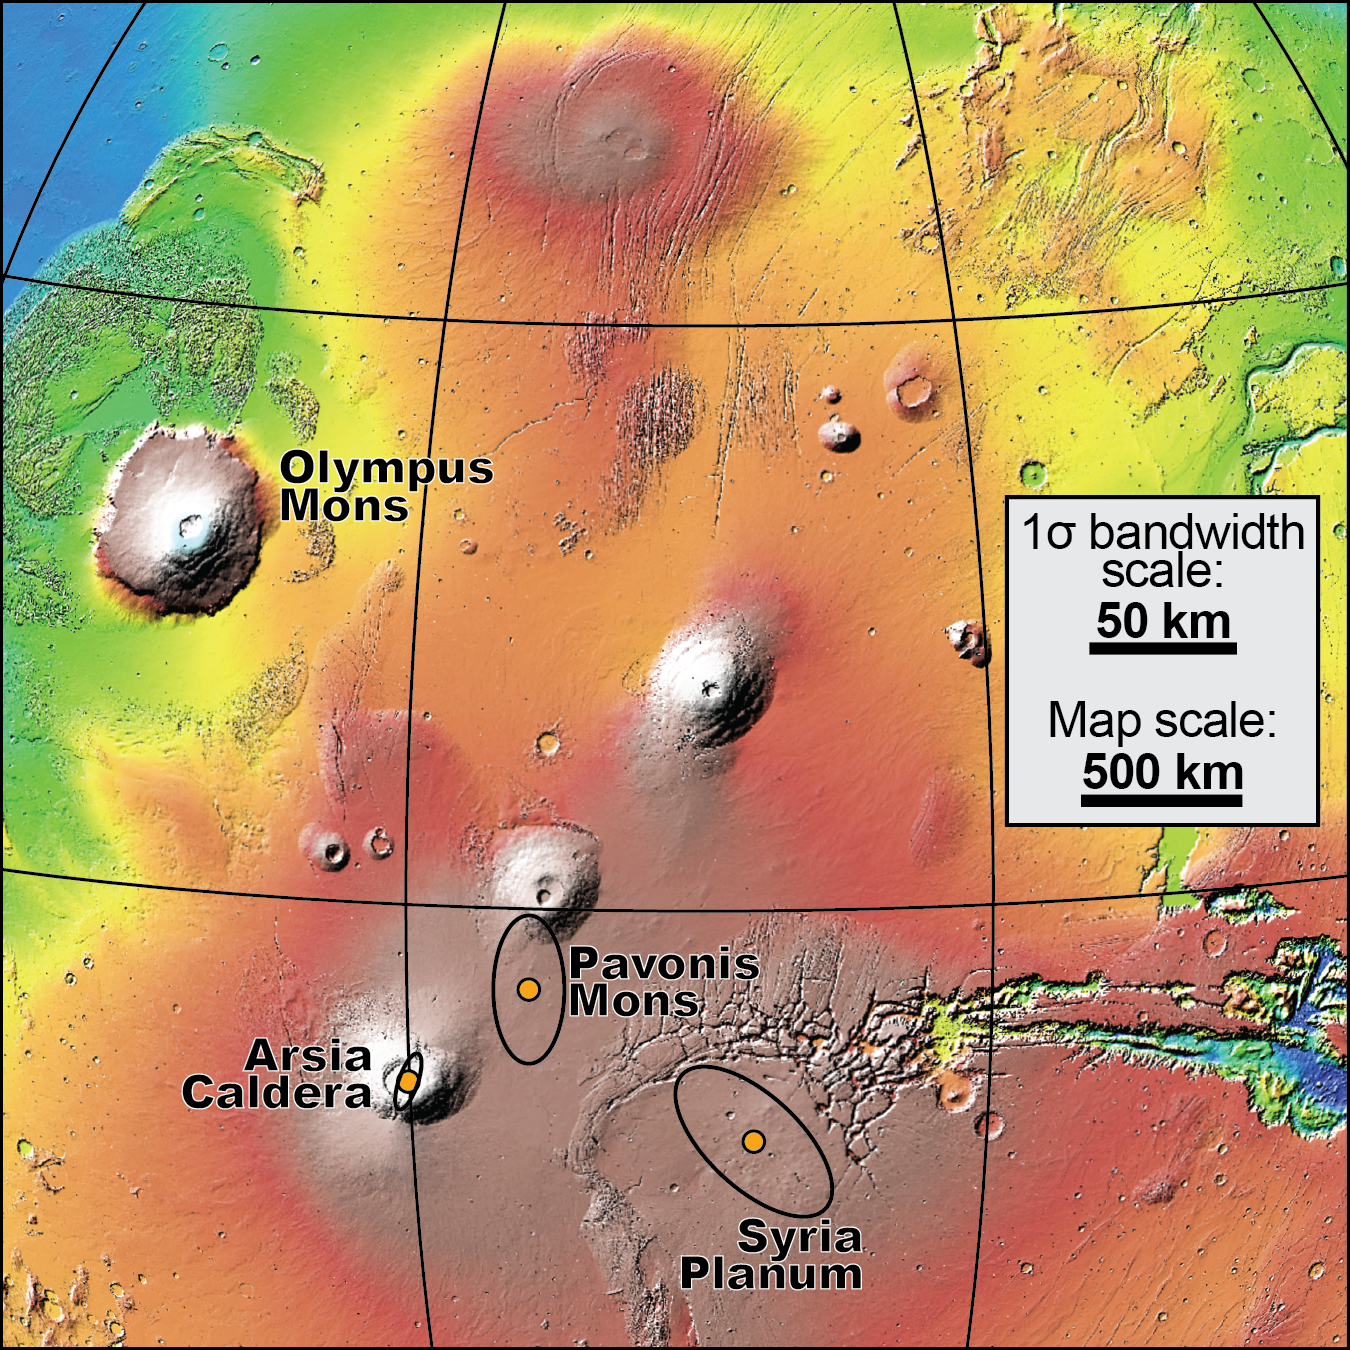
\includegraphics[width=0.8\textwidth]{figures/defense/mars_locator_300dpi}
			
			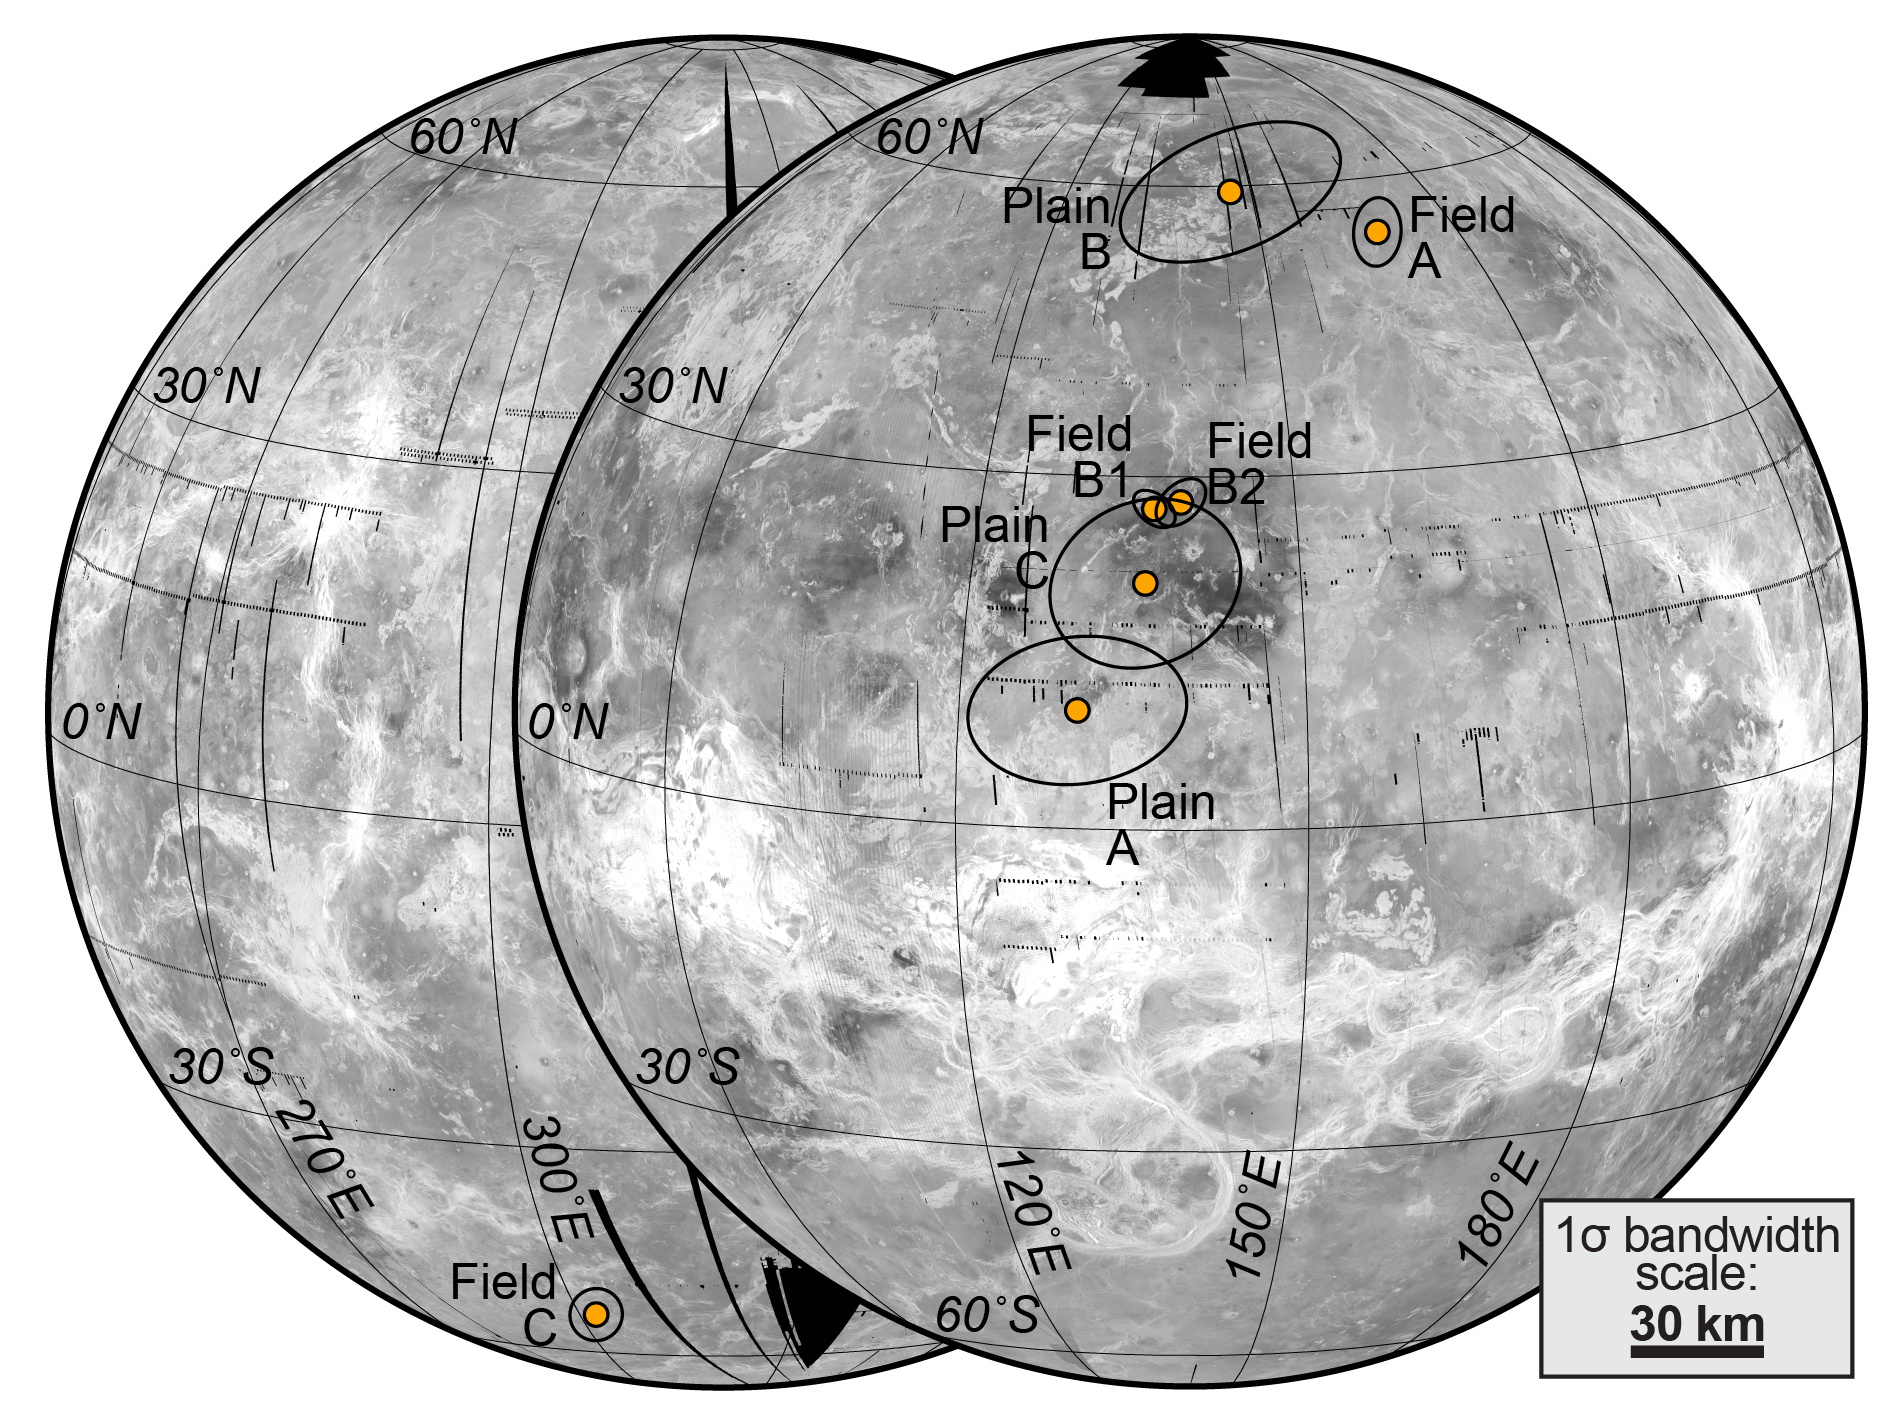
\includegraphics[width=0.9\textwidth]{figures/defense/venus_globe_300dpi}
			
			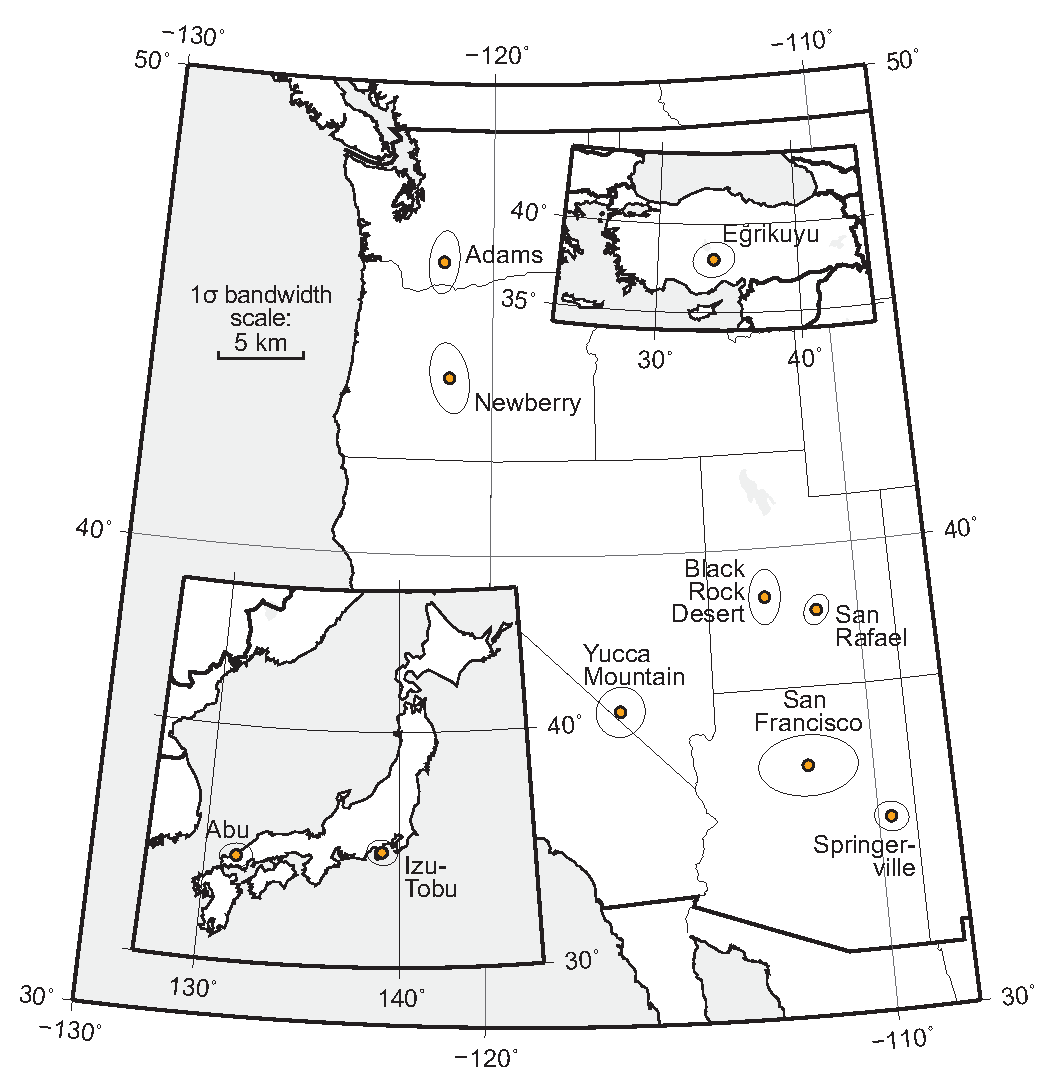
\includegraphics[width=0.9\textwidth]{figures/chapter-spatial_density/locators/earth_locator.eps}
			\end{center}
		\end{columns}
	}
	
%%%%%%%%%%%%%%%%%%%%%%%%%%%%%
%LAVA FLOWS
\subsection{Lava Flows}
	\frame{\frametitle{The 2012-3 Tolbachik Lava Flow}
		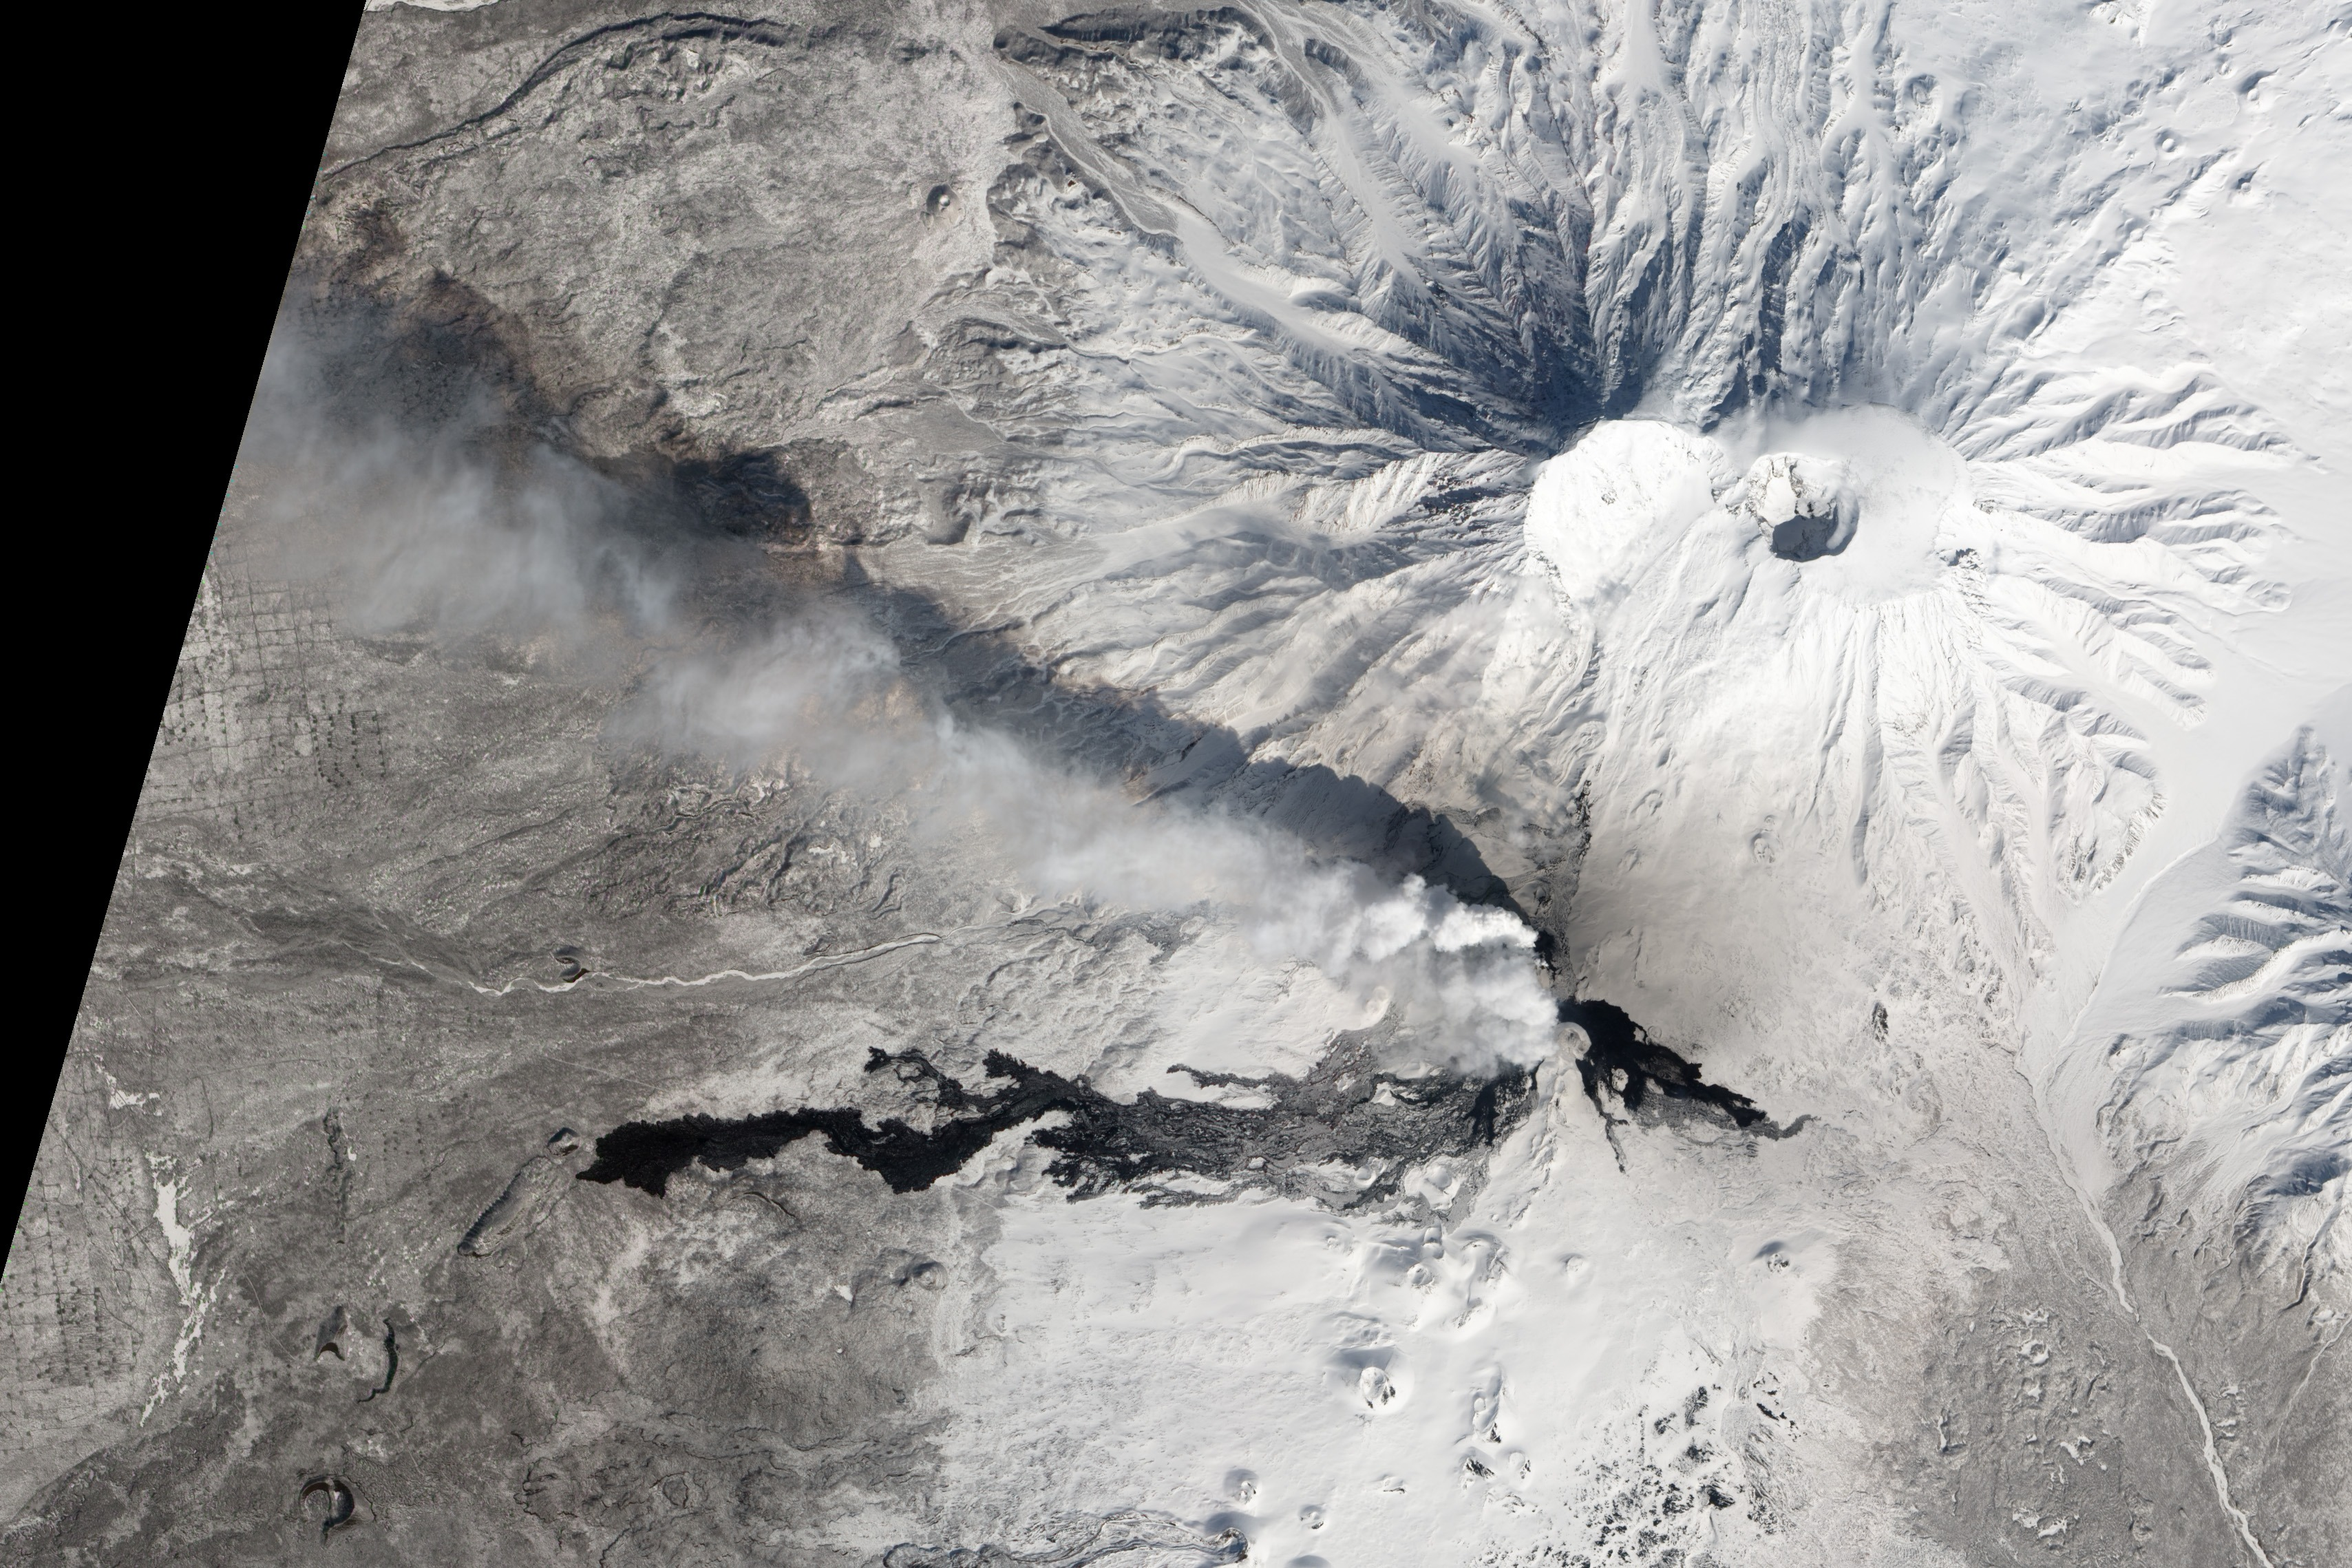
\includegraphics[width=1\textwidth,clip,trim=5cm 10cm 5cm 16cm]{figures/defense/tolbachik_eo1.png}\\[-0.5em]
		\mbox{\tiny \textit{NASA Earth Observing-1 Mission, 1 February 2013}}
	}
	
	\frame{\frametitle{Lava Flows/Simulators}
	%\begin{columns}
	%\column{.23\textwidth}
		%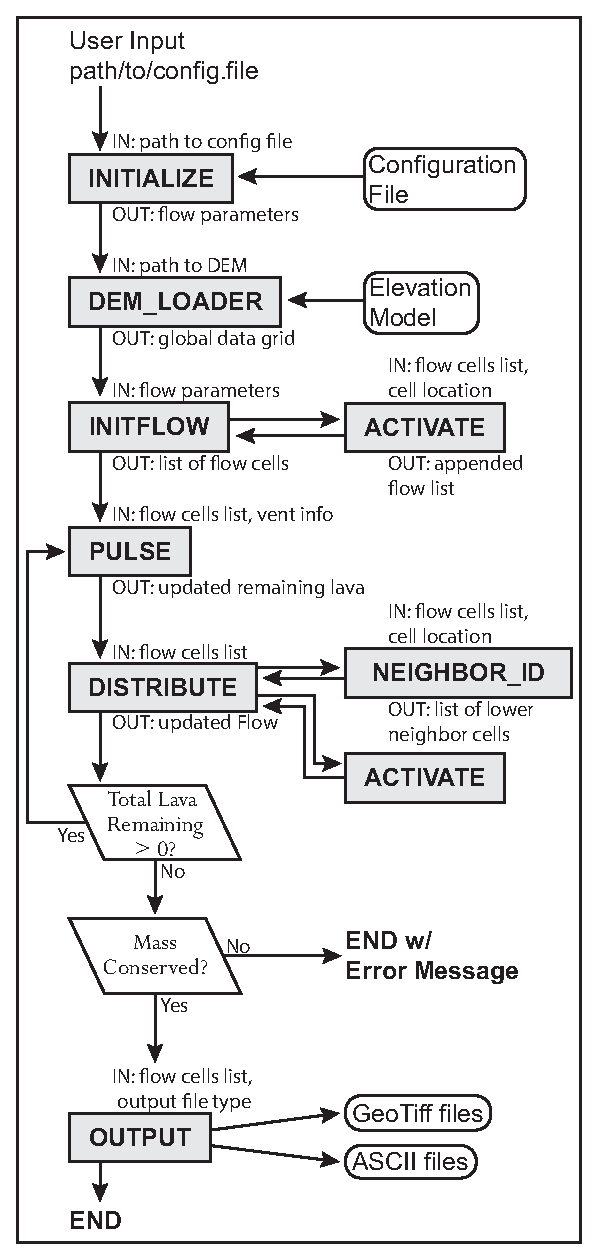
\includegraphics[width=1\textwidth]{figures/chapter-molasses/Flow_Chart.eps}
	%\column{.77\textwidth}
		\begin{block}{MOLASSES --- Modular Lava Simulation Software}
		\begin{columns}
		\column{.5\textwidth}
			\begin{itemize}
				\item MOLASSES developed after \mbox{Connor et al., \textit{JAV}, 2012}
				\item Spreads lava over a grid according to universal rules
			\end{itemize}
			\begin{block}{Optional Spreading Rules}
				\centering
				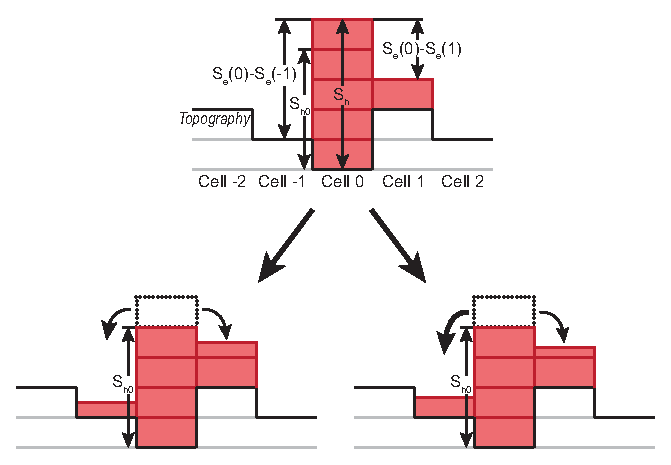
\includegraphics[width=0.5\textwidth]{figures/chapter-molasses/slope-proportional-example.eps}
				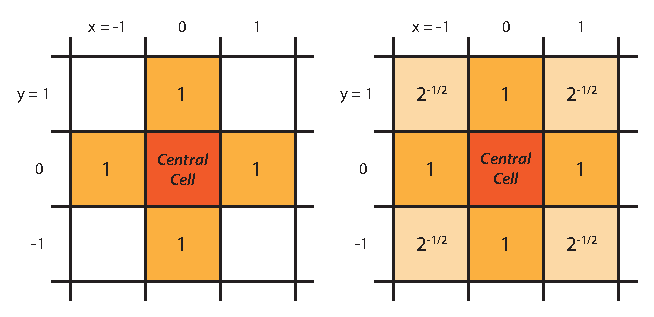
\includegraphics[width=0.5\textwidth,clip,trim=0cm 0cm 0cm 0cm]{figures/chapter-molasses/neighborhoods.eps}
			\end{block}
		\column{.5\textwidth}
		Using TanDEM-X satellite data, flow simulations match the 2012-3 Tolbachik flow between 70-85\%.\\[-2em]
		\begin{center}
		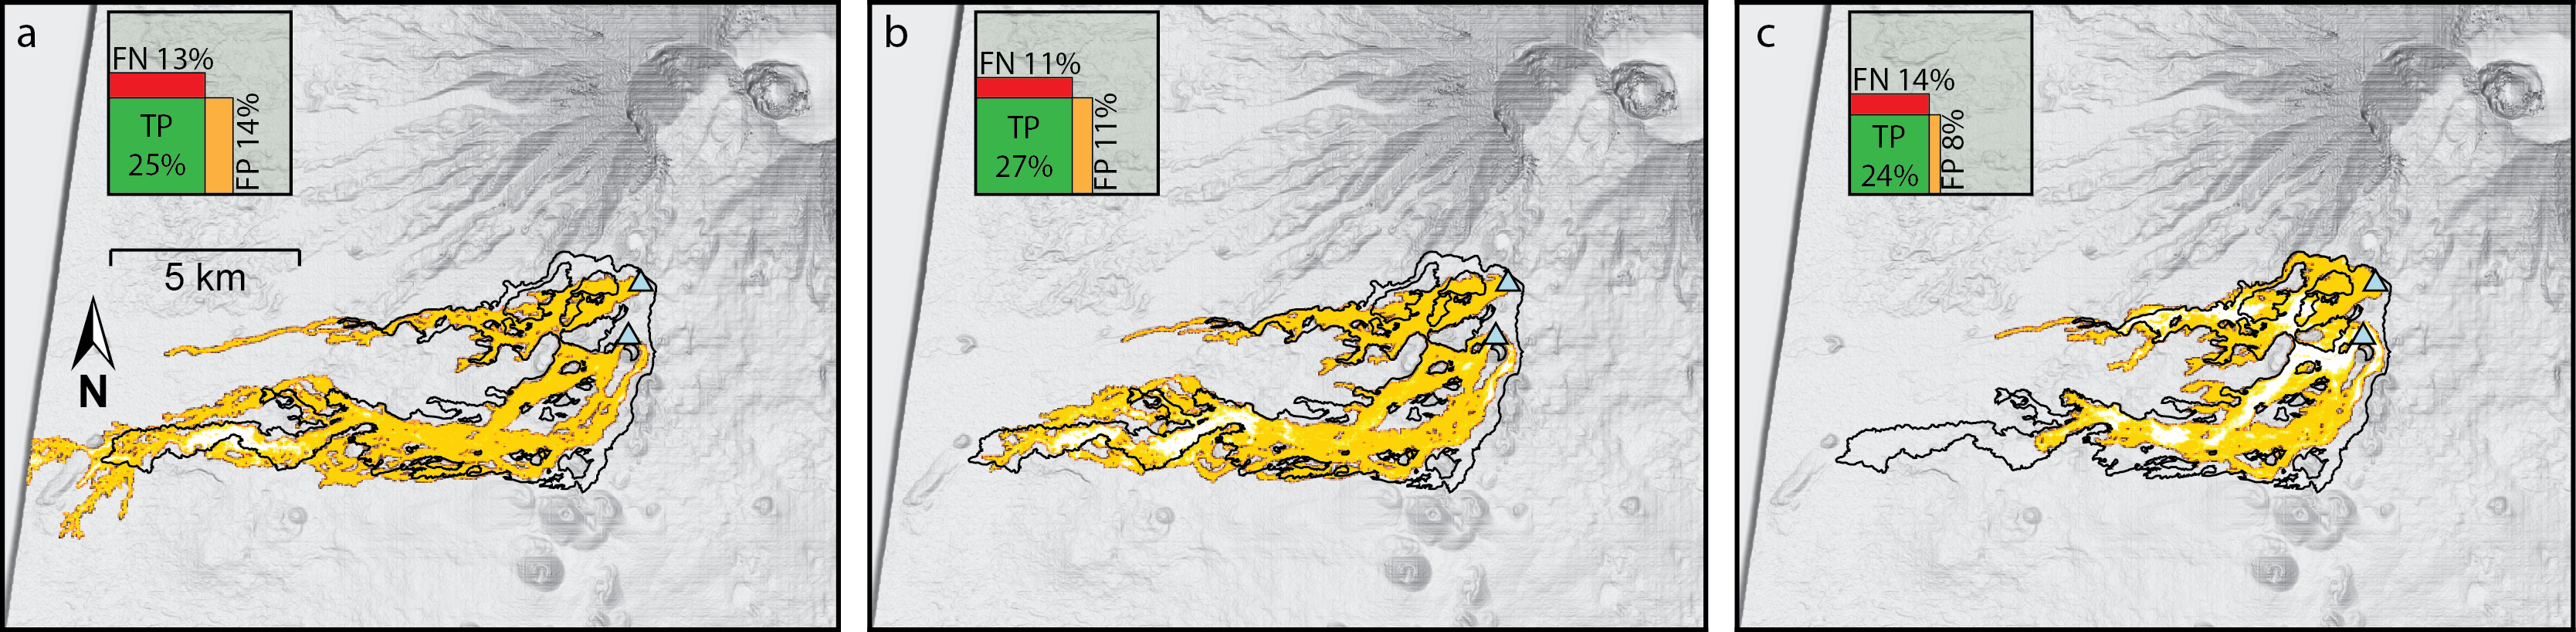
\includegraphics[width=0.9\textwidth]{figures/defense/pulse_examples_300dpi.png}\\[-0.5em]
		\mbox{\footnotesize \textit{Kubanek et al., Bull. Volc., 2015}}
		\end{center}
		\end{columns}
		\end{block}
	%\end{columns}
	}

\iffalse
	\frame{\frametitle{Simulating Lava Flow Emplacement}
	\begin{columns}
	\column{.5\textwidth}
		\begin{block}{}
		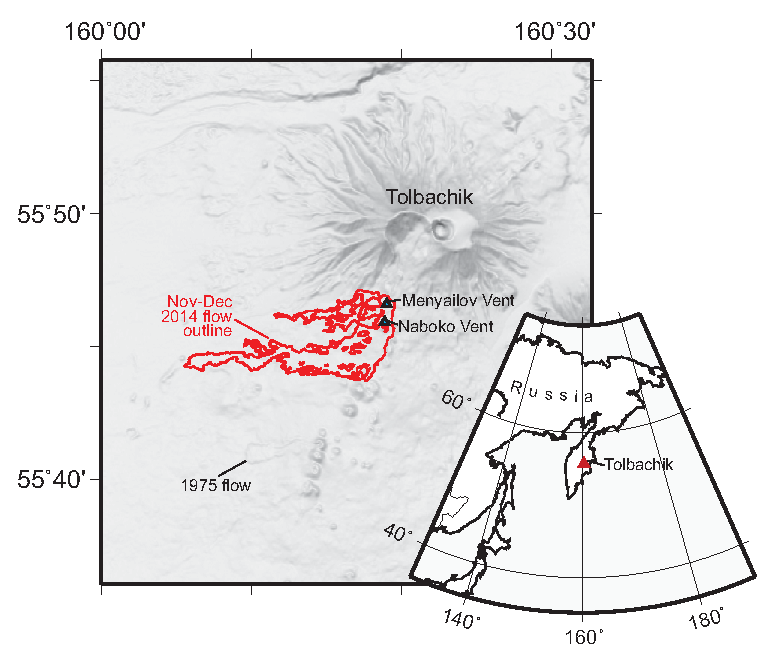
\includegraphics[width=1\textwidth]{figures/chapter-molasses/locator_complete.eps}
		\end{block}
	\column{.5\textwidth}
		\begin{block}{}
		Validation
		\end{block}
	\end{columns}
	}
\fi

%%%%%%%%%%%%%%%%%%%%%%%%%%%%%
%Syria Planum
%
\iffalse
\subsection{Mars Clusters}
	\frame{\frametitle{Syria Planum}
		\begin{columns}
		\column{.5\textwidth}
			\centering
			\includegraphics[width=0.95\textwidth]{figures/chapter-syria_planum/fig1.eps}
		\column{.5\textwidth}
			\begin{block}{Evolution of a Martian volcano cluster}
			\begin{itemize}
				\item Volcanic vents have been cataloged on Syria Planum
				\item Volcanic units are ID'd with geomorphology and embaying flow fronts
				\item Region was active for 900~Ma (3.5-2.6~Ga)
				\item volcanism center shifted with time
			\end{itemize}
			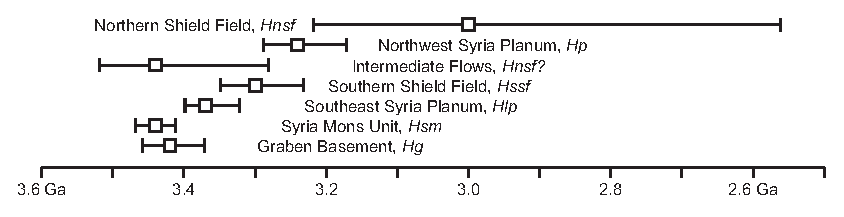
\includegraphics[width=1\textwidth]{figures/chapter-syria_planum/fig2.eps}
			\end{block}
			%% GNUPLOT: LaTeX picture
\setlength{\unitlength}{0.240900pt}
\ifx\plotpoint\undefined\newsavebox{\plotpoint}\fi
\sbox{\plotpoint}{\rule[-0.200pt]{0.400pt}{0.400pt}}%
\begin{picture}(1500,900)(0,0)
\sbox{\plotpoint}{\rule[-0.200pt]{0.400pt}{0.400pt}}%
\put(231.0,131.0){\rule[-0.200pt]{2.409pt}{0.400pt}}
\put(1429.0,131.0){\rule[-0.200pt]{2.409pt}{0.400pt}}
\put(231.0,169.0){\rule[-0.200pt]{2.409pt}{0.400pt}}
\put(1429.0,169.0){\rule[-0.200pt]{2.409pt}{0.400pt}}
\put(231.0,187.0){\rule[-0.200pt]{4.818pt}{0.400pt}}
\put(211,187){\makebox(0,0)[r]{ 1000}}
\put(1419.0,187.0){\rule[-0.200pt]{4.818pt}{0.400pt}}
\put(231.0,243.0){\rule[-0.200pt]{2.409pt}{0.400pt}}
\put(1429.0,243.0){\rule[-0.200pt]{2.409pt}{0.400pt}}
\put(231.0,318.0){\rule[-0.200pt]{2.409pt}{0.400pt}}
\put(1429.0,318.0){\rule[-0.200pt]{2.409pt}{0.400pt}}
\put(231.0,356.0){\rule[-0.200pt]{2.409pt}{0.400pt}}
\put(1429.0,356.0){\rule[-0.200pt]{2.409pt}{0.400pt}}
\put(231.0,374.0){\rule[-0.200pt]{4.818pt}{0.400pt}}
\put(211,374){\makebox(0,0)[r]{ 10000}}
\put(1419.0,374.0){\rule[-0.200pt]{4.818pt}{0.400pt}}
\put(231.0,430.0){\rule[-0.200pt]{2.409pt}{0.400pt}}
\put(1429.0,430.0){\rule[-0.200pt]{2.409pt}{0.400pt}}
\put(231.0,504.0){\rule[-0.200pt]{2.409pt}{0.400pt}}
\put(1429.0,504.0){\rule[-0.200pt]{2.409pt}{0.400pt}}
\put(231.0,542.0){\rule[-0.200pt]{2.409pt}{0.400pt}}
\put(1429.0,542.0){\rule[-0.200pt]{2.409pt}{0.400pt}}
\put(231.0,560.0){\rule[-0.200pt]{4.818pt}{0.400pt}}
\put(211,560){\makebox(0,0)[r]{ 100000}}
\put(1419.0,560.0){\rule[-0.200pt]{4.818pt}{0.400pt}}
\put(231.0,616.0){\rule[-0.200pt]{2.409pt}{0.400pt}}
\put(1429.0,616.0){\rule[-0.200pt]{2.409pt}{0.400pt}}
\put(231.0,691.0){\rule[-0.200pt]{2.409pt}{0.400pt}}
\put(1429.0,691.0){\rule[-0.200pt]{2.409pt}{0.400pt}}
\put(231.0,729.0){\rule[-0.200pt]{2.409pt}{0.400pt}}
\put(1429.0,729.0){\rule[-0.200pt]{2.409pt}{0.400pt}}
\put(231.0,747.0){\rule[-0.200pt]{4.818pt}{0.400pt}}
\put(211,747){\makebox(0,0)[r]{ 1e+06}}
\put(1419.0,747.0){\rule[-0.200pt]{4.818pt}{0.400pt}}
\put(231.0,803.0){\rule[-0.200pt]{2.409pt}{0.400pt}}
\put(1429.0,803.0){\rule[-0.200pt]{2.409pt}{0.400pt}}
\put(231.0,131.0){\rule[-0.200pt]{0.400pt}{2.409pt}}
\put(231.0,849.0){\rule[-0.200pt]{0.400pt}{2.409pt}}
\put(308.0,131.0){\rule[-0.200pt]{0.400pt}{2.409pt}}
\put(308.0,849.0){\rule[-0.200pt]{0.400pt}{2.409pt}}
\put(362.0,131.0){\rule[-0.200pt]{0.400pt}{2.409pt}}
\put(362.0,849.0){\rule[-0.200pt]{0.400pt}{2.409pt}}
\put(404.0,131.0){\rule[-0.200pt]{0.400pt}{2.409pt}}
\put(404.0,849.0){\rule[-0.200pt]{0.400pt}{2.409pt}}
\put(438.0,131.0){\rule[-0.200pt]{0.400pt}{2.409pt}}
\put(438.0,849.0){\rule[-0.200pt]{0.400pt}{2.409pt}}
\put(468.0,131.0){\rule[-0.200pt]{0.400pt}{2.409pt}}
\put(468.0,849.0){\rule[-0.200pt]{0.400pt}{2.409pt}}
\put(493.0,131.0){\rule[-0.200pt]{0.400pt}{2.409pt}}
\put(493.0,849.0){\rule[-0.200pt]{0.400pt}{2.409pt}}
\put(515.0,131.0){\rule[-0.200pt]{0.400pt}{2.409pt}}
\put(515.0,849.0){\rule[-0.200pt]{0.400pt}{2.409pt}}
\put(535.0,131.0){\rule[-0.200pt]{0.400pt}{4.818pt}}
\put(535,90){\makebox(0,0){ 100}}
\put(535.0,839.0){\rule[-0.200pt]{0.400pt}{4.818pt}}
\put(666.0,131.0){\rule[-0.200pt]{0.400pt}{2.409pt}}
\put(666.0,849.0){\rule[-0.200pt]{0.400pt}{2.409pt}}
\put(742.0,131.0){\rule[-0.200pt]{0.400pt}{2.409pt}}
\put(742.0,849.0){\rule[-0.200pt]{0.400pt}{2.409pt}}
\put(797.0,131.0){\rule[-0.200pt]{0.400pt}{2.409pt}}
\put(797.0,849.0){\rule[-0.200pt]{0.400pt}{2.409pt}}
\put(839.0,131.0){\rule[-0.200pt]{0.400pt}{2.409pt}}
\put(839.0,849.0){\rule[-0.200pt]{0.400pt}{2.409pt}}
\put(873.0,131.0){\rule[-0.200pt]{0.400pt}{2.409pt}}
\put(873.0,849.0){\rule[-0.200pt]{0.400pt}{2.409pt}}
\put(902.0,131.0){\rule[-0.200pt]{0.400pt}{2.409pt}}
\put(902.0,849.0){\rule[-0.200pt]{0.400pt}{2.409pt}}
\put(928.0,131.0){\rule[-0.200pt]{0.400pt}{2.409pt}}
\put(928.0,849.0){\rule[-0.200pt]{0.400pt}{2.409pt}}
\put(950.0,131.0){\rule[-0.200pt]{0.400pt}{2.409pt}}
\put(950.0,849.0){\rule[-0.200pt]{0.400pt}{2.409pt}}
\put(970.0,131.0){\rule[-0.200pt]{0.400pt}{4.818pt}}
\put(970,90){\makebox(0,0){ 1000}}
\put(970.0,839.0){\rule[-0.200pt]{0.400pt}{4.818pt}}
\put(1101.0,131.0){\rule[-0.200pt]{0.400pt}{2.409pt}}
\put(1101.0,849.0){\rule[-0.200pt]{0.400pt}{2.409pt}}
\put(1177.0,131.0){\rule[-0.200pt]{0.400pt}{2.409pt}}
\put(1177.0,849.0){\rule[-0.200pt]{0.400pt}{2.409pt}}
\put(1232.0,131.0){\rule[-0.200pt]{0.400pt}{2.409pt}}
\put(1232.0,849.0){\rule[-0.200pt]{0.400pt}{2.409pt}}
\put(1274.0,131.0){\rule[-0.200pt]{0.400pt}{2.409pt}}
\put(1274.0,849.0){\rule[-0.200pt]{0.400pt}{2.409pt}}
\put(1308.0,131.0){\rule[-0.200pt]{0.400pt}{2.409pt}}
\put(1308.0,849.0){\rule[-0.200pt]{0.400pt}{2.409pt}}
\put(1337.0,131.0){\rule[-0.200pt]{0.400pt}{2.409pt}}
\put(1337.0,849.0){\rule[-0.200pt]{0.400pt}{2.409pt}}
\put(1362.0,131.0){\rule[-0.200pt]{0.400pt}{2.409pt}}
\put(1362.0,849.0){\rule[-0.200pt]{0.400pt}{2.409pt}}
\put(1385.0,131.0){\rule[-0.200pt]{0.400pt}{2.409pt}}
\put(1385.0,849.0){\rule[-0.200pt]{0.400pt}{2.409pt}}
\put(1405.0,131.0){\rule[-0.200pt]{0.400pt}{4.818pt}}
\put(1405,90){\makebox(0,0){ 10000}}
\put(1405.0,839.0){\rule[-0.200pt]{0.400pt}{4.818pt}}
\put(231.0,131.0){\rule[-0.200pt]{0.400pt}{175.375pt}}
\put(231.0,131.0){\rule[-0.200pt]{291.007pt}{0.400pt}}
\put(1439.0,131.0){\rule[-0.200pt]{0.400pt}{175.375pt}}
\put(231.0,859.0){\rule[-0.200pt]{291.007pt}{0.400pt}}
\put(30,495){\rotatebox{-270}{\makebox(0,0){2-$sigma$ Cluster Size (km$^2$)}}
}\put(835,29){\makebox(0,0){Vent count in volcano cluster}}
\put(1046,374){\rotatebox{23}{\makebox(0,0)[l]{10 km$^2$ per vent}}
}\put(1046,560){\rotatebox{23}{\makebox(0,0)[l]{100 km$^2$ per vent}}
}\put(873,672){\rotatebox{23}{\makebox(0,0)[l]{1000 km$^2$ per vent}}
}\sbox{\plotpoint}{\rule[-0.500pt]{1.000pt}{1.000pt}}%
\multiput(404,131)(19.085,8.158){7}{\usebox{\plotpoint}}
\multiput(535,187)(19.068,8.197){23}{\usebox{\plotpoint}}
\multiput(970,374)(19.084,8.160){23}{\usebox{\plotpoint}}
\multiput(1405,560)(18.990,8.378){2}{\usebox{\plotpoint}}
\put(1439,575){\usebox{\plotpoint}}
\multiput(231,243)(19.061,8.214){16}{\usebox{\plotpoint}}
\multiput(535,374)(19.084,8.160){23}{\usebox{\plotpoint}}
\multiput(970,560)(19.068,8.197){23}{\usebox{\plotpoint}}
\multiput(1405,747)(19.192,7.903){2}{\usebox{\plotpoint}}
\put(1439,761){\usebox{\plotpoint}}
\multiput(231,430)(19.084,8.161){16}{\usebox{\plotpoint}}
\multiput(535,560)(19.068,8.197){23}{\usebox{\plotpoint}}
\multiput(970,747)(19.085,8.158){14}{\usebox{\plotpoint}}
\put(1232,859){\usebox{\plotpoint}}
\sbox{\plotpoint}{\rule[-0.200pt]{0.400pt}{0.400pt}}%
\put(571,819){\makebox(0,0)[r]{  Earth Clusters}}
\sbox{\plotpoint}{\rule[-0.500pt]{1.000pt}{1.000pt}}%
\put(486,188){\makebox(0,0){$\circ$}}
\put(868,324){\makebox(0,0){$\circ$}}
\put(448,180){\makebox(0,0){$\circ$}}
\put(793,259){\makebox(0,0){$\circ$}}
\put(513,194){\makebox(0,0){$\circ$}}
\put(758,233){\makebox(0,0){$\circ$}}
\put(641,819){\makebox(0,0){$\circ$}}
\sbox{\plotpoint}{\rule[-0.600pt]{1.200pt}{1.200pt}}%
\sbox{\plotpoint}{\rule[-0.200pt]{0.400pt}{0.400pt}}%
\put(571,778){\makebox(0,0)[r]{  Venus Clusters}}
\sbox{\plotpoint}{\rule[-0.600pt]{1.200pt}{1.200pt}}%
\put(767,467){\makebox(0,0){$\bullet$}}
\put(590,364){\makebox(0,0){$\bullet$}}
\put(633,404){\makebox(0,0){$\bullet$}}
\put(735,426){\makebox(0,0){$\bullet$}}
\put(1169,751){\makebox(0,0){$\bullet$}}
\put(1405,777){\makebox(0,0){$\bullet$}}
\put(1201,746){\makebox(0,0){$\bullet$}}
\put(641,778){\makebox(0,0){$\bullet$}}
\sbox{\plotpoint}{\rule[-0.500pt]{1.000pt}{1.000pt}}%
\sbox{\plotpoint}{\rule[-0.200pt]{0.400pt}{0.400pt}}%
\put(571,737){\makebox(0,0)[r]{  Mars Clusters}}
\sbox{\plotpoint}{\rule[-0.500pt]{1.000pt}{1.000pt}}%
\put(301,376){\makebox(0,0){$\ast$}}
\put(513,574){\makebox(0,0){$\ast$}}
\put(715,656){\makebox(0,0){$\ast$}}
\put(641,737){\makebox(0,0){$\ast$}}
\sbox{\plotpoint}{\rule[-0.200pt]{0.400pt}{0.400pt}}%
\put(231.0,131.0){\rule[-0.200pt]{0.400pt}{175.375pt}}
\put(231.0,131.0){\rule[-0.200pt]{291.007pt}{0.400pt}}
\put(1439.0,131.0){\rule[-0.200pt]{0.400pt}{175.375pt}}
\put(231.0,859.0){\rule[-0.200pt]{291.007pt}{0.400pt}}
\end{picture}

		\end{columns}
	}
\fi

\iffalse
	\frame{\frametitle{Syria Planum}
		\begin{columns}
		\column{.46\textwidth}
			\centering
			\includegraphics[width=1\textwidth,clip,trim=1cm 5cm 1cm 1mm]{figures/chapter-syria_planum/fig1.eps}
		\column{.54\textwidth}
			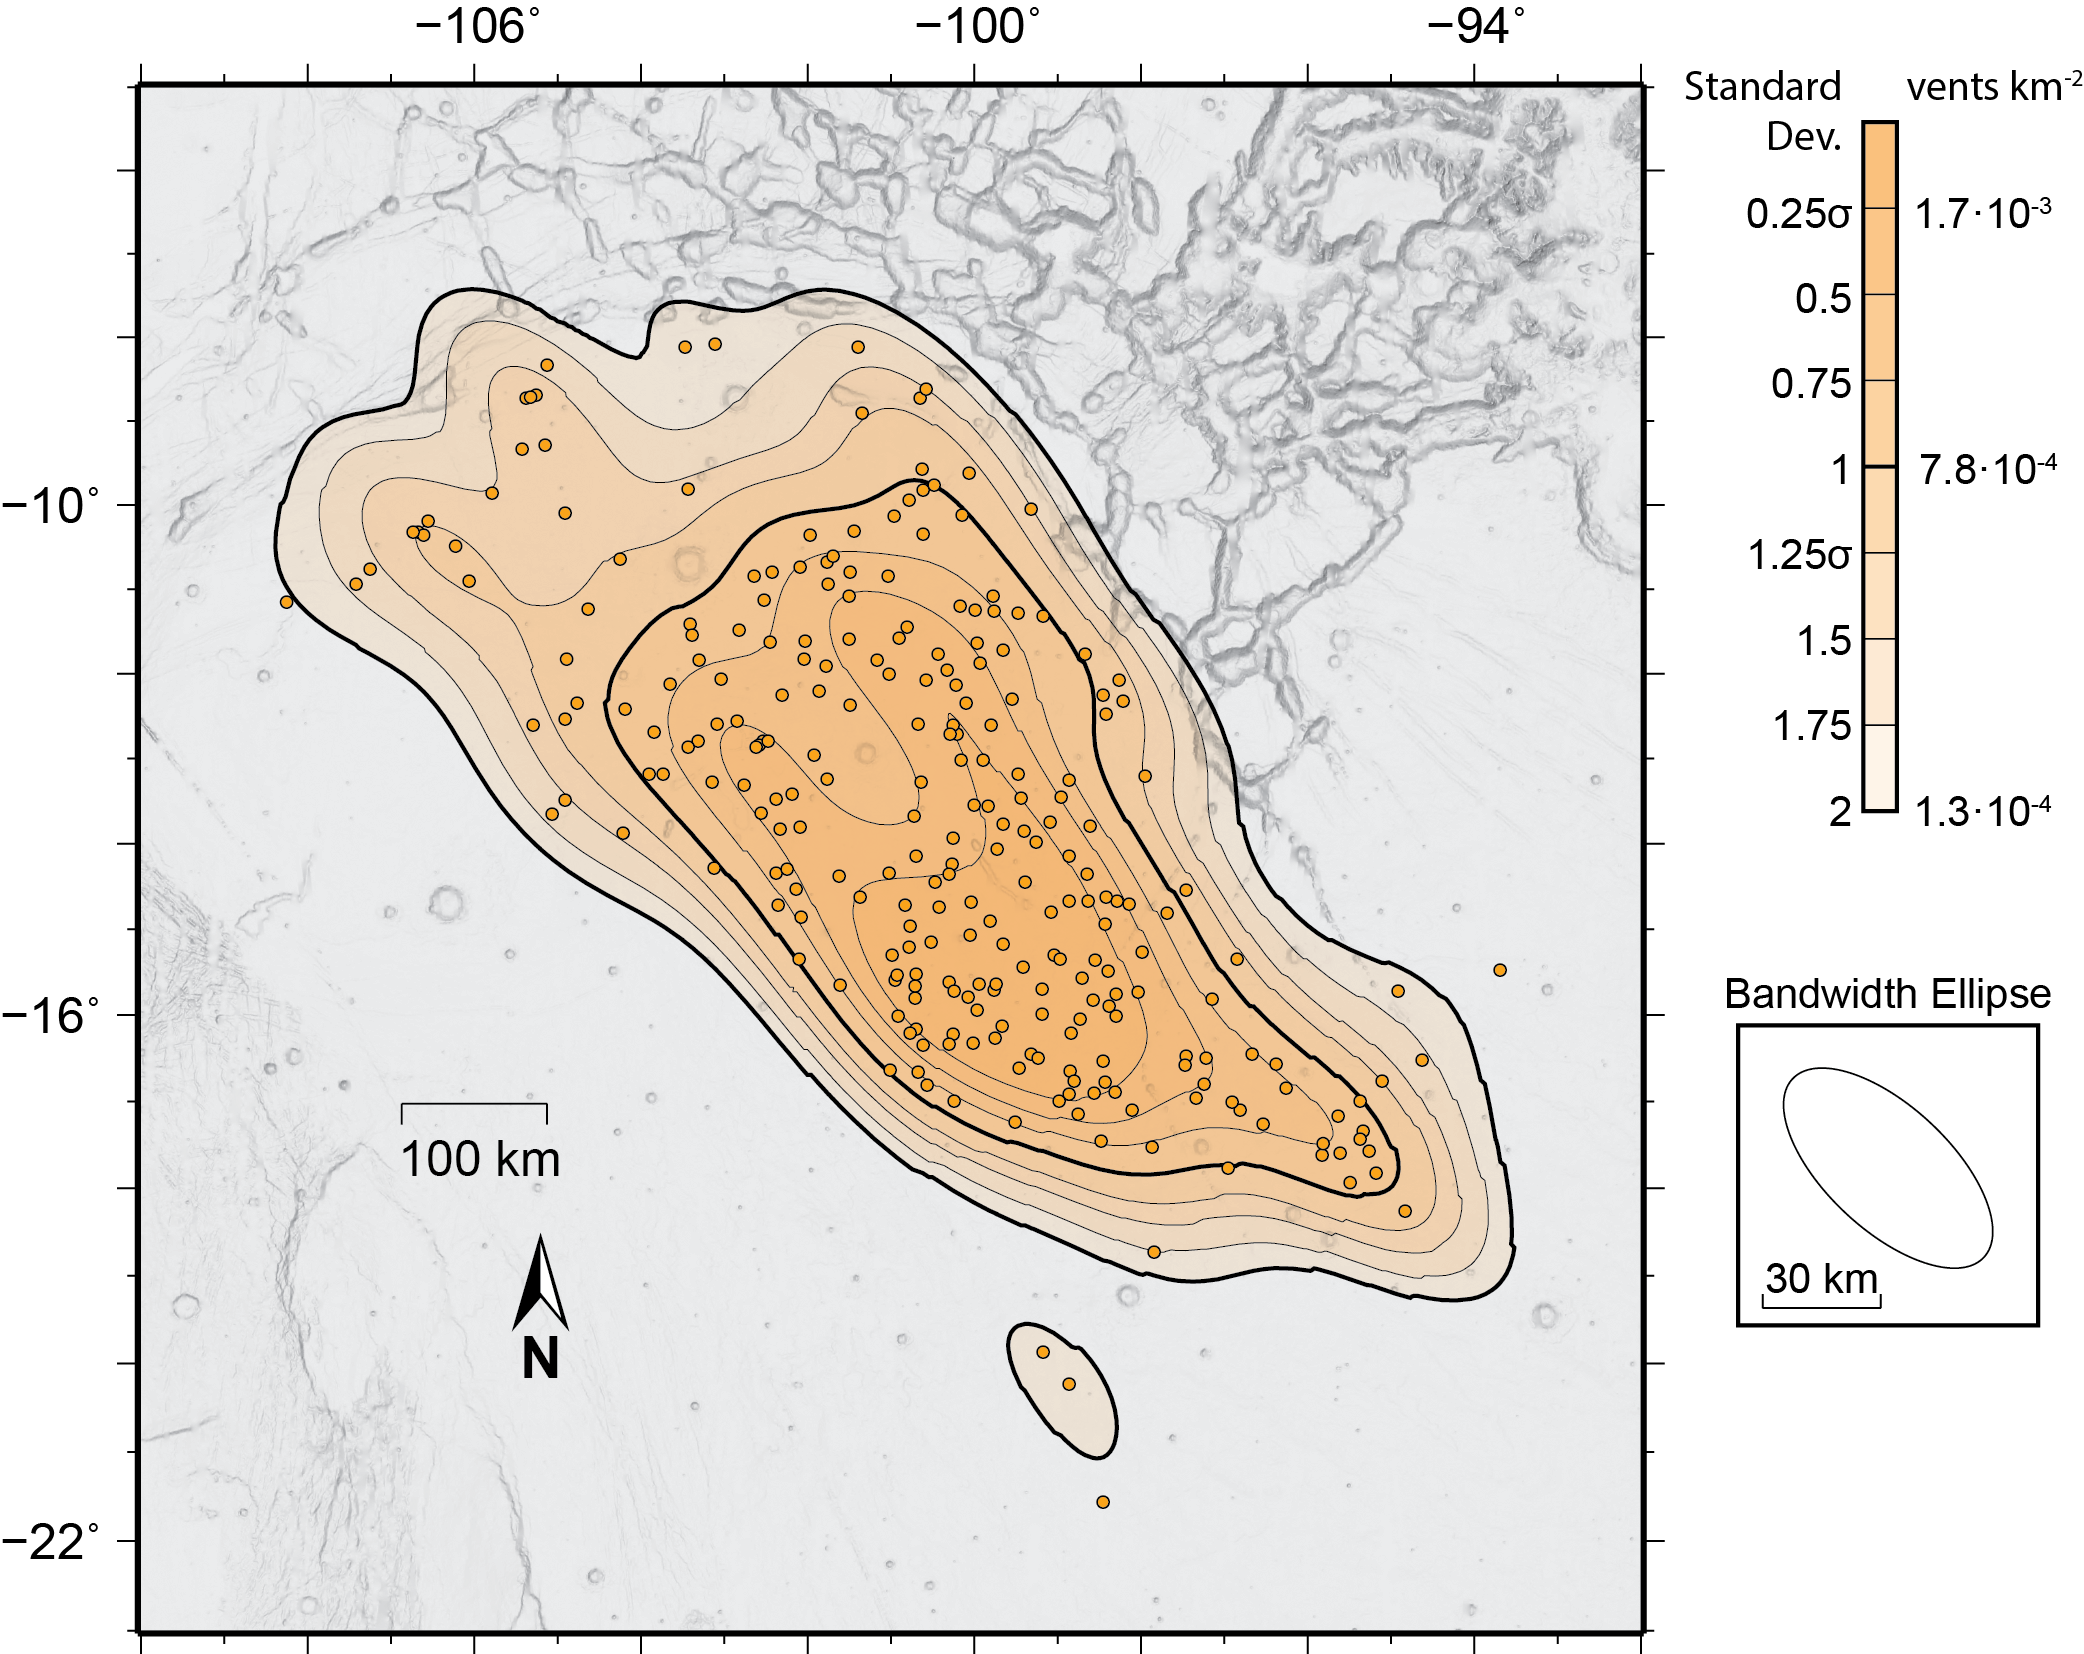
\includegraphics[width=1\textwidth]{figures/chapter-spatial_density/syria_kde_300dpi.png}
			%% GNUPLOT: LaTeX picture
\setlength{\unitlength}{0.240900pt}
\ifx\plotpoint\undefined\newsavebox{\plotpoint}\fi
\sbox{\plotpoint}{\rule[-0.200pt]{0.400pt}{0.400pt}}%
\begin{picture}(1500,900)(0,0)
\sbox{\plotpoint}{\rule[-0.200pt]{0.400pt}{0.400pt}}%
\put(231.0,131.0){\rule[-0.200pt]{2.409pt}{0.400pt}}
\put(1429.0,131.0){\rule[-0.200pt]{2.409pt}{0.400pt}}
\put(231.0,169.0){\rule[-0.200pt]{2.409pt}{0.400pt}}
\put(1429.0,169.0){\rule[-0.200pt]{2.409pt}{0.400pt}}
\put(231.0,187.0){\rule[-0.200pt]{4.818pt}{0.400pt}}
\put(211,187){\makebox(0,0)[r]{ 1000}}
\put(1419.0,187.0){\rule[-0.200pt]{4.818pt}{0.400pt}}
\put(231.0,243.0){\rule[-0.200pt]{2.409pt}{0.400pt}}
\put(1429.0,243.0){\rule[-0.200pt]{2.409pt}{0.400pt}}
\put(231.0,318.0){\rule[-0.200pt]{2.409pt}{0.400pt}}
\put(1429.0,318.0){\rule[-0.200pt]{2.409pt}{0.400pt}}
\put(231.0,356.0){\rule[-0.200pt]{2.409pt}{0.400pt}}
\put(1429.0,356.0){\rule[-0.200pt]{2.409pt}{0.400pt}}
\put(231.0,374.0){\rule[-0.200pt]{4.818pt}{0.400pt}}
\put(211,374){\makebox(0,0)[r]{ 10000}}
\put(1419.0,374.0){\rule[-0.200pt]{4.818pt}{0.400pt}}
\put(231.0,430.0){\rule[-0.200pt]{2.409pt}{0.400pt}}
\put(1429.0,430.0){\rule[-0.200pt]{2.409pt}{0.400pt}}
\put(231.0,504.0){\rule[-0.200pt]{2.409pt}{0.400pt}}
\put(1429.0,504.0){\rule[-0.200pt]{2.409pt}{0.400pt}}
\put(231.0,542.0){\rule[-0.200pt]{2.409pt}{0.400pt}}
\put(1429.0,542.0){\rule[-0.200pt]{2.409pt}{0.400pt}}
\put(231.0,560.0){\rule[-0.200pt]{4.818pt}{0.400pt}}
\put(211,560){\makebox(0,0)[r]{ 100000}}
\put(1419.0,560.0){\rule[-0.200pt]{4.818pt}{0.400pt}}
\put(231.0,616.0){\rule[-0.200pt]{2.409pt}{0.400pt}}
\put(1429.0,616.0){\rule[-0.200pt]{2.409pt}{0.400pt}}
\put(231.0,691.0){\rule[-0.200pt]{2.409pt}{0.400pt}}
\put(1429.0,691.0){\rule[-0.200pt]{2.409pt}{0.400pt}}
\put(231.0,729.0){\rule[-0.200pt]{2.409pt}{0.400pt}}
\put(1429.0,729.0){\rule[-0.200pt]{2.409pt}{0.400pt}}
\put(231.0,747.0){\rule[-0.200pt]{4.818pt}{0.400pt}}
\put(211,747){\makebox(0,0)[r]{ 1e+06}}
\put(1419.0,747.0){\rule[-0.200pt]{4.818pt}{0.400pt}}
\put(231.0,803.0){\rule[-0.200pt]{2.409pt}{0.400pt}}
\put(1429.0,803.0){\rule[-0.200pt]{2.409pt}{0.400pt}}
\put(231.0,131.0){\rule[-0.200pt]{0.400pt}{2.409pt}}
\put(231.0,849.0){\rule[-0.200pt]{0.400pt}{2.409pt}}
\put(308.0,131.0){\rule[-0.200pt]{0.400pt}{2.409pt}}
\put(308.0,849.0){\rule[-0.200pt]{0.400pt}{2.409pt}}
\put(362.0,131.0){\rule[-0.200pt]{0.400pt}{2.409pt}}
\put(362.0,849.0){\rule[-0.200pt]{0.400pt}{2.409pt}}
\put(404.0,131.0){\rule[-0.200pt]{0.400pt}{2.409pt}}
\put(404.0,849.0){\rule[-0.200pt]{0.400pt}{2.409pt}}
\put(438.0,131.0){\rule[-0.200pt]{0.400pt}{2.409pt}}
\put(438.0,849.0){\rule[-0.200pt]{0.400pt}{2.409pt}}
\put(468.0,131.0){\rule[-0.200pt]{0.400pt}{2.409pt}}
\put(468.0,849.0){\rule[-0.200pt]{0.400pt}{2.409pt}}
\put(493.0,131.0){\rule[-0.200pt]{0.400pt}{2.409pt}}
\put(493.0,849.0){\rule[-0.200pt]{0.400pt}{2.409pt}}
\put(515.0,131.0){\rule[-0.200pt]{0.400pt}{2.409pt}}
\put(515.0,849.0){\rule[-0.200pt]{0.400pt}{2.409pt}}
\put(535.0,131.0){\rule[-0.200pt]{0.400pt}{4.818pt}}
\put(535,90){\makebox(0,0){ 100}}
\put(535.0,839.0){\rule[-0.200pt]{0.400pt}{4.818pt}}
\put(666.0,131.0){\rule[-0.200pt]{0.400pt}{2.409pt}}
\put(666.0,849.0){\rule[-0.200pt]{0.400pt}{2.409pt}}
\put(742.0,131.0){\rule[-0.200pt]{0.400pt}{2.409pt}}
\put(742.0,849.0){\rule[-0.200pt]{0.400pt}{2.409pt}}
\put(797.0,131.0){\rule[-0.200pt]{0.400pt}{2.409pt}}
\put(797.0,849.0){\rule[-0.200pt]{0.400pt}{2.409pt}}
\put(839.0,131.0){\rule[-0.200pt]{0.400pt}{2.409pt}}
\put(839.0,849.0){\rule[-0.200pt]{0.400pt}{2.409pt}}
\put(873.0,131.0){\rule[-0.200pt]{0.400pt}{2.409pt}}
\put(873.0,849.0){\rule[-0.200pt]{0.400pt}{2.409pt}}
\put(902.0,131.0){\rule[-0.200pt]{0.400pt}{2.409pt}}
\put(902.0,849.0){\rule[-0.200pt]{0.400pt}{2.409pt}}
\put(928.0,131.0){\rule[-0.200pt]{0.400pt}{2.409pt}}
\put(928.0,849.0){\rule[-0.200pt]{0.400pt}{2.409pt}}
\put(950.0,131.0){\rule[-0.200pt]{0.400pt}{2.409pt}}
\put(950.0,849.0){\rule[-0.200pt]{0.400pt}{2.409pt}}
\put(970.0,131.0){\rule[-0.200pt]{0.400pt}{4.818pt}}
\put(970,90){\makebox(0,0){ 1000}}
\put(970.0,839.0){\rule[-0.200pt]{0.400pt}{4.818pt}}
\put(1101.0,131.0){\rule[-0.200pt]{0.400pt}{2.409pt}}
\put(1101.0,849.0){\rule[-0.200pt]{0.400pt}{2.409pt}}
\put(1177.0,131.0){\rule[-0.200pt]{0.400pt}{2.409pt}}
\put(1177.0,849.0){\rule[-0.200pt]{0.400pt}{2.409pt}}
\put(1232.0,131.0){\rule[-0.200pt]{0.400pt}{2.409pt}}
\put(1232.0,849.0){\rule[-0.200pt]{0.400pt}{2.409pt}}
\put(1274.0,131.0){\rule[-0.200pt]{0.400pt}{2.409pt}}
\put(1274.0,849.0){\rule[-0.200pt]{0.400pt}{2.409pt}}
\put(1308.0,131.0){\rule[-0.200pt]{0.400pt}{2.409pt}}
\put(1308.0,849.0){\rule[-0.200pt]{0.400pt}{2.409pt}}
\put(1337.0,131.0){\rule[-0.200pt]{0.400pt}{2.409pt}}
\put(1337.0,849.0){\rule[-0.200pt]{0.400pt}{2.409pt}}
\put(1362.0,131.0){\rule[-0.200pt]{0.400pt}{2.409pt}}
\put(1362.0,849.0){\rule[-0.200pt]{0.400pt}{2.409pt}}
\put(1385.0,131.0){\rule[-0.200pt]{0.400pt}{2.409pt}}
\put(1385.0,849.0){\rule[-0.200pt]{0.400pt}{2.409pt}}
\put(1405.0,131.0){\rule[-0.200pt]{0.400pt}{4.818pt}}
\put(1405,90){\makebox(0,0){ 10000}}
\put(1405.0,839.0){\rule[-0.200pt]{0.400pt}{4.818pt}}
\put(231.0,131.0){\rule[-0.200pt]{0.400pt}{175.375pt}}
\put(231.0,131.0){\rule[-0.200pt]{291.007pt}{0.400pt}}
\put(1439.0,131.0){\rule[-0.200pt]{0.400pt}{175.375pt}}
\put(231.0,859.0){\rule[-0.200pt]{291.007pt}{0.400pt}}
\put(30,495){\rotatebox{-270}{\makebox(0,0){2-$sigma$ Cluster Size (km$^2$)}}
}\put(835,29){\makebox(0,0){Vent count in volcano cluster}}
\put(1046,374){\rotatebox{23}{\makebox(0,0)[l]{10 km$^2$ per vent}}
}\put(1046,560){\rotatebox{23}{\makebox(0,0)[l]{100 km$^2$ per vent}}
}\put(873,672){\rotatebox{23}{\makebox(0,0)[l]{1000 km$^2$ per vent}}
}\sbox{\plotpoint}{\rule[-0.500pt]{1.000pt}{1.000pt}}%
\multiput(404,131)(19.085,8.158){7}{\usebox{\plotpoint}}
\multiput(535,187)(19.068,8.197){23}{\usebox{\plotpoint}}
\multiput(970,374)(19.084,8.160){23}{\usebox{\plotpoint}}
\multiput(1405,560)(18.990,8.378){2}{\usebox{\plotpoint}}
\put(1439,575){\usebox{\plotpoint}}
\multiput(231,243)(19.061,8.214){16}{\usebox{\plotpoint}}
\multiput(535,374)(19.084,8.160){23}{\usebox{\plotpoint}}
\multiput(970,560)(19.068,8.197){23}{\usebox{\plotpoint}}
\multiput(1405,747)(19.192,7.903){2}{\usebox{\plotpoint}}
\put(1439,761){\usebox{\plotpoint}}
\multiput(231,430)(19.084,8.161){16}{\usebox{\plotpoint}}
\multiput(535,560)(19.068,8.197){23}{\usebox{\plotpoint}}
\multiput(970,747)(19.085,8.158){14}{\usebox{\plotpoint}}
\put(1232,859){\usebox{\plotpoint}}
\sbox{\plotpoint}{\rule[-0.200pt]{0.400pt}{0.400pt}}%
\put(571,819){\makebox(0,0)[r]{  Earth Clusters}}
\sbox{\plotpoint}{\rule[-0.500pt]{1.000pt}{1.000pt}}%
\put(486,188){\makebox(0,0){$\circ$}}
\put(868,324){\makebox(0,0){$\circ$}}
\put(448,180){\makebox(0,0){$\circ$}}
\put(793,259){\makebox(0,0){$\circ$}}
\put(513,194){\makebox(0,0){$\circ$}}
\put(758,233){\makebox(0,0){$\circ$}}
\put(641,819){\makebox(0,0){$\circ$}}
\sbox{\plotpoint}{\rule[-0.600pt]{1.200pt}{1.200pt}}%
\sbox{\plotpoint}{\rule[-0.200pt]{0.400pt}{0.400pt}}%
\put(571,778){\makebox(0,0)[r]{  Venus Clusters}}
\sbox{\plotpoint}{\rule[-0.600pt]{1.200pt}{1.200pt}}%
\put(767,467){\makebox(0,0){$\bullet$}}
\put(590,364){\makebox(0,0){$\bullet$}}
\put(633,404){\makebox(0,0){$\bullet$}}
\put(735,426){\makebox(0,0){$\bullet$}}
\put(1169,751){\makebox(0,0){$\bullet$}}
\put(1405,777){\makebox(0,0){$\bullet$}}
\put(1201,746){\makebox(0,0){$\bullet$}}
\put(641,778){\makebox(0,0){$\bullet$}}
\sbox{\plotpoint}{\rule[-0.500pt]{1.000pt}{1.000pt}}%
\sbox{\plotpoint}{\rule[-0.200pt]{0.400pt}{0.400pt}}%
\put(571,737){\makebox(0,0)[r]{  Mars Clusters}}
\sbox{\plotpoint}{\rule[-0.500pt]{1.000pt}{1.000pt}}%
\put(301,376){\makebox(0,0){$\ast$}}
\put(513,574){\makebox(0,0){$\ast$}}
\put(715,656){\makebox(0,0){$\ast$}}
\put(641,737){\makebox(0,0){$\ast$}}
\sbox{\plotpoint}{\rule[-0.200pt]{0.400pt}{0.400pt}}%
\put(231.0,131.0){\rule[-0.200pt]{0.400pt}{175.375pt}}
\put(231.0,131.0){\rule[-0.200pt]{291.007pt}{0.400pt}}
\put(1439.0,131.0){\rule[-0.200pt]{0.400pt}{175.375pt}}
\put(231.0,859.0){\rule[-0.200pt]{291.007pt}{0.400pt}}
\end{picture}

		\end{columns}
	}
\fi

%%%%%%%%%%%%%%%%%%%%%%%%%%%%%%%%%%%%%%%%%%%%%%%%%%%%%%%%%%
%%   ARSIA MONS   %%
%%%%%%%%%%%%%%%%%%%%%%%%%%%%%%%%%%%%%%%
%%%%%%%%%%%%%%%%%%%%%%%%%%%%%%
%%%%%%%%%%%%%%%%%%%%%
%%%%%%%%%%%%

\section{Arsia Mons Volcanic Field}
	\frame{\frametitle{Distributed Volcanism of the Tharsis Volcanic Province}
		\begin{columns}
		\column{0.48\textwidth}
		\centering
		\includegraphics[width=1\textwidth]{figures/defense/catalog_whole_planet_150dpi}
		\column{0.52\textwidth}
		\begin{block}{Tharsis Vent Catalog}
			\begin{itemize}
				\item $>$1,000 small volcanic vents cataloged \mbox{\tiny (Richardson et al., \textit{JVGR}, 2013}, \mbox{\tiny Bleacher et al., \textit{JVGR}, 2009)}
				\item Groups of vents form isolated clusters
			\end{itemize}
		\end{block}
		\begin{block}{Research Questions}
			\begin{itemize}
				\item How does distributed-style volcanism occur over time and space in Tharsis?
				\item How do volcanic fields relate to the larger volcanoes on Mars?
			\end{itemize}
		\end{block}
		\end{columns}
	}

	\frame{\frametitle{Arsia Mons Overview}
		\begin{block}{Arsia Mons}
		\begin{columns}
		\column{0.4\textwidth}
		\begin{itemize}
			\item Large (1.5$\cdot$10$^6$~km$^3$) shield volcano with 110~km diameter caldera
			\item A cluster of volcanic vents lay in the caldera!
		\end{itemize}\\[-1em]
		\begin{center}\textbf{Motivation}\end{center}\\[-1em]
		What are the recurrence rate of volcanism and delivery rate of magma to the surface?
		\column{0.6\textwidth}
		\centering
		\includegraphics[width=0.9\textwidth]{figures/defense/arsia_overview.jpg}
		\end{columns}
		\end{block}
	}
	
	\frame{\frametitle{Arsia Mons Overview}
		\begin{block}{Recurrence Rate and Magma Delivery Rate}
		\begin{columns}
		\column{0.6\textwidth}
		\begin{equation*}
			\text{Recurrence Rate} = \frac{\text{Number of Events - 1}}{\text{Time elapsed}}
		\end{equation*}
		\begin{equation*}
			\text{Delivery Rate} = \frac{\text{Total Volume}}{\text{Number of Events}}\times\text{Recurrence Rate}
		\end{equation*}
		
		\begin{itemize}
		\item Lavas from these vents can be mapped to estimate volume and timing of emplacement
		\end{itemize}
		
		\column{0.4\textwidth}
		\centering
		\includegraphics[width=0.9\textwidth]{figures/defense/arsia_overview.jpg}
		\end{columns}
		\end{block}
	}


\subsection{Methods}
	\frame{\frametitle{Mapping Volcanic Vents}
		\centering
		\includegraphics[width=0.82\textwidth]{figures/defense/V19-V23_view-nooutlines_300dpi.png}\\[-0.5em]
		\mbox{\tiny \textit{CTX Image: G10\_022160\_1710\_XN\_09S120W (NASA/JPL-Caltech/MSSS)}}
	}

	\frame{\frametitle{Mapping Lava Flows}
		\centering
		\includegraphics[width=0.82\textwidth]{figures/defense/V19-V23_view-outlines_300dpi.png}\\[-0.5em]
		\mbox{\tiny \textit{CTX Image: G10\_022160\_1710\_XN\_09S120W (NASA/JPL-Caltech/MSSS)}}
	}

	\frame{\frametitle{Lava Flow Map of Arsia Mons' Caldera}
		\begin{columns}
		\column{0.5\textwidth}
			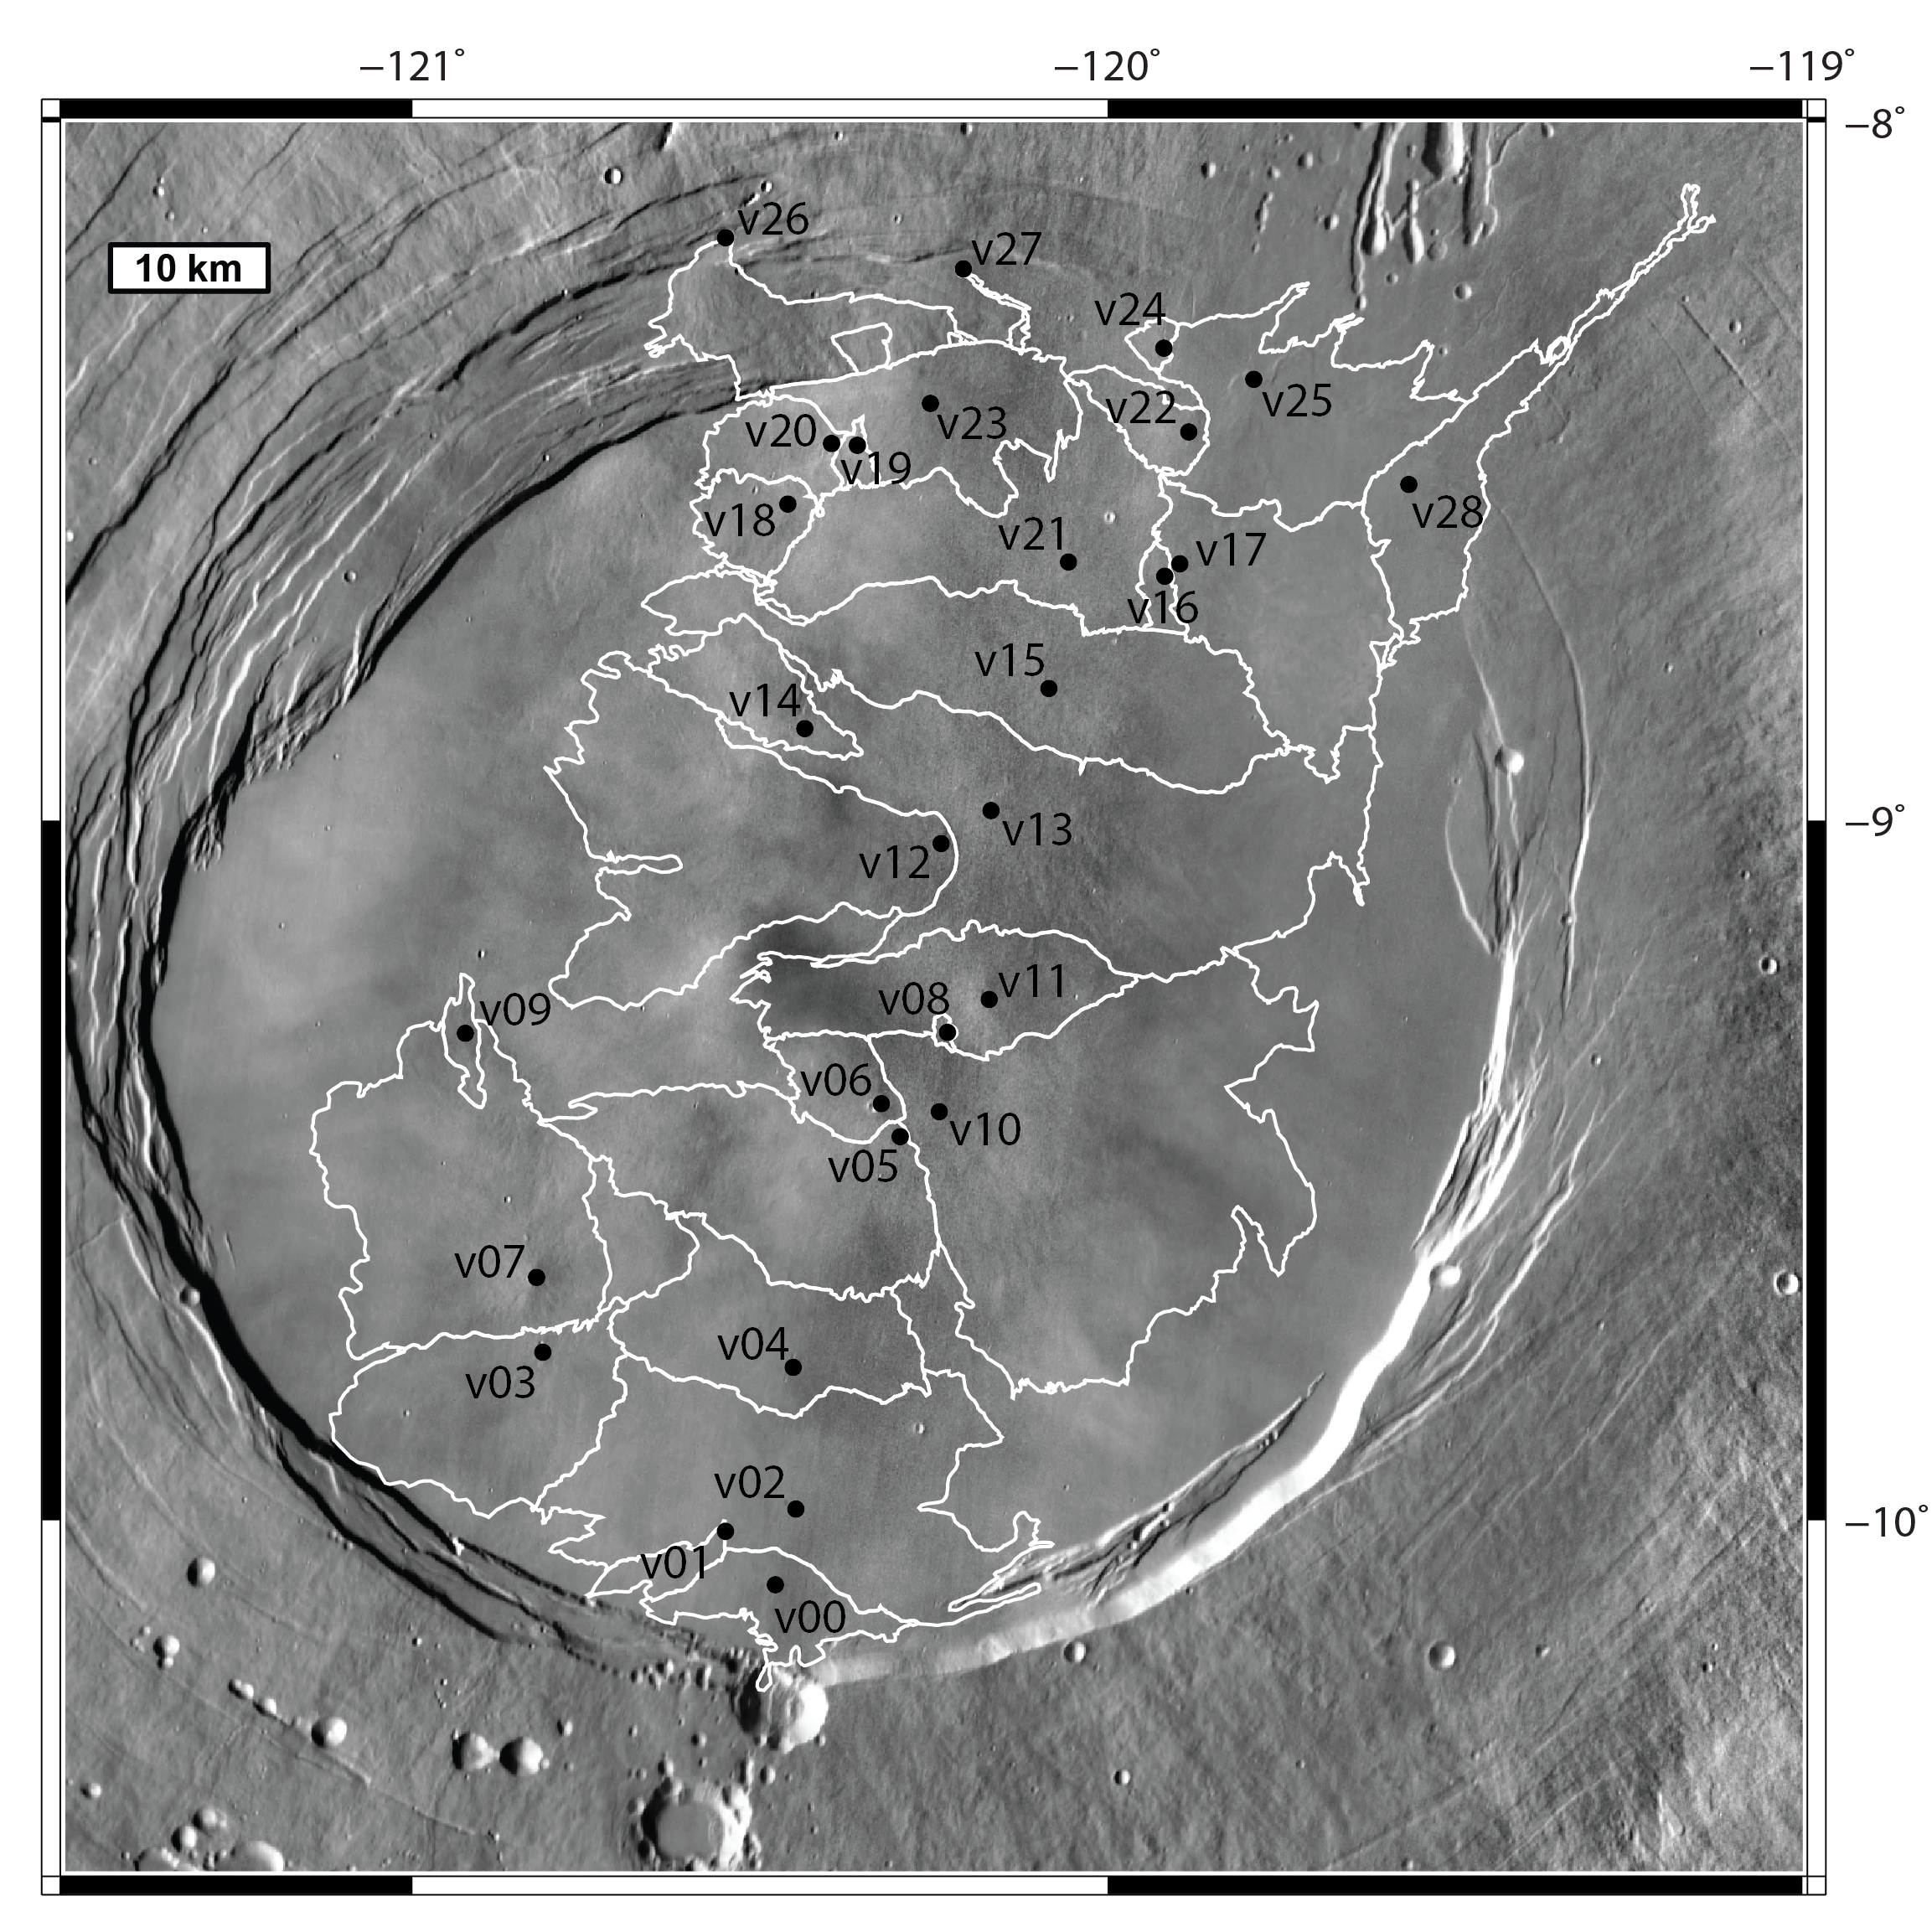
\includegraphics[width=1\textwidth]{figures/defense/arsia_maponly_300dpi}
		\column{0.5\textwidth}
			\begin{block}{Mapping results}
			\begin{itemize}
			\item 29 vents are cataloged, each with long lava flows
			\item Lava flow areas are 10s--100s km$^2$
			\item Flow thicknesses assumed to be 10--80~m {\scriptsize (Mouginis-Mark \& Rowland, Icarus, 2008)}
			\item From this, volumes estimates range from 10$^{-2}$--70~km$^3$
			\end{itemize}
			\end{block}
		\end{columns}
	}


	\frame{\frametitle{Ages: Crater Counting}
	\begin{columns}
	\column{0.75\textwidth}
		\begin{tikzpicture}
			\node (img1) {\includegraphics[width=1\textwidth]{figures/defense/V19-V23_view-outlines_300dpi.png}};
			%\pause
			\node (img2) at (img1.center) [xshift=2cm] {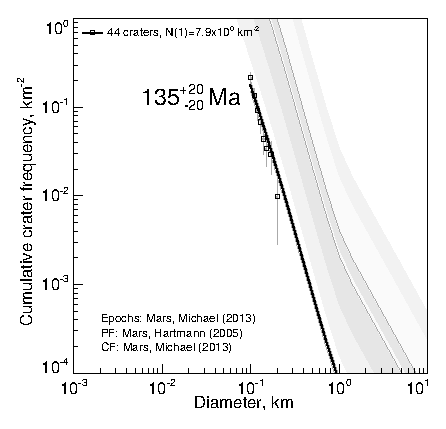
\includegraphics[width=0.27\textwidth]{figures/defense/120-25W_08-40S_100m_cum_fordefense.eps}};
		\end{tikzpicture}\\[-1em]
		%\includegraphics[width=0.82\textwidth]{figures/defense/V19-V23_view-outlines_300dpi.png}\\[-0.5em]
		\mbox{\tiny \textit{CTX Image: G10\_022160\_1710\_XN\_09S120W (NASA/JPL-Caltech/MSSS)}}
	\column{0.25\textwidth}
	\begin{block}{}
	\centering
	Impact craters on each flow are cataloged\\[1.5em]
	More craters generally indicates older age\\[1.5em]
	Ages and uncertainties modeled in \textit{craterstats2} {\scriptsize(Michael, \textit{Icarus}, 2013)}
	\end{block}
	\end{columns}
	}

	\frame{\frametitle{Ages: Crater Counting}
	\begin{block}{}
		Ages of flow emplacement are modeled as Normal Distributions
		\begin{itemize}
			\item Estimated age from \textit{craterstats2} is used as the Mean Value
			\item Age Uncertainty is Standard Deviation
		\end{itemize}
		\begin{columns}
			\column{0.45\textwidth}
				\centering
				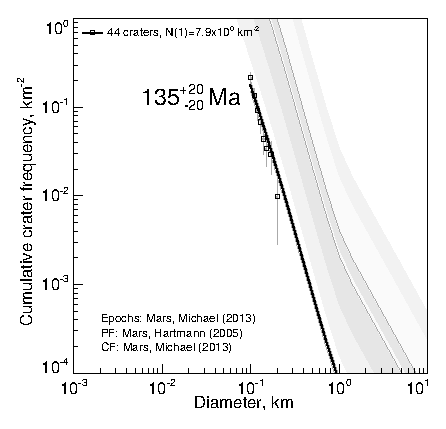
\includegraphics[width=0.8\textwidth]{figures/defense/120-25W_08-40S_100m_cum_fordefense.eps}
			\column{0.1\textwidth}
				\centering
				{\Huge$\Rightarrow$}
			\column{0.45\textwidth}
				\centering
				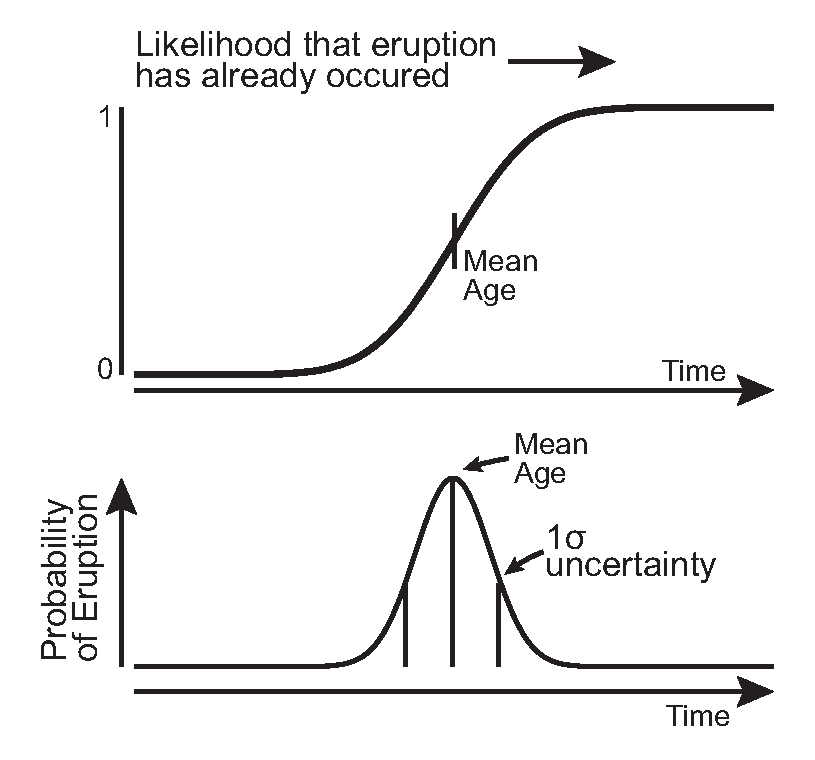
\includegraphics[width=0.8\textwidth]{figures/defense/crater_cdfmodel.eps}
		\end{columns}
	\end{block}
	}

	\frame{\frametitle{Ages: Stratigraphy}
	\begin{columns}
	\column{0.75\textwidth}
	\includegraphics[width=1\textwidth]{figures/defense/V19-V23_view-outlines-HL_300dpi.png}\\[-0.5em]
	\mbox{\tiny \textit{CTX Image: G10\_022160\_1710\_XN\_09S120W (NASA/JPL-Caltech/MSSS)}}
	\column{0.25\textwidth}
	%Stratigraphy Web Key
	\begin{block}{}
	\centering
	Stratigraphic relationships relatively date events.\\[1em]
	Lava from v19 overlies v23 lavas\\[1em]
	\textit{Graphical Form}:\\[-0.2em]
	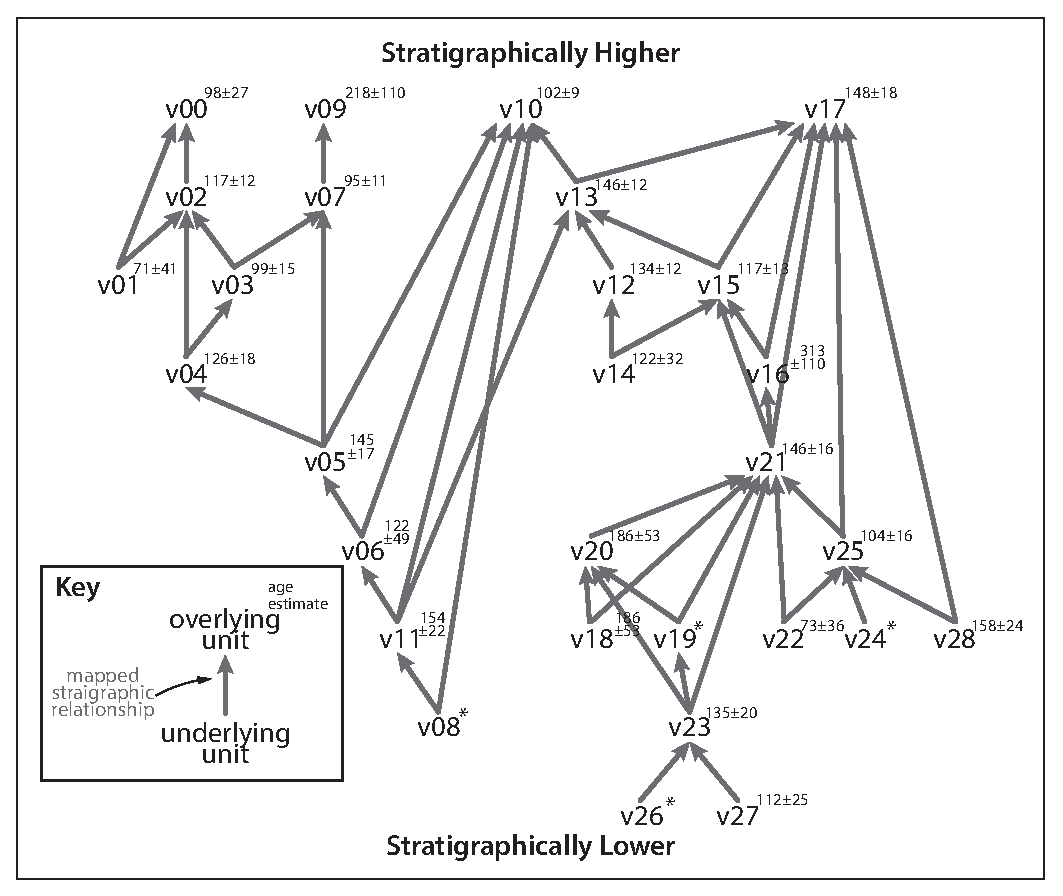
\includegraphics[width=0.8\textwidth,clip,trim=0.2cm 1cm 11.8cm 9.2cm]{figures/defense/stratigraphy_web.eps} %
	\end{block}
	\end{columns}
	}
	
\iffalse
	\frame{\frametitle{Ages: Stratigraphy}
	\begin{columns}
	\column{0.8\textwidth}
	\includegraphics[width=1\textwidth]{figures/defense/V19-V23_view-nooutlines_300dpi.png}\\[-0.5em]
	\mbox{\tiny \textit{CTX Image: G10\_022160\_1710\_XN\_09S120W (NASA/JPL-Caltech/MSSS)}}
	\column{0.2\textwidth}
	%Stratigraphy Web Key
	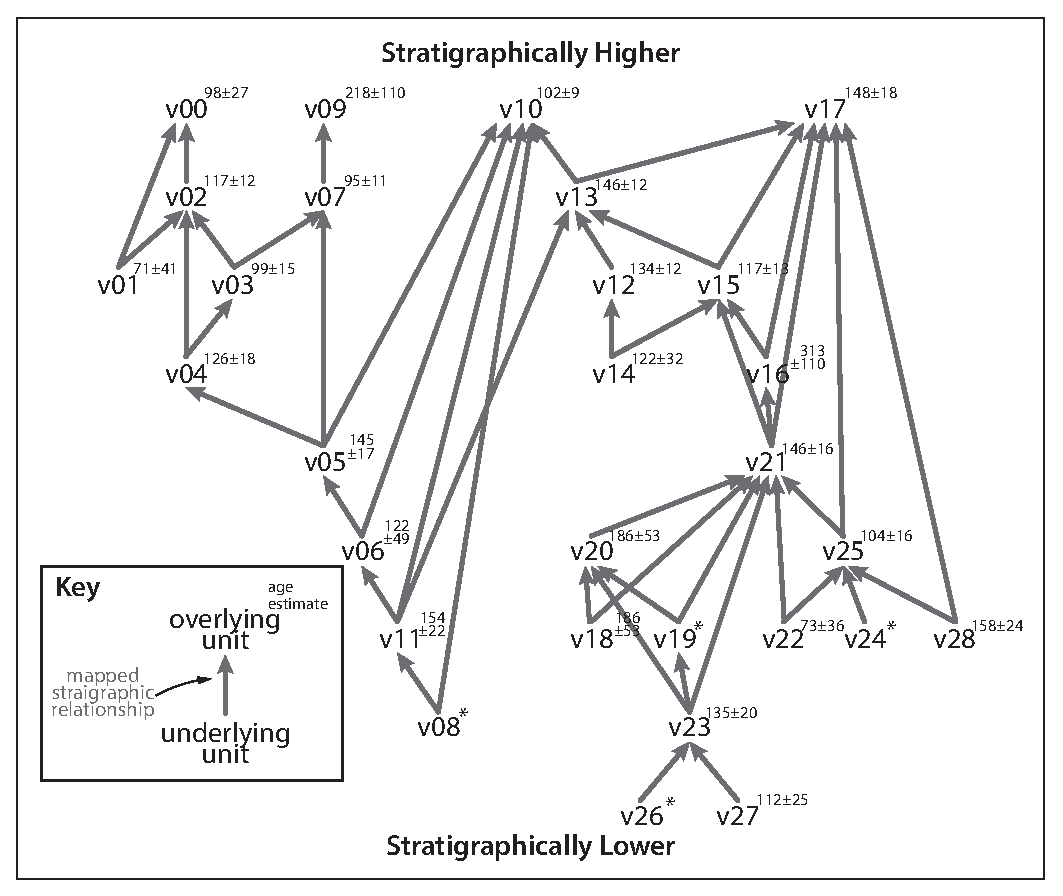
\includegraphics[width=1\textwidth,clip,trim=0.2cm 1cm 11.8cm 9.2cm]{figures/defense/stratigraphy_web.eps} %
	\end{columns}
	}
\fi

	\frame{\frametitle{Combined Age Information}
	\begin{columns}
	%Stratigraphy Web
	\column{0.5\textwidth}
		\begin{block}{Stratigraphy ``Web''}
		\centering
		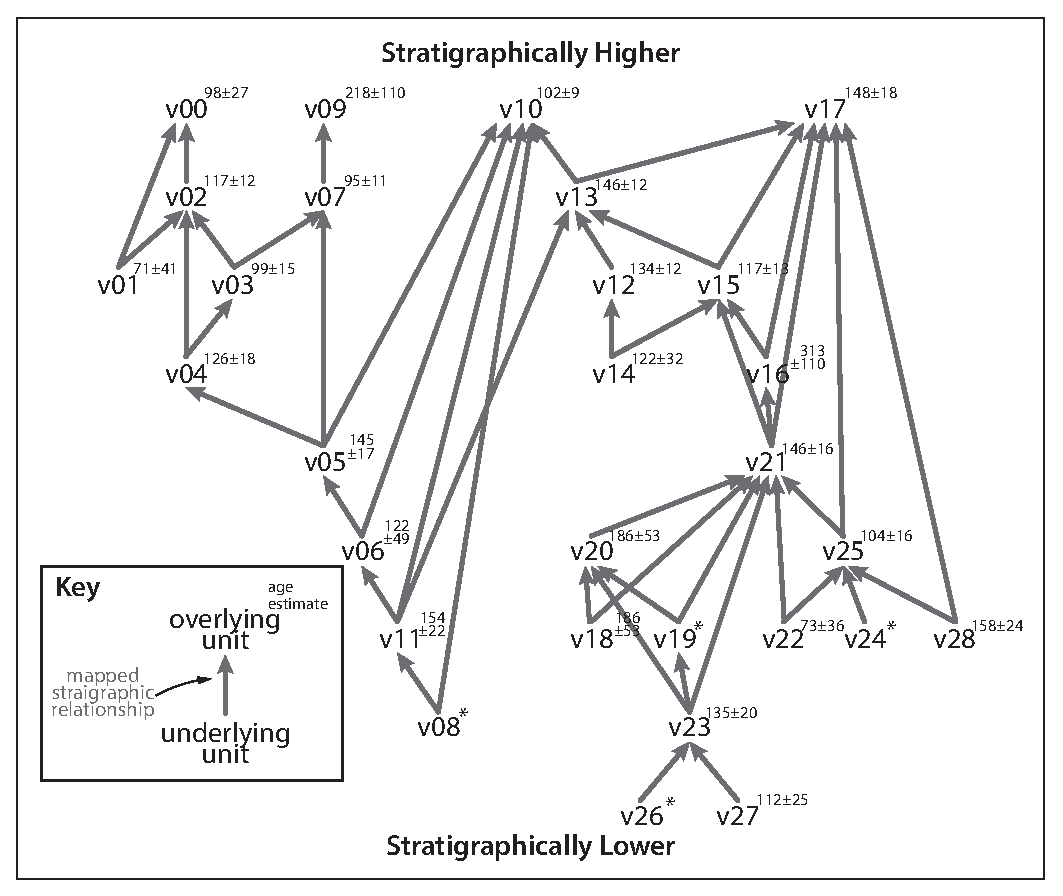
\includegraphics[width=1\textwidth]{figures/defense/stratigraphy_web.eps} %
		\end{block}
	\column{0.5\textwidth}
		\centering
	%Stratigraphy Map - Change to get rid of volume dots
	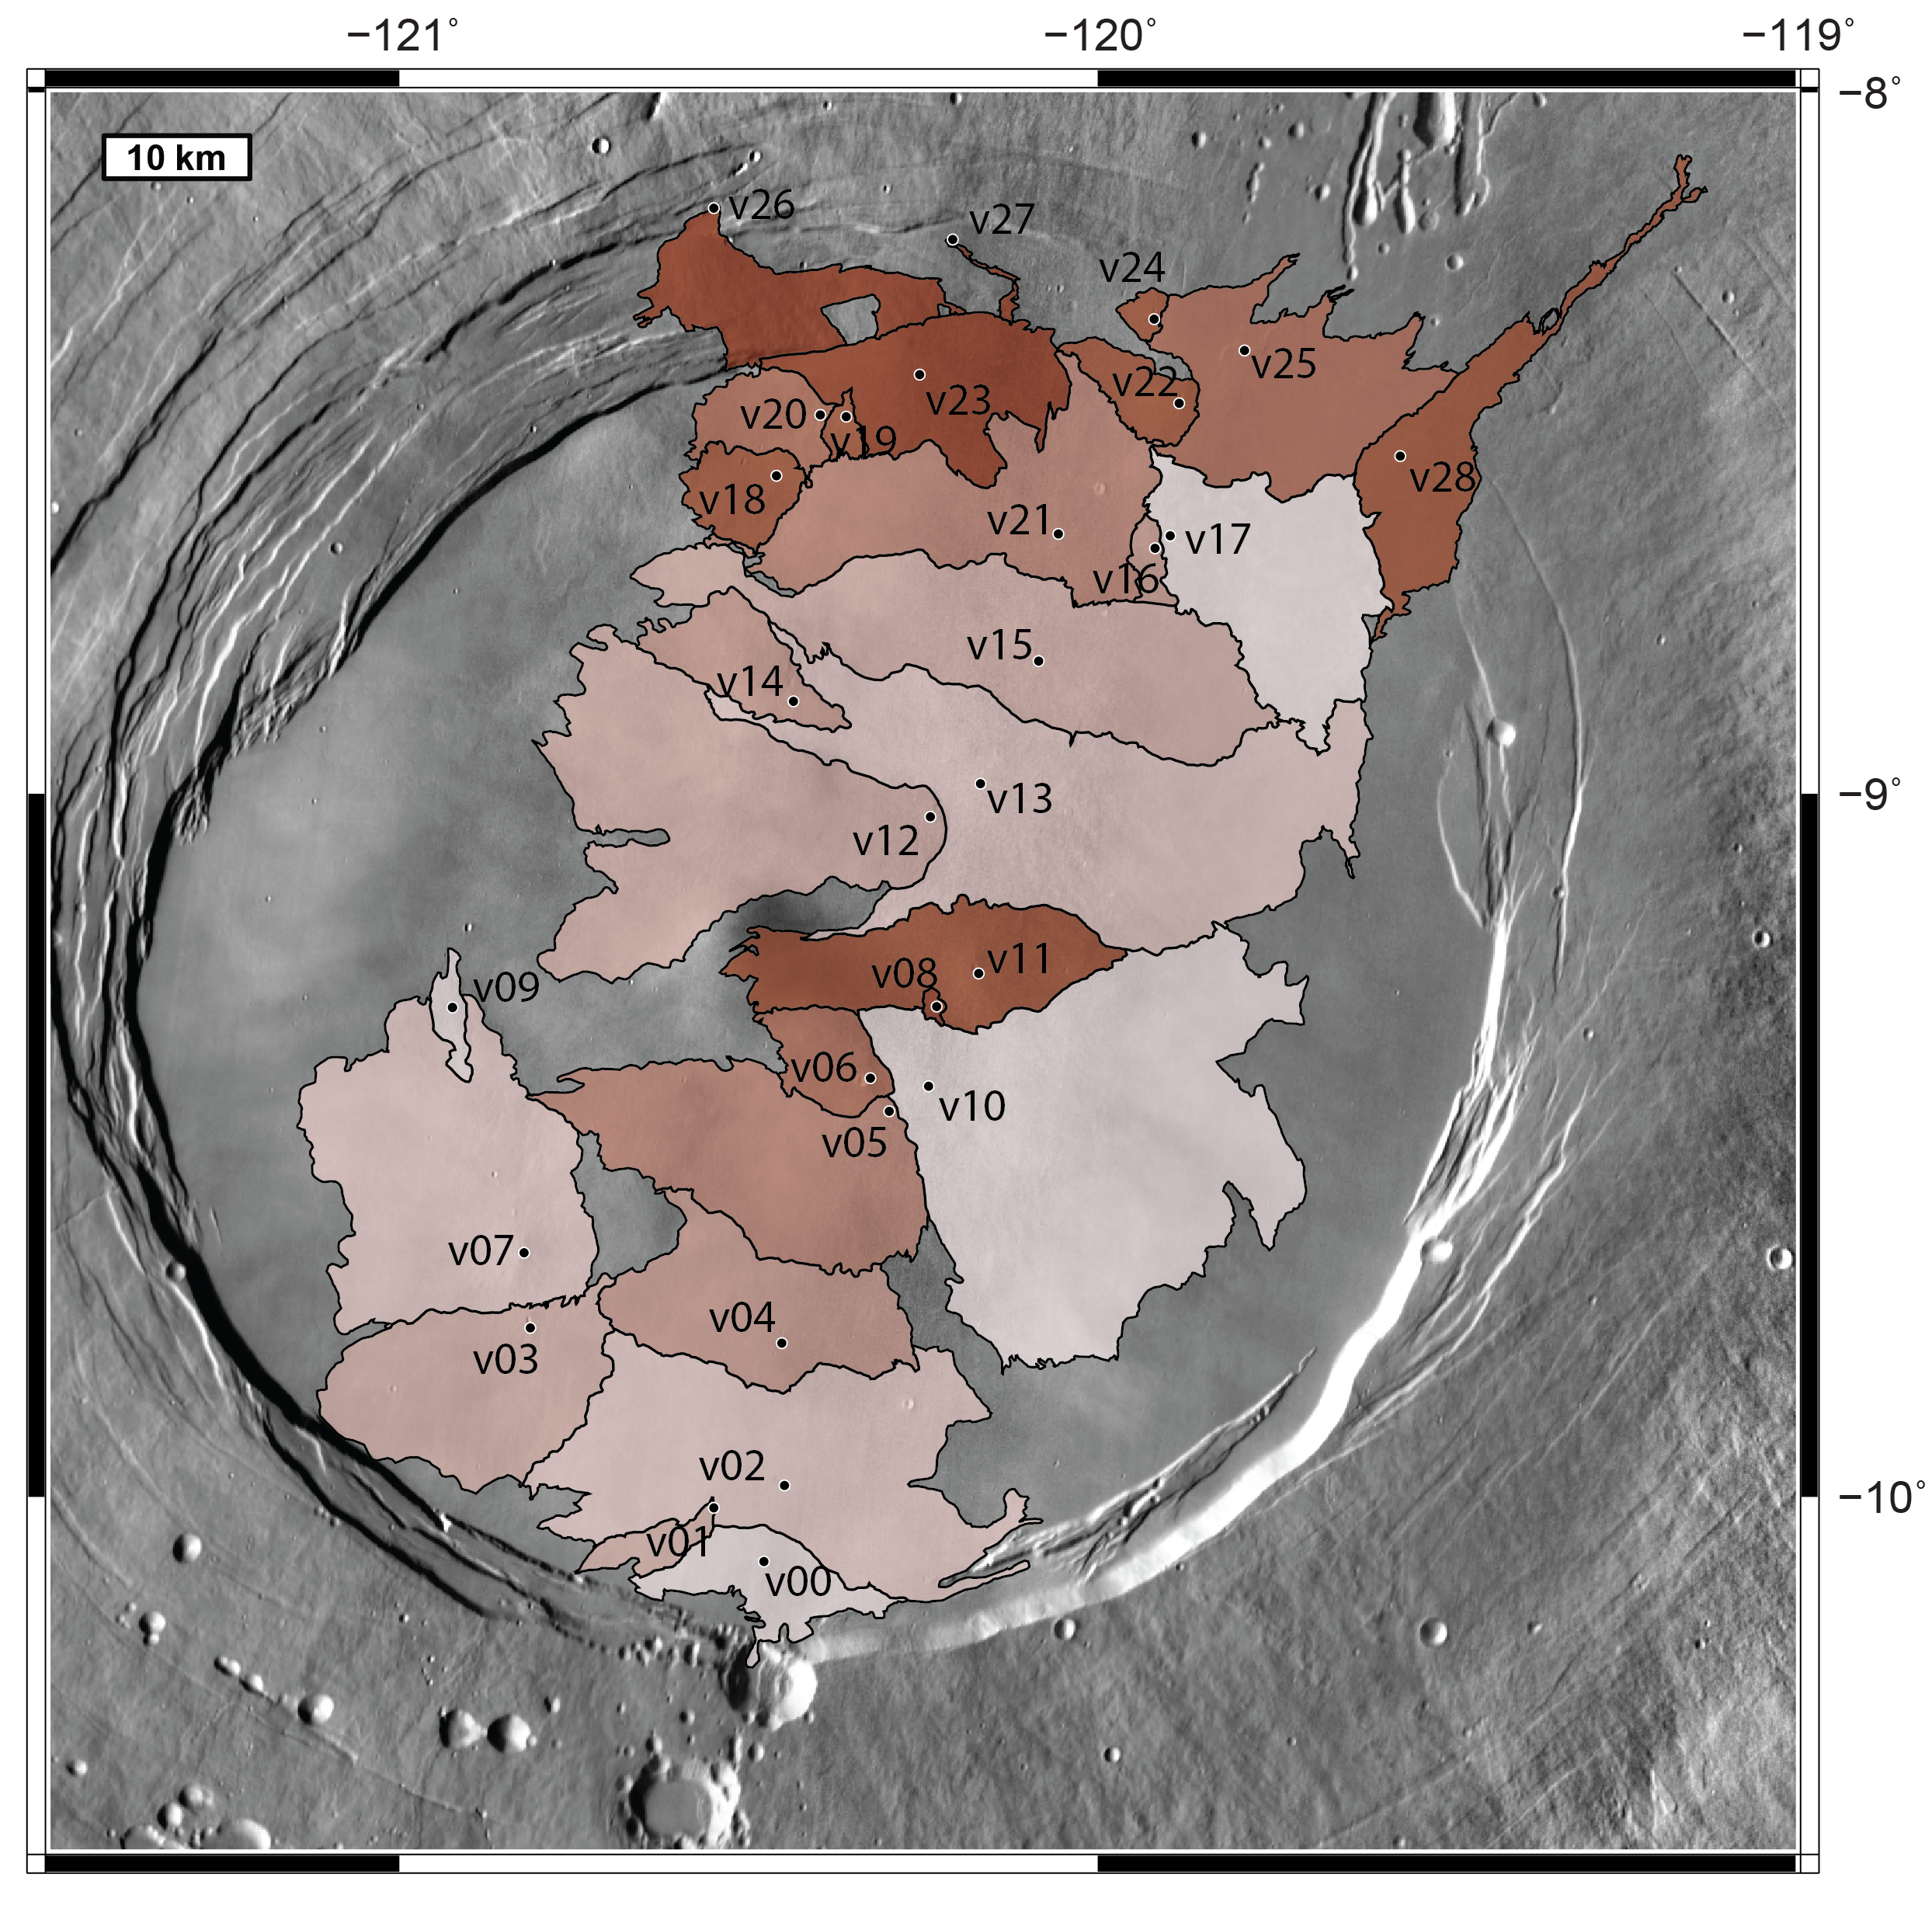
\includegraphics[width=1\textwidth]{figures/defense/arsia_mapstrat_300dpi.png}
	\end{columns}
	}
	
	%Segue to VERRM
	\frame{\frametitle{Ages: Information Conflicts}
	\begin{columns}
	\column{0.5\textwidth}
	%Examples: V00, V02, V04
		\begin{block}{Mean crater ages can agree stratigraphy...}
		\centering
		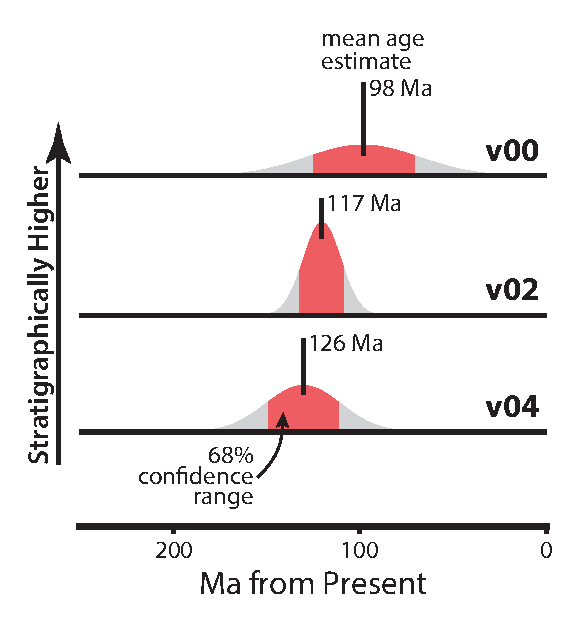
\includegraphics[width=0.8\textwidth]{figures/defense/crater_pdfs-000204.eps}
		\end{block}
	\column{0.5\textwidth}
		\centering
		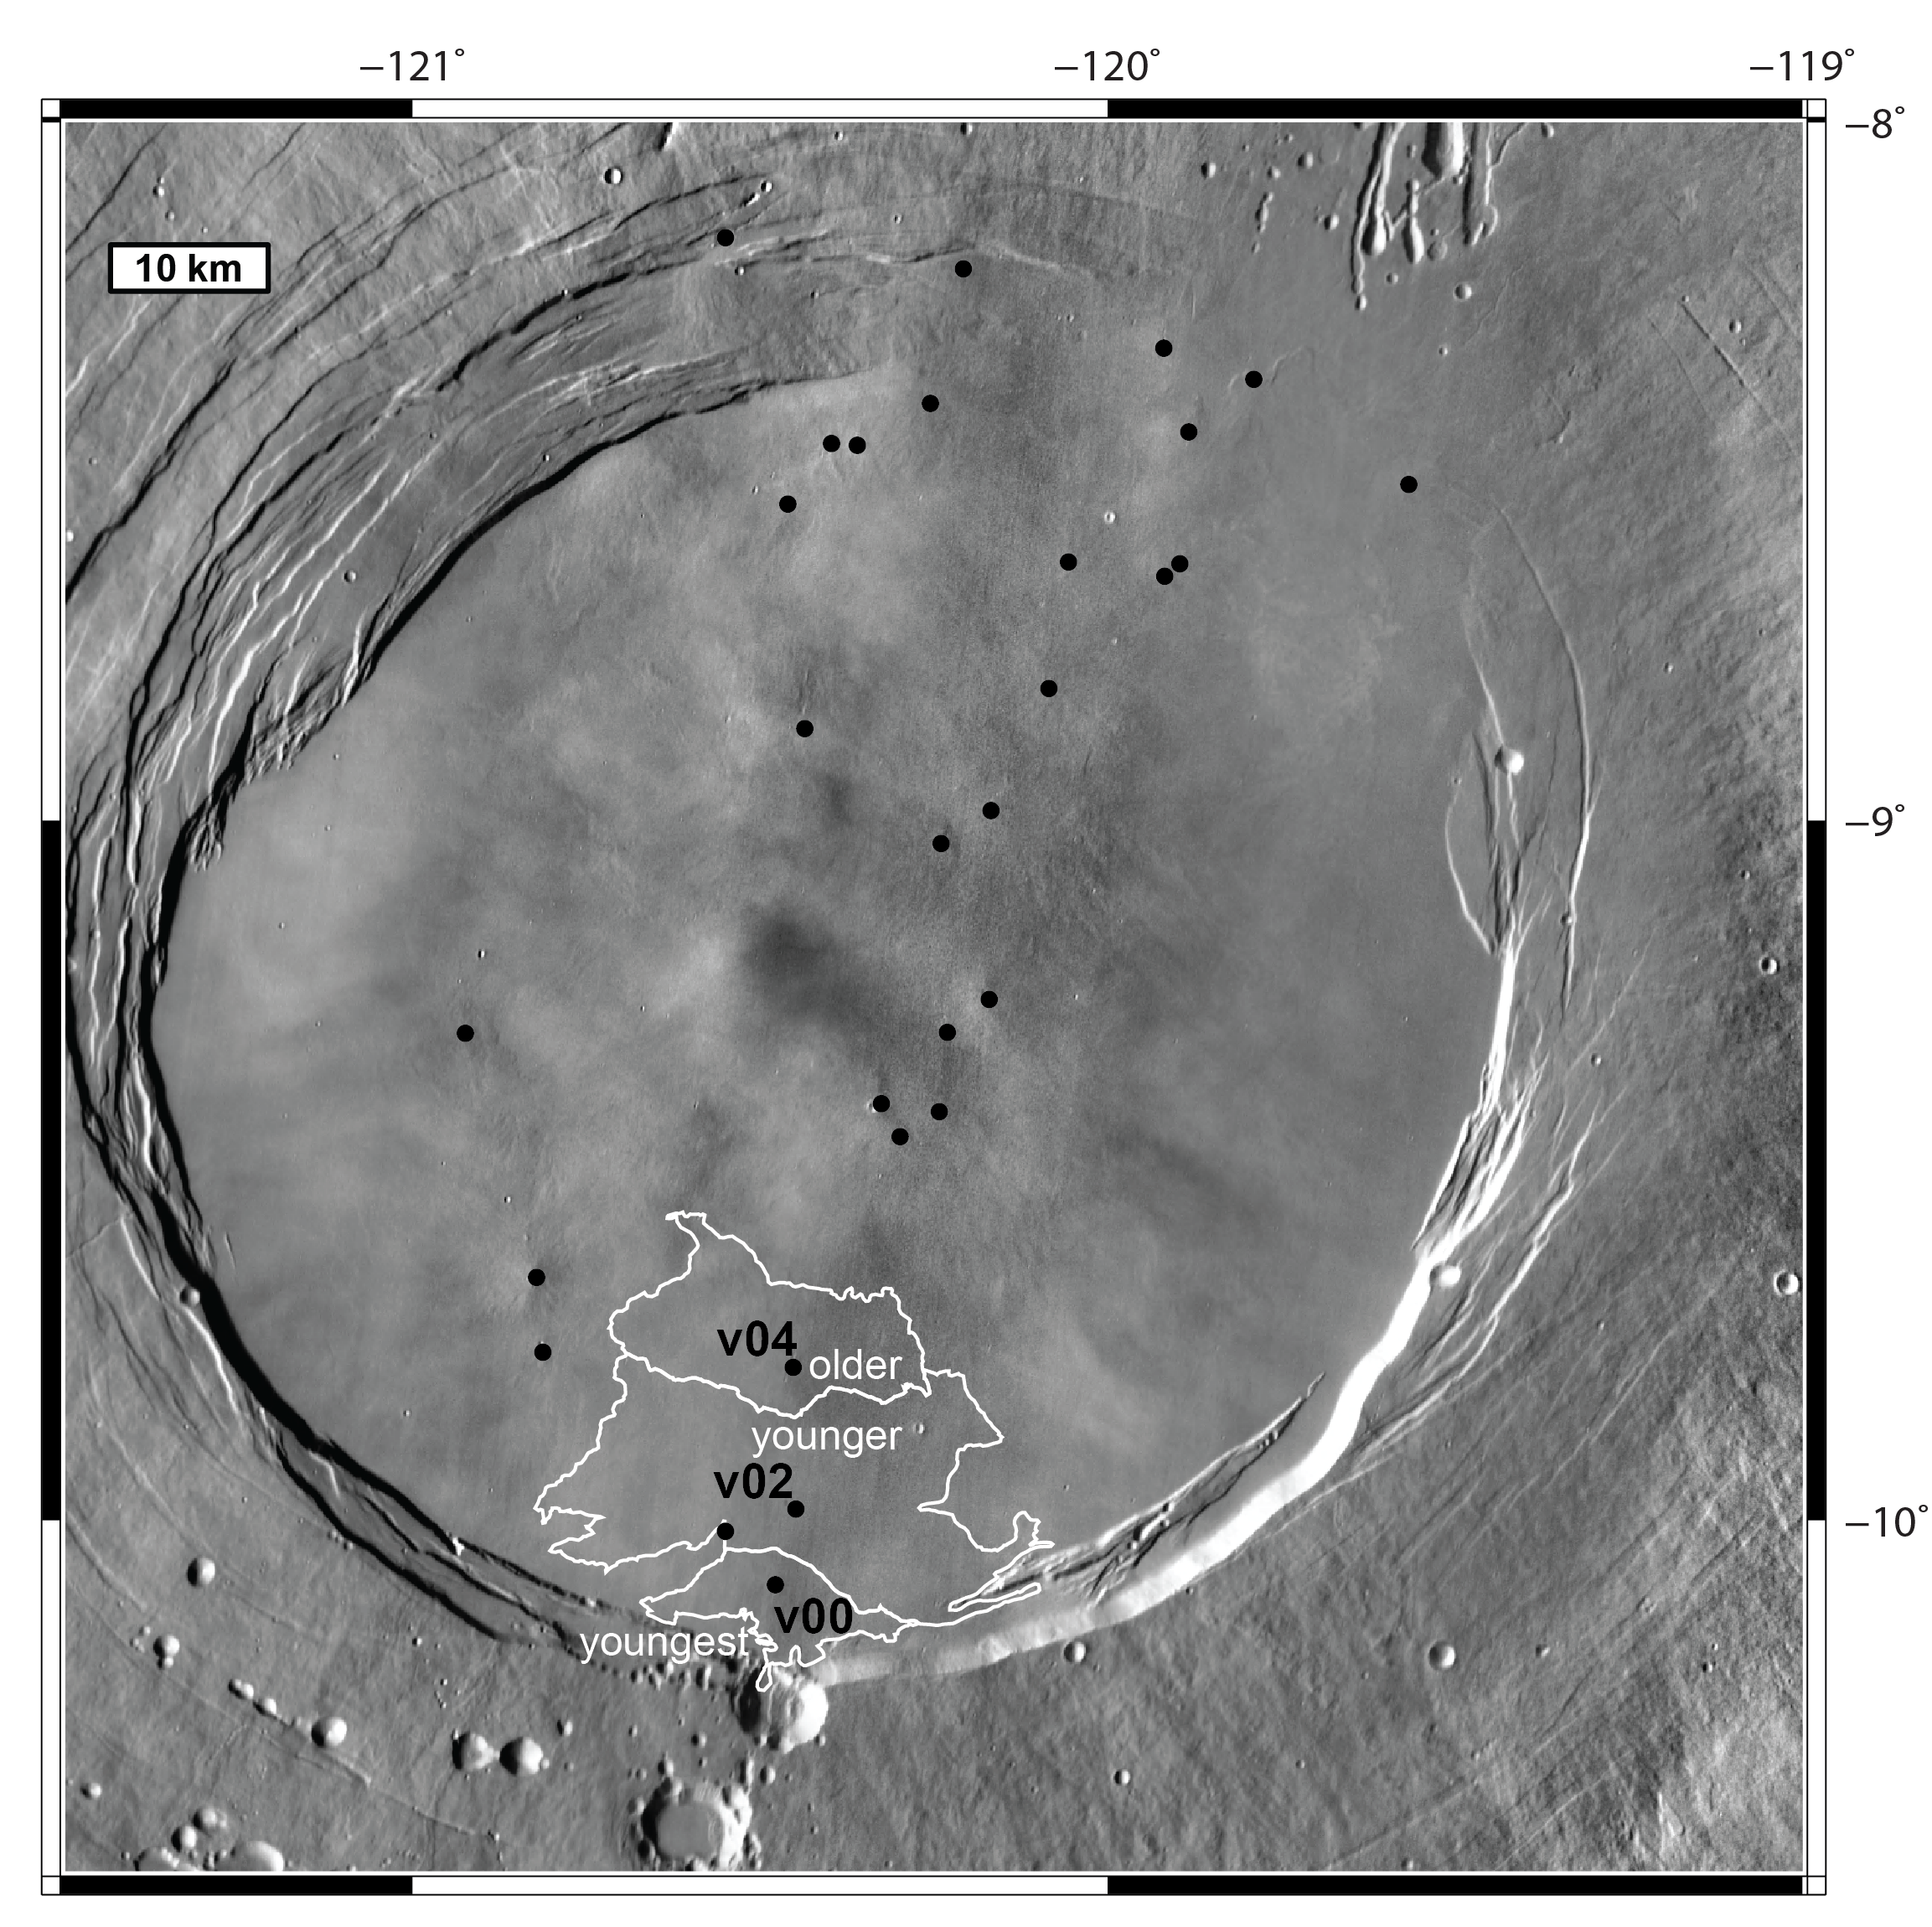
\includegraphics[width=1\textwidth]{figures/defense/arsia_0-2-4_300dpi.png}
	\end{columns}
	}

	\frame{\frametitle{Ages: Information Conflicts}
	\begin{columns}
	\column{0.5\textwidth}
	%          V25, V17
		\begin{block}{...or mean age can disagree with strat.}
		\centering
		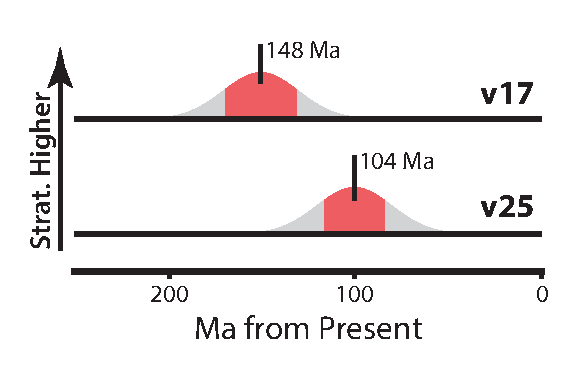
\includegraphics[width=0.8\textwidth]{figures/defense/crater_pdfs-2517.eps}
		
		\textbf{But by probabilistically modeling age, possible ages can still be identified}
		\end{block}
	\column{0.5\textwidth}
		\centering
		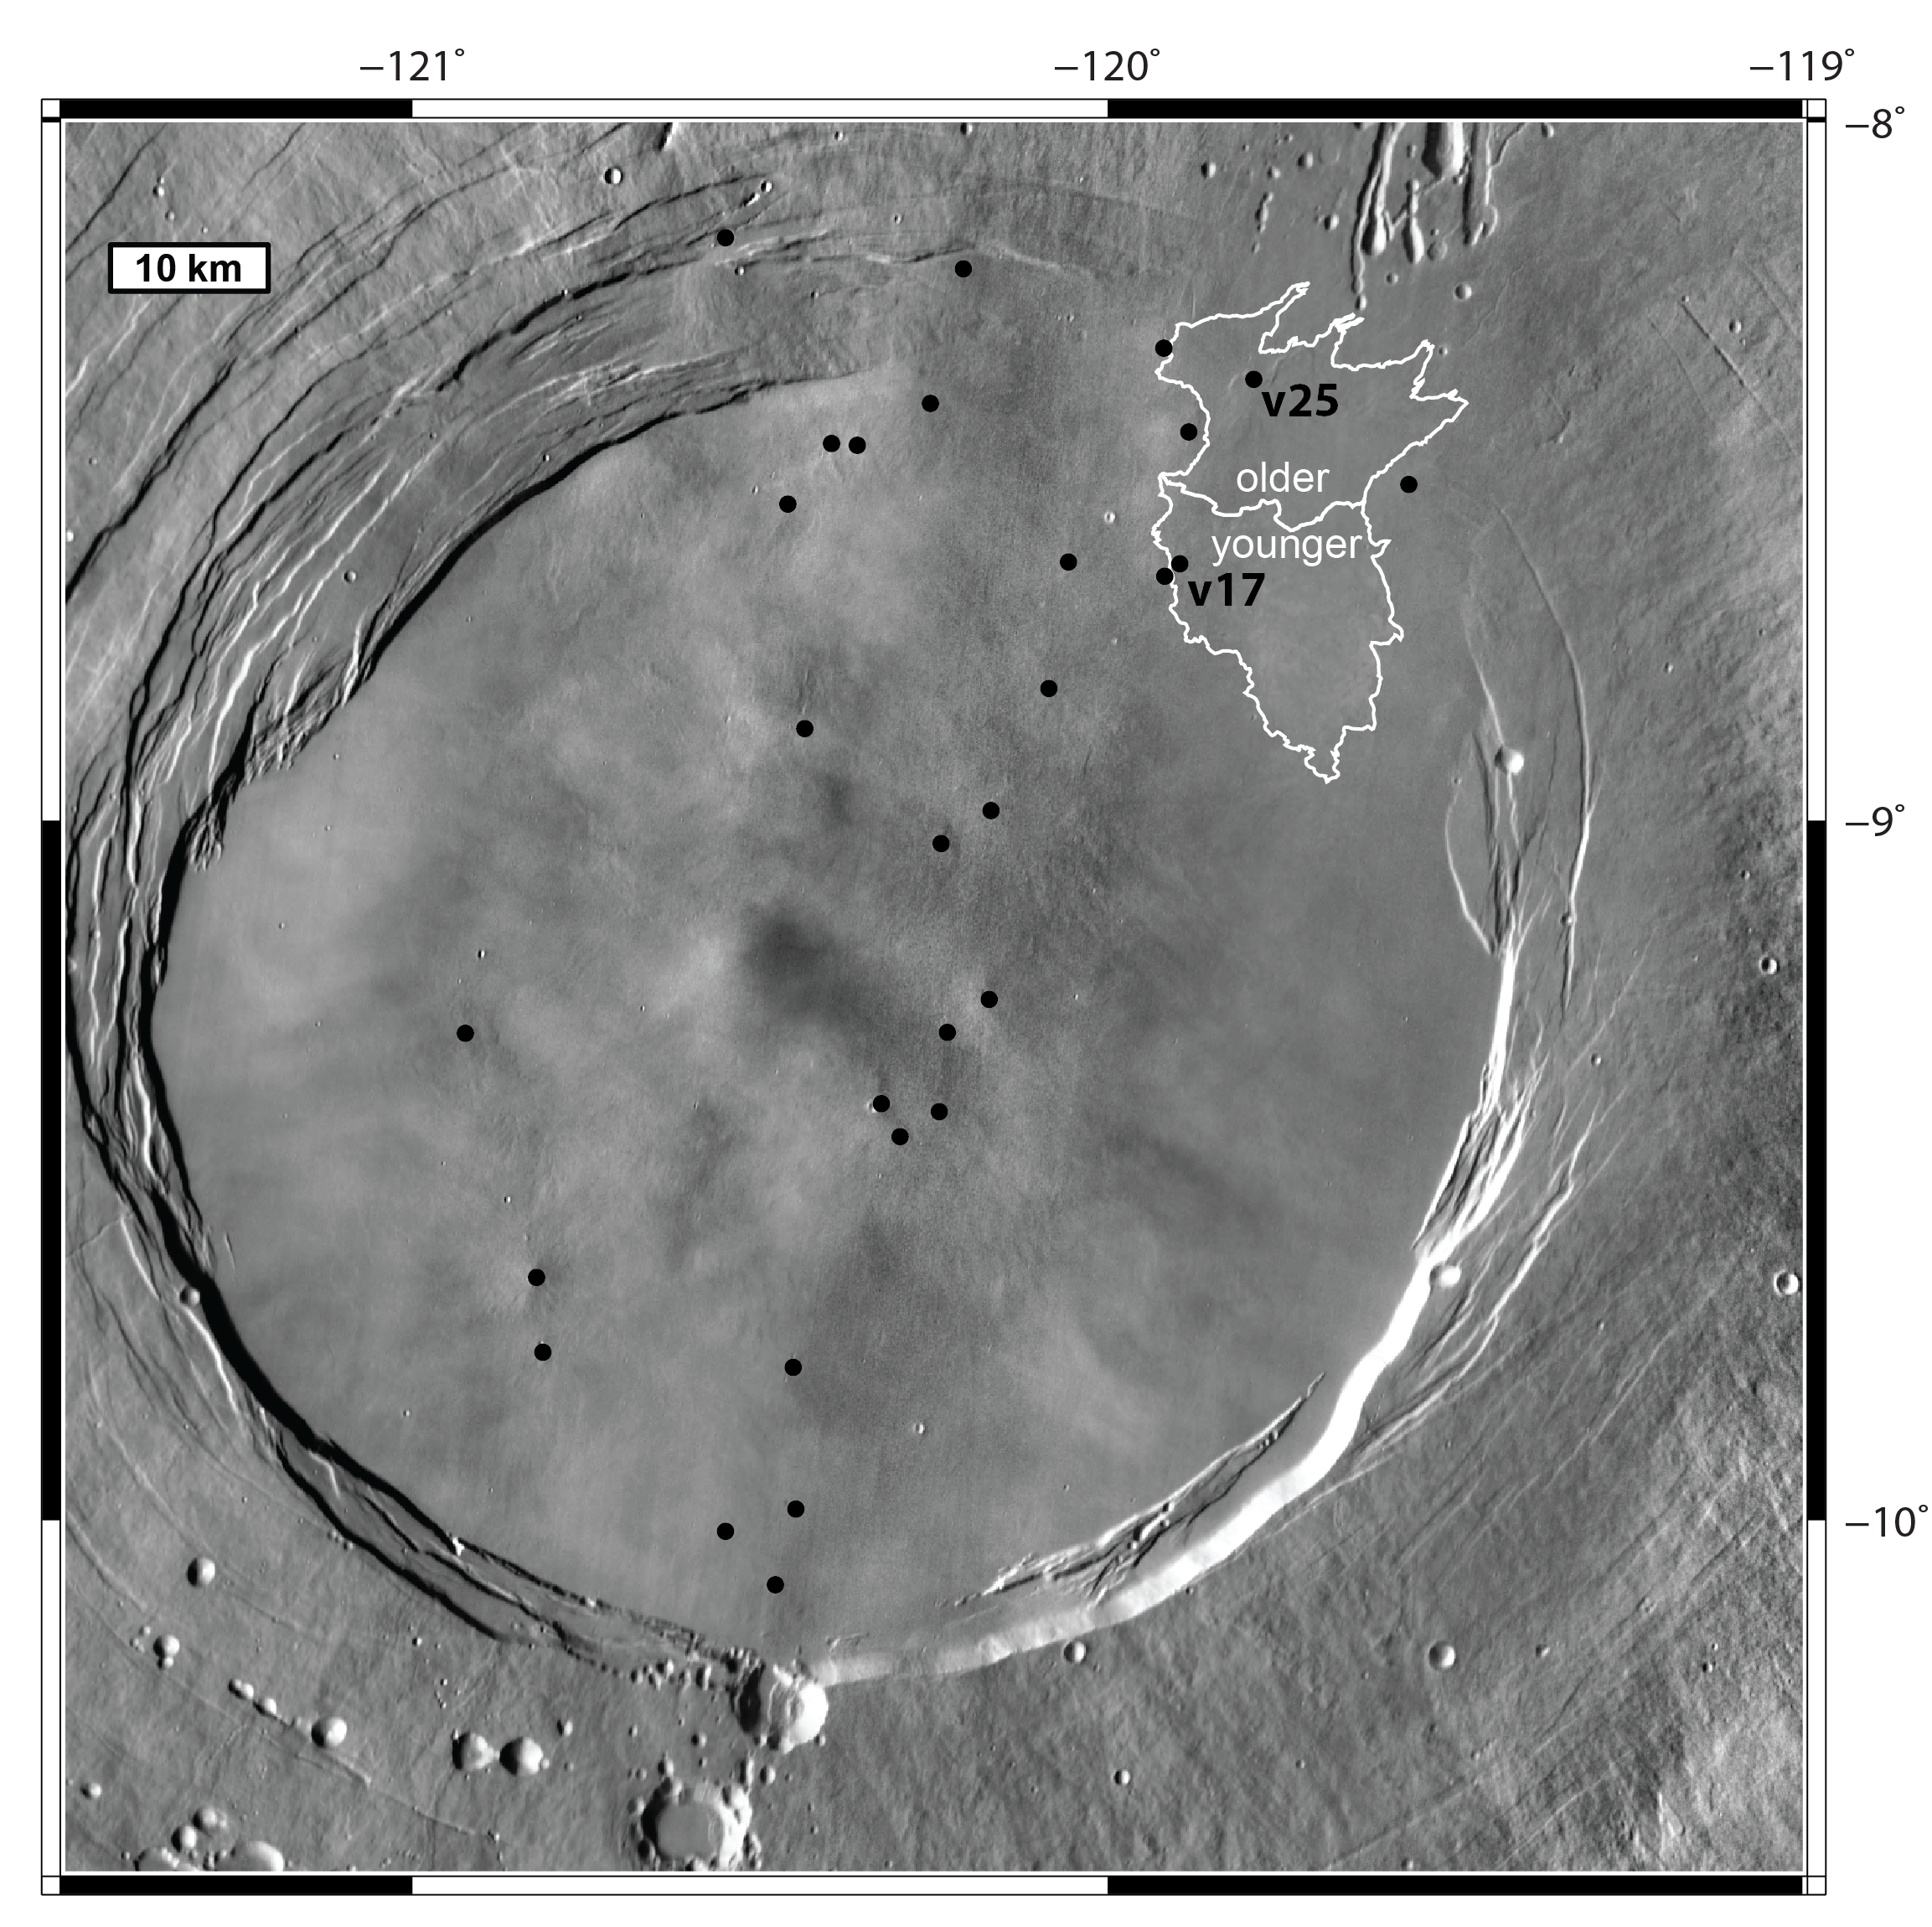
\includegraphics[width=1\textwidth]{figures/defense/arsia_17-25_300dpi.png}
	\end{columns}
	}

	\frame{\frametitle{Volcanic Event Recurrence Rate Model (VERRM)}
	%LPSC sketch
	\begin{block}{\textbf{Step 1:} Find potential ages of all events in the field (Monte Carlo)}
		\centering
		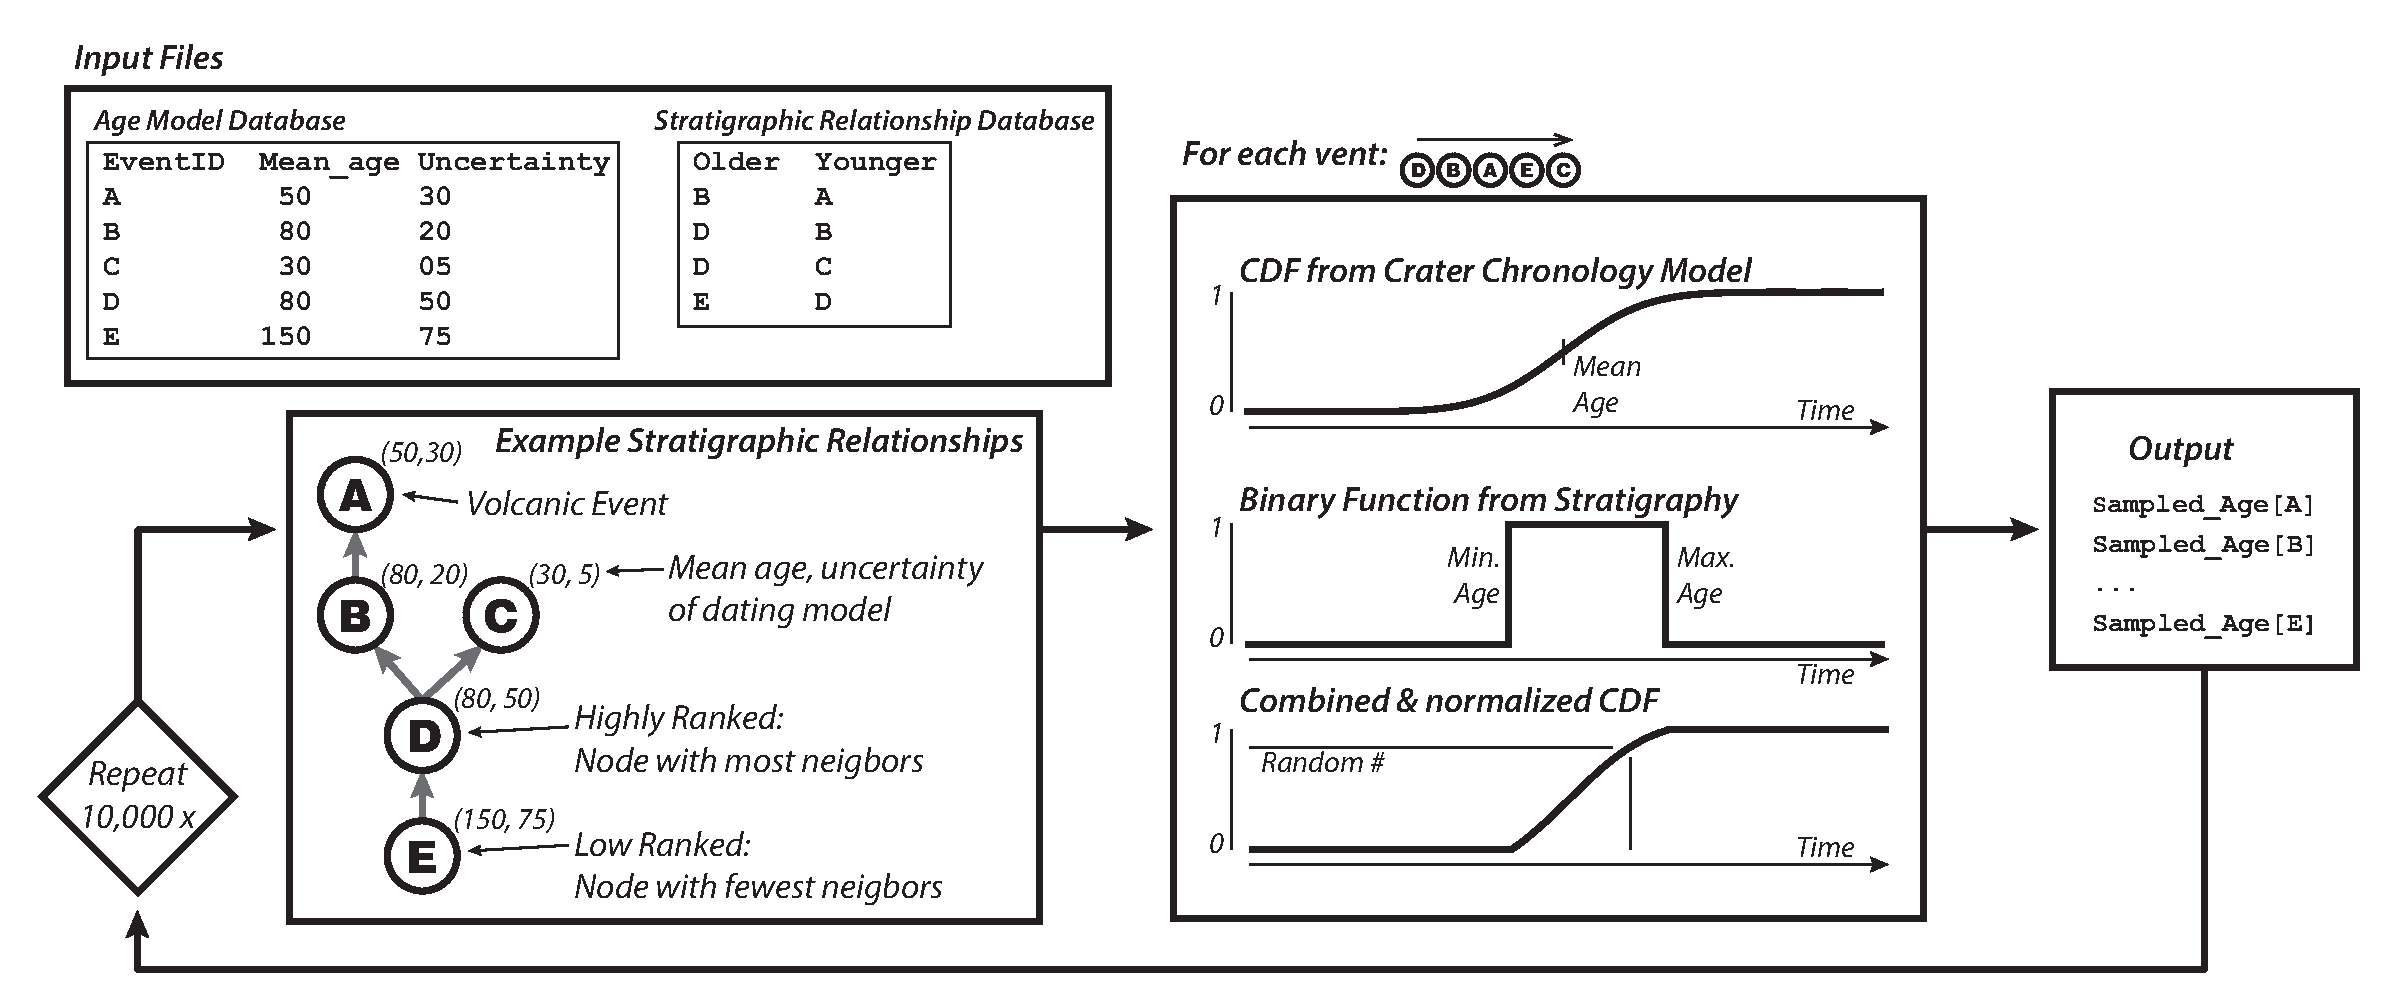
\includegraphics[width=1\textwidth]{figures/defense/verrm_flowchart.eps}
	\end{block}
	}
	
	\frame{\frametitle{Volcanic Event Recurrence Rate Model (VERRM)}
		\centering
		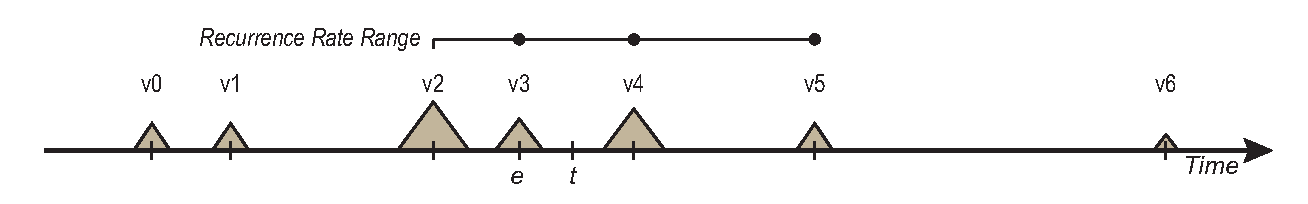
\includegraphics[width=0.9\textwidth]{figures/defense/RR_timeline.eps}
		\begin{block}{\textbf{Step 2:} Calculate Recurrence Rate of Volcanism}
			For each Monte Carlo simulation (i.e. each set of potential ages), model Recurrence Rate (RR) through time:\\[-1em]
			\begin{equation*}
			\text{RR}(t) = \frac{3}{\text{T}_{e-1} - \text{T}_{e+2}}
			\end{equation*}
		\end{block}\\[-1em]
		\begin{block}{\textbf{Step 3:} Calculate Magma Delivery Rate}
			Model Magma Delivery Rate (Flux) through time:\\[-0.5em]
			\begin{equation*}
			\text{Flux}(t) = \frac{\text{Volume}_e}{\text{T}_e-\text{T}_{e+1}}
			\end{equation*}
		\end{block}
	}

\subsection{Results}
	\frame{\frametitle{Results}
	\begin{block}{Recurrence Rate through time}
	\begin{columns}
	\column{0.55\textwidth}
	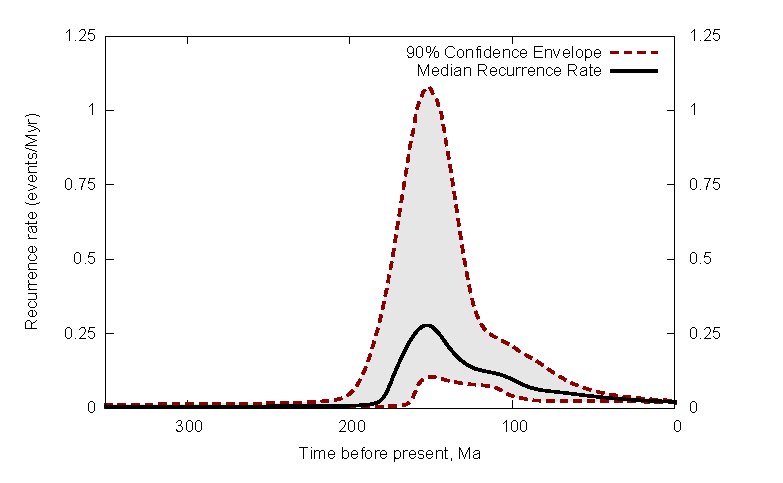
\includegraphics[width=1.1\textwidth]{figures/defense/VERRM_RR.eps}
	\column{0.45\textwidth}
		\begin{itemize}
			\item All 10,000 Recurrence Rate functions are combined
			\item Rate peaks at 150~Ma, producing 1 vent per 1-10~Myr (Median value: 0.25~events~Myr$^{-1}$)
			\item Rate has decreased monotonically: RR$(t=0)\rightarrow0$
		\end{itemize}
	\end{columns}
	\end{block}
	}

	\frame{\frametitle{Volume Flux}
	\begin{block}{Magma Delivery Rate through time}
	\begin{columns}
	\column{0.45\textwidth}
		\begin{itemize}
			\item All 10,000 Magma Delivery Rate functions are combined
			\item Median rate plateaus at at 150~Ma (0.4-3 km$^3$~Myr$^{-1}$), remains steady until 100~Ma before rapidly waning.
			\item Uncertainty in magma delivery rate is about 1~order of magnitude to either side of the median
		\end{itemize}
	\column{0.55\textwidth}
	\centering
	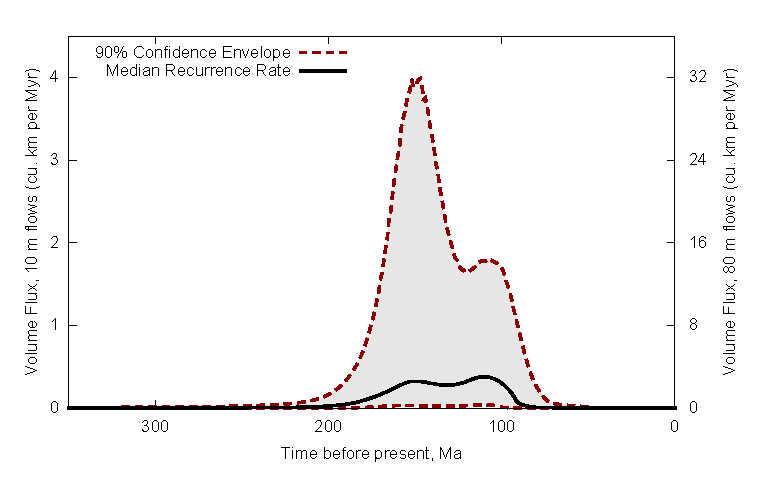
\includegraphics[width=1\textwidth]{figures/defense/VERRM_VF_THICK.eps}
	\end{columns}
	\end{block}
	}

\subsection{Implications}
	\frame{\frametitle{Tie-in with ashes and glaciers}
	\begin{columns}
	\column{0.5\textwidth}
		\begin{tikzpicture}
			\node (img1) {\includegraphics[width=1\textwidth]{figures/defense/arsia_overview.jpg}};
			%\pause
			\node (img2) at (img1.center) [xshift=2cm] {\includegraphics[height=0.98\textheight]{figures/defense/shean_graben.png}};
			\draw[red,thick] (-1.75,0.72) rectangle (-1.35,1.3);
		\end{tikzpicture}
	\column{0.5\textwidth}
		\begin{itemize}
			\item Extant glaciers are preserved on Western flank of Arsia
			\item Preserved for $\sim$200~Ma by ashes {\scriptsize(Kadish et al., \textit{P\&SS}, 2014)}
			\item If ashes were sourced near-summit {\scriptsize(Mouginis-Mark, \textit{GRL}, 2002)}, our effusive volcanism might be predated by explosive activity
		\end{itemize}
		
		\mbox{$\leftarrow$\scriptsize \textit{from Shean et al., JGR Planets, 2007}}
	\end{columns}
		
	}

	\frame{\frametitle{Model of waning volcanism of Arsia}
	\begin{columns}
	\column{0.45\textwidth}
	\begin{tikzpicture}
			\node (img1) {\includegraphics[width=1\textwidth]{figures/defense/VERRM_RR.eps}};
			%\pause
			\node at (-0.9,-0.78) [rotate=35] {\tiny waxing(?)};
			\node at (1.3,-0.6) [rotate=-23] {\tiny waning};
			\draw[red,thick,->] (-1.3,-1.25) -- (-0.2,-0.5);
			\draw[red,thick,->] (0.7,-0.5) -- (2,-1);
		\end{tikzpicture}
		\centering
		\includegraphics[width=0.6\textwidth]{figures/defense/arsia_overview.jpg}
	
	\column{0.55\textwidth}
	\begin{enumerate}
		\item Large magma chamber fed edifice-building, sometimes explosive eruptions {\scriptsize(Wilson et al., \textit{JGR}, 2001)}
		\item Ashes coated ice-rich deposits before 200~Ma
		\item The chamber cooled from waning magma flux
		\item Volcanism evolved from explosive to effusive as magma waned
		\item Volcanism is now in haitus (RR$(t=0)\rightarrow0$)
	\end{enumerate}
	\end{columns}
	}

\section{Conclusions}
	\frame{\frametitle{Conclusions}
	\begin{block}{Arsia Mons}
	\begin{enumerate}
			\item Late volcanism at Arsia Mons emplaced a volcanic field in its caldera
			\item Multiple dating methods used on lavas can be combined to estimate rate of volcanism, which peaked 150~million years ago
			\item Volcanism waned and likely ceased 10-90~million years ago
			\item This field might be related to a larger waning of volcanism at Arsia
			\item Vents in this field are less concentrated than vents in terrestrial volcanic fields
			\item Lava flows are an order of magnitude larger in volume than flows in most terrestrial fields
		\end{enumerate}
	\end{block}
	}

	\frame{\frametitle{Conclusions}
	\begin{block}{Overall Conclusions}
	\begin{itemize}
			\item Volcanic fields have complex, voluminous roots
			\item Emplacement of lavas in these fields can be modeled
			\item Volcanic vent distribution in fields has a wide variation across the solar system
			\item These tools can be used to gain knowledge about volcanic fields on Mars with spaceborne instruments
		\end{itemize}
	\end{block}
	\centering
	\includegraphics[width=0.25\textwidth]{figures/defense/CedarMtn-photo.png}
	\includegraphics[width=0.3\textwidth]{figures/defense/pulse_examples_300dpi.png}
	\includegraphics[width=0.2\textwidth,clip,trim=0cm 0cm 3.2cm 0cm ]{figures/chapter-spatial_density/arsia_kde_300dpi.png}
	\includegraphics[width=0.22\textwidth]{figures/defense/arsia_mapstrat_300dpi.png}
	}


\section{}
	\frame{\frametitle{Acknowledgements}
	%Pictures: Rocco/Judy with a snowman
	%Solfaterra picnic OROROROR 3981 - solfatera!!
	%Chuck 4091 - pompei %or 3743 columnar basalts
	\begin{block}{The Intrepid Committee!}
	Chuck Connor, Jake Bleacher, Rocco Malservisi, Matt Pasek, and Tim Dixon
	\begin{tikzpicture}
		\node (img5) at (3,0) {\includegraphics[height=2.5cm]{figures/defense/vanity/vCrewMissionTraining.jpg}};
		\node (img3) at (5.75,0) {\includegraphics[height=2.5cm]{figures/defense/vanity/rocco.jpg}};
		\node (img4) at (8.4,0) {\includegraphics[height=2.5cm]{figures/defense/vanity/matt_pasek_500.jpg}};
		\node (img2) at (0,0) {\includegraphics[height=2.5cm]{figures/defense/vanity/chuck.jpg}};
		\node (img1) at (10.7,0) {\includegraphics[height=2.5cm]{figures/defense/vanity/tim.jpg}};		
	\end{tikzpicture}
	\end{block}
	}

	\frame{\frametitle{Questions?}
	\centering
	\includegraphics[width=0.8\textwidth]{figures/defense/vanity/lava_thing.jpg}
	}


\end{document}
